\documentclass[10pt,a4paper,oneside]{article}

% ---------------------------------------------------------------------------
% features-energia-en.tex -- en-US version of `features-energia.tex`.
%
% PARITY WITH THE PORTUGUESE FILE. This is a translation, not a fork: both
% documents carry the same sections, the same 66 features, the same numbers
% and the same references. A change in one belongs in the other. The catalog
% lives in `features/catalogo.csv` (pt) and `features/catalogo-en.csv` (en);
% `features/gerar.py` checks that the two agree on ids, levels, clients,
% phases, map fit and dependencies before it generates the tables.
%
% DELIBERATE DIVERGENCES FROM THE SOURCE FILE:
%
%   `babel` loads `american`. The cover block, the footer and the NOTE box
%   come from the shared preamble with Portuguese labels; they are redefined
%   below, locally, so the preamble keeps serving the Portuguese documents
%   unchanged.
%
%   Numbers follow en-US: decimal point, comma as thousands separator.
%
%   The phase tag `fora` is `out`. Feature ids, module codes, agency names,
%   dataset names and regulation numbers stay as in the source: they are
%   identifiers.
%
% Base preamble of the repository: font, type area, packages, caption, title
% and header. Compile from inside `docs/product/`.
% ---------------------------------------------------------------------------
\usepackage[american]{babel}
% =====================================================================
%  Preâmbulo base: pacotes, tipografia e convenções de todo documento
%  LaTeX do repositório
%
%  Origem: `config/preambulo.tex` do documento de projeto do rhae-sensor.
%  As seções abaixo seguem a ordem de lá, e o que difere está marcado
%  com DIFERENÇA.
%
%  Convenções tipográficas e de apresentação adotadas
%    ISO 216        formato A4
%    ISO 80000-1    números e unidades (vírgula decimal, espaço fino entre
%                   grupos de três algarismos, unidade em tipo romano)
%    Tabelas sem filetes verticais (booktabs); legenda de tabela acima,
%    de figura abaixo.
%
%  Uso, antes do `\begin{document}`:
%    report/*.tex          via `\usepackage{estilo-reporte}`, que carrega este
%    docs/product/*.tex    % =====================================================================
%  Preâmbulo base: pacotes, tipografia e convenções de todo documento
%  LaTeX do repositório
%
%  Origem: `config/preambulo.tex` do documento de projeto do rhae-sensor.
%  As seções abaixo seguem a ordem de lá, e o que difere está marcado
%  com DIFERENÇA.
%
%  Convenções tipográficas e de apresentação adotadas
%    ISO 216        formato A4
%    ISO 80000-1    números e unidades (vírgula decimal, espaço fino entre
%                   grupos de três algarismos, unidade em tipo romano)
%    Tabelas sem filetes verticais (booktabs); legenda de tabela acima,
%    de figura abaixo.
%
%  Uso, antes do `\begin{document}`:
%    report/*.tex          via `\usepackage{estilo-reporte}`, que carrega este
%    docs/product/*.tex    % =====================================================================
%  Preâmbulo base: pacotes, tipografia e convenções de todo documento
%  LaTeX do repositório
%
%  Origem: `config/preambulo.tex` do documento de projeto do rhae-sensor.
%  As seções abaixo seguem a ordem de lá, e o que difere está marcado
%  com DIFERENÇA.
%
%  Convenções tipográficas e de apresentação adotadas
%    ISO 216        formato A4
%    ISO 80000-1    números e unidades (vírgula decimal, espaço fino entre
%                   grupos de três algarismos, unidade em tipo romano)
%    Tabelas sem filetes verticais (booktabs); legenda de tabela acima,
%    de figura abaixo.
%
%  Uso, antes do `\begin{document}`:
%    report/*.tex          via `\usepackage{estilo-reporte}`, que carrega este
%    docs/product/*.tex    \input{../../report/config/preambulo}
%
%  FORMA DE MANUAL TÉCNICO. Fonte, números, legendas e pacotes vêm da
%  origem. A forma da página não: é de manual de referência, e não de
%  artigo. Coluna única, títulos recuados para a esquerda do texto,
%  rodapé com identificação e "página X de Y" em toda página, avisos com
%  palavra de sinal (ANSI Z535.6), passos numerados e histórico de
%  revisões (IEC/IEEE 82079-1). O desenho de página segue a classe
%  `refman` do CTAN.
%
%  O documento carrega `babel` ANTES deste arquivo. Documento deitado, que
%  existe para caber tabela larga, carrega também `geometry` antes; aí a
%  margem de manual não entra e os títulos não avançam.
%
%  Motor: pdflatex. Charis SIL, newtxmath e Bera Mono entram como Type 1
%  em T1, e a matemática do newtxmath não passa pelo `unicode-math`.
% =====================================================================
\RequirePackage{iftex}
\RequirePDFTeX
% Este arquivo entra tanto de um `.tex` quanto de dentro do
% `estilo-reporte.sty`, onde o `@` ja e letra. O codigo de categoria e
% devolvido como estava, e nao forcado a "outro" no fim.
\edef\pbrestauraarroba{\catcode`\noexpand\@=\the\catcode`\@\relax}
\makeatletter

% ---------------------------------------------------------------------
%  Fontes, idioma e microtipografia
% ---------------------------------------------------------------------
\usepackage[T1]{fontenc}
\usepackage[utf8]{inputenc}
% DIFERENÇA: o idioma é do documento, porque há documento em inglês.
\@ifpackageloaded{babel}{}{\usepackage[brazilian]{babel}}
\usepackage{CharisSIL}
\usepackage[charter]{newtxmath}
\usepackage[scaled=0.83]{beramono}
\usepackage[protrusion=true,expansion=true,tracking=true]{microtype}
\SetTracking{encoding=*,shape=sc}{40}
% DIFERENÇA: a origem não usa sem serifa. Os documentos daqui pedem
% `\sffamily` em título, tabela e nota; sem esta linha ela cairia na
% Computer Modern Sans, que não pertence ao conjunto. Uma família só.
\renewcommand{\sfdefault}{\rmdefault}

% DIFERENÇA: mancha de manual, e não a coluna de 468 pt da origem. A4 com
% 22 mm de margem de cada lado, 166 mm úteis. O texto corre em 152 mm e
% os 14 mm da esquerda são o recuo dos títulos: o bastante para o título
% sair do alinhamento do texto, sem deixar coluna vazia ao lado dele. A
% primeira versão reservava 40 mm, e a margem ficava em branco em toda
% página que não fosse título; o documento crescia um terço só por isso.
% `\margemmanual` é quanto os títulos, o cabeçalho e o rodapé avançam
% para a esquerda; vale zero quando o documento traz mancha própria.
% A altura é de 253 mm, a mesma da mancha anterior, porque as tabelas
% deitadas foram dimensionadas para ela.
\newlength{\margemmanual}
\@ifpackageloaded{geometry}{\setlength{\margemmanual}{0pt}}{%
  \setlength{\margemmanual}{14mm}%
  \usepackage[a4paper,left=36mm,right=22mm,top=20mm,bottom=24mm,
              headheight=14pt,headsep=7mm,footskip=12mm]{geometry}}

\usepackage{amsmath}
\usepackage[dvipsnames,table]{xcolor}
\usepackage{graphicx}
\usepackage{tikz}
\usepackage{booktabs}
\usepackage{tabularx}
\usepackage{array}
\usepackage{xltabular}
\usepackage{float}
\usepackage{pdflscape}
\usepackage{rotating}
% Página com o conteúdo girado, mas exibida em retrato no leitor de PDF
\newenvironment{paisagemretrato}{\begingroup\def\PLS@AddRotate##1{}\landscape}{\endlandscape\endgroup}
\usepackage{enumitem}
\usepackage{changepage}
\usepackage[most]{tcolorbox}
\usepackage{caption}
\usepackage{titlesec}
\usepackage{fancyhdr}
\usepackage{lastpage}
\usepackage{csquotes}
\usepackage{siunitx}
% DIFERENÇA: sem `biblatex`. Nenhum documento daqui tem `.bib`; as
% referências são listas escritas à mão.
\usepackage{xurl}
\usepackage[hidelinks,pdfusetitle]{hyperref}

% ---------------------------------------------------------------------
%  Números e unidades (ISO 80000-1)
% ---------------------------------------------------------------------
\sisetup{
  output-decimal-marker = {,},
  group-separator       = {\,},
  group-minimum-digits  = 4,
  exponent-product      = \cdot,
  uncertainty-mode      = separate,
  range-phrase          = {\,a\,},
  list-pair-separator   = {\ e\ },
  list-final-separator  = {\ e\ },
  per-mode              = symbol,
}

% ---------------------------------------------------------------------
%  Parágrafo, listas e flutuantes
% ---------------------------------------------------------------------
% DIFERENÇA: parágrafo em bloco, separado por espaço e sem recuo, que é
% o de manual; a origem recua 1 em.
\setlength{\parindent}{0pt}
\setlength{\parskip}{0.45em plus 0.1em}
\linespread{1.04}
\setlist{itemsep=0.1em,topsep=0.3em,leftmargin=1.4em}
\renewcommand{\arraystretch}{1.15}
\setlength{\tabcolsep}{5pt}
\setlength{\LTpre}{0.8em}
\setlength{\LTpost}{0.4em}

% Legendas no padrão Elsevier: \enquote{Fig. 1.} seguido do texto, alinhado à esquerda;
% \enquote{Tabela 1} numa linha e o título na linha seguinte
\DeclareCaptionLabelSeparator{travessao}{\ — }
% `babel` guarda os nomes por idioma, e o nome da opção varia entre os
% documentos. Entra em cada um que estiver carregado.
\@for\pb@idioma:=brazilian,brazil,portuguese,portuges,american,english\do{%
  \@ifundefined{captions\pb@idioma}{}{%
    \expandafter\addto\csname captions\pb@idioma\endcsname{\renewcommand{\figurename}{Fig.}}}}
\captionsetup{font=footnotesize,labelfont=bf,justification=justified,
              singlelinecheck=false,skip=5pt}
\captionsetup[figure]{position=bottom,labelsep=period}
\captionsetup[table]{position=top,labelsep=newline}
% DIFERENÇA: a origem fixa todo flutuante onde aparece (`H`). Aqui ele
% tenta o lugar e, se não couber no resto da página, sobe para a seguinte
% e o texto continua: com `H`, a tabela que não cabia deixava o fim da
% página em branco.
\floatplacement{table}{!htbp}
\floatplacement{figure}{!htbp}
\renewcommand{\topfraction}{0.9}
\renewcommand{\bottomfraction}{0.8}
\renewcommand{\textfraction}{0.08}
\renewcommand{\floatpagefraction}{0.75}

\newcolumntype{Y}{>{\raggedright\arraybackslash}X}
\newcolumntype{L}[1]{>{\raggedright\arraybackslash}p{#1}}
\newcolumntype{C}[1]{>{\centering\arraybackslash}p{#1}}
\newcolumntype{R}[1]{>{\raggedleft\arraybackslash}p{#1}}

% ---------------------------------------------------------------------
%  Títulos de seção (ISO 2145)
% ---------------------------------------------------------------------
% DIFERENÇA: título de manual. Seção e subseção avançam 14 mm para a
% esquerda do texto e ocupam a largura útil; a seção leva um fio acima.
% Número sem ponto final, três níveis numerados. Os três níveis têm o
% corpo do texto ou pouco mais: o nível se lê pelo fio, pelo recuo e
% pelo itálico do terceiro, e não pelo tamanho.
\setcounter{secnumdepth}{3}
\titleformat{\section}[block]
  {\titlerule[0.8pt]\vspace{0.5ex}\normalfont\large\bfseries\raggedright}{\thesection}{0.8em}{}
\titleformat{\subsection}{\normalfont\normalsize\bfseries\raggedright}{\thesubsection}{0.8em}{}
\titleformat{\subsubsection}{\normalfont\normalsize\bfseries\itshape\raggedright}{\thesubsubsection}{0.8em}{}
\titlespacing*{\section}{-\margemmanual}{1.5em plus 0.4em minus 0.2em}{0.5em plus 0.1em}
\titlespacing*{\subsection}{-\margemmanual}{1.1em plus 0.3em minus 0.2em}{0.3em plus 0.1em}
\titlespacing*{\subsubsection}{0pt}{0.9em plus 0.2em minus 0.2em}{0.2em}

% ---------------------------------------------------------------------
%  Identificação, cabeçalho e rodapé
% ---------------------------------------------------------------------
% Todo campo é do documento, por `\renewcommand` depois deste arquivo.
% Sem isso: o código é o nome do arquivo, a data é a da compilação em
% ISO 8601, e versão e responsável ficam vazios e somem.
\providecommand{\doctitulo}{}
\providecommand{\docsubtitulo}{}
\providecommand{\doccodigo}{\jobname}
\providecommand{\docversao}{}
\providecommand{\docresponsavel}{}
\providecommand{\docdata}{\the\year-\two@digits\month-\two@digits\day}

% Cabeçalho: título à esquerda, seção corrente à direita. Rodapé: código,
% versão e data à esquerda, "página X de Y" à direita. Os dois ocupam a
% largura útil, margem de título incluída.
\newcommand{\pb@identificacao}{%
  \texttt{\doccodigo}%
  \ifx\docversao\@empty\else\enspace\textperiodcentered\enspace versão \docversao\fi
  \enspace\textperiodcentered\enspace\docdata}
\pagestyle{fancy}
\fancyhf{}
\fancyhfoffset[L]{\margemmanual}
\fancyhead[L]{\footnotesize\bfseries\doctitulo}
\fancyhead[R]{\footnotesize\itshape\nouppercase{\rightmark}}
\fancyfoot[L]{\footnotesize\pb@identificacao}
\fancyfoot[R]{\footnotesize\thepage\ de \pageref*{LastPage}}
\renewcommand{\headrulewidth}{0.4pt}
\renewcommand{\footrulewidth}{0.4pt}
\fancypagestyle{plain}{}
% Página de rosto: sem cabeçalho, porque o título já está nela.
\fancypagestyle{rosto}{\fancyhead{}\renewcommand{\headrulewidth}{0pt}}

% ---------------------------------------------------------------------
%  Marca
% ---------------------------------------------------------------------
% DIFERENÇA: a origem não tem marca. Aqui todo documento abre com o
% logotipo Solara, versão para fundo claro. O caminho depende de onde se
% compila: `report/` ou `docs/product/`.
\IfFileExists{../docs/img/solara-logo-on-light.png}%
  {\newcommand{\marcaarquivo}{../docs/img/solara-logo-on-light.png}}%
  {\newcommand{\marcaarquivo}{../img/solara-logo-on-light.png}}
% \marcadoc[largura]: o logotipo tem proporção 7:1, então 30 mm dão
% 4,3 mm de altura.
\newcommand{\marcadoc}[1][30mm]{\includegraphics[width=#1]{\marcaarquivo}}

% ---------------------------------------------------------------------
%  Rosto e histórico de revisões
% ---------------------------------------------------------------------
% \rosto: marca, título, subtítulo e a tabela de identificação. Lê os
% campos `\doc...`; linha de campo vazio não sai.
\newcommand{\pb@linha}[2]{\ifx#2\@empty\else #1 & #2 \\\fi}
\newcommand{\rosto}{%
  \thispagestyle{rosto}%
  \begin{adjustwidth}{-\margemmanual}{0pt}
    \raggedright
    \marcadoc[45mm]\par\vspace{16mm}
    {\fontsize{24}{29}\selectfont\bfseries\doctitulo\par}
    \ifx\docsubtitulo\@empty\else
      \vspace{3mm}{\Large\color{cinza}\docsubtitulo\par}\fi
    \vspace{9mm}{\hrule height 0.8pt}\vspace{4mm}
    {\small\renewcommand{\arraystretch}{1.25}%
     \begin{tabular}{@{}>{\bfseries}p{28mm}p{110mm}@{}}
       Documento & \texttt{\doccodigo} \\
       \pb@linha{Versão}{\docversao}%
       Data & \docdata \\
       \pb@linha{Responsável}{\docresponsavel}%
     \end{tabular}\par}
  \end{adjustwidth}
  \vspace{10mm}}

% Histórico de revisões: uma linha por versão, a mais recente em cima.
%   \begin{historico}
%     0.2 & 2026-10-03 & O que mudou \\
%   \end{historico}
\newenvironment{historico}
  {\par\medskip\noindent\small
   \begin{tabular}{@{}p{16mm}p{24mm}p{\dimexpr\linewidth-40mm-4\tabcolsep\relax}@{}}
   \toprule \textbf{Versão} & \textbf{Data} & \textbf{Alteração} \\ \midrule}
  {\bottomrule\end{tabular}\par\medskip}

% ---------------------------------------------------------------------
%  Avisos (ANSI Z535.6) e nota
% ---------------------------------------------------------------------
% Quatro palavras de sinal, em hierarquia fixa. As três primeiras são de
% dano a pessoa; AVISO é de dano a equipamento ou a dado. Cada mensagem
% diz o risco, como evitar e a consequência. NOTA não é aviso: é
% informação de apoio.
\definecolor{sinalperigo}{HTML}{C8102E}
\definecolor{sinalatencao}{HTML}{E87722}
\definecolor{sinalcuidado}{HTML}{F2C200}
\definecolor{sinalaviso}{HTML}{00539B}
\definecolor{sinalnota}{HTML}{5F5F5F}
% #1 palavra, #2 cor da faixa, #3 cor da letra sobre a faixa
\newtcolorbox{pb@mensagem}[3]{enhanced,breakable,sharp corners,
  boxrule=0pt,frame hidden,borderline west={3pt}{0pt}{#2},
  colback=#2!7,left=9pt,right=7pt,top=5pt,bottom=5pt,
  before skip=0.9em,after skip=0.9em,fontupper=\small,
  before upper={\colorbox{#2}{\textcolor{#3}{\footnotesize\bfseries #1}}\enspace}}
\newenvironment{perigo}{\csname pb@mensagem\endcsname{PERIGO}{sinalperigo}{white}}{\csname endpb@mensagem\endcsname}
\newenvironment{atencao}{\csname pb@mensagem\endcsname{ATENÇÃO}{sinalatencao}{black}}{\csname endpb@mensagem\endcsname}
\newenvironment{cuidado}{\csname pb@mensagem\endcsname{CUIDADO}{sinalcuidado}{black}}{\csname endpb@mensagem\endcsname}
\newenvironment{aviso}{\csname pb@mensagem\endcsname{AVISO}{sinalaviso}{white}}{\csname endpb@mensagem\endcsname}
\newenvironment{nota}{\csname pb@mensagem\endcsname{NOTA}{sinalnota}{white}}{\csname endpb@mensagem\endcsname}

% ---------------------------------------------------------------------
%  Procedimento
% ---------------------------------------------------------------------
% Passos numerados, uma ação por passo, no imperativo. A pré-condição vem
% antes da lista e o resultado esperado depois.
\newlist{passos}{enumerate}{2}
\setlist[passos,1]{label=\textbf{\arabic*.},leftmargin=2.2em,itemsep=0.45em,topsep=0.6em}
\setlist[passos,2]{label=\alph*),leftmargin=1.8em,itemsep=0.2em,topsep=0.2em}
\newcommand{\precondicao}[1]{\par\smallskip\noindent\textbf{Antes de começar.}\enspace#1\par}
\newcommand{\resultado}[1]{\par\smallskip\noindent\textbf{Resultado.}\enspace#1\par}

% Bloco na largura útil inteira, margem de título incluída: para tabela
% ou figura que não cabe nos 152 mm do texto.
\newenvironment{larga}{\begin{adjustwidth}{-\margemmanual}{0pt}}{\end{adjustwidth}}
% O mesmo dentro de `table` ou `figure`, onde `adjustwidth` não alcança:
% uma caixa na largura útil, puxada para a margem. Não quebra página.
% Dentro dela a largura é `\linewidth`, e não `\textwidth`.
\newenvironment{tabelalarga}
  {\noindent\hspace*{-\margemmanual}%
   \begin{minipage}{\dimexpr\linewidth+\margemmanual\relax}\centering}
  {\end{minipage}}

% ---------------------------------------------------------------------
%  Campos e figuras
% ---------------------------------------------------------------------
\definecolor{cinza}{gray}{0.40}

% \figuradoc[largura]{caminho}; sem o arquivo, uma caixa marca a pendência
\newcommand{\figuradoc}[2][\linewidth]{%
  \IfFileExists{#2}%
    {\includegraphics[width=#1,height=0.80\textheight,keepaspectratio]{#2}}%
    {\fbox{\parbox[c][45mm][c]{\dimexpr#1-2\fboxsep-2\fboxrule\relax}%
      {\centering\small\color{cinza}\itshape[figura em preparação]}}}}

\pbrestauraarroba

%
%  FORMA DE MANUAL TÉCNICO. Fonte, números, legendas e pacotes vêm da
%  origem. A forma da página não: é de manual de referência, e não de
%  artigo. Coluna única, títulos recuados para a esquerda do texto,
%  rodapé com identificação e "página X de Y" em toda página, avisos com
%  palavra de sinal (ANSI Z535.6), passos numerados e histórico de
%  revisões (IEC/IEEE 82079-1). O desenho de página segue a classe
%  `refman` do CTAN.
%
%  O documento carrega `babel` ANTES deste arquivo. Documento deitado, que
%  existe para caber tabela larga, carrega também `geometry` antes; aí a
%  margem de manual não entra e os títulos não avançam.
%
%  Motor: pdflatex. Charis SIL, newtxmath e Bera Mono entram como Type 1
%  em T1, e a matemática do newtxmath não passa pelo `unicode-math`.
% =====================================================================
\RequirePackage{iftex}
\RequirePDFTeX
% Este arquivo entra tanto de um `.tex` quanto de dentro do
% `estilo-reporte.sty`, onde o `@` ja e letra. O codigo de categoria e
% devolvido como estava, e nao forcado a "outro" no fim.
\edef\pbrestauraarroba{\catcode`\noexpand\@=\the\catcode`\@\relax}
\makeatletter

% ---------------------------------------------------------------------
%  Fontes, idioma e microtipografia
% ---------------------------------------------------------------------
\usepackage[T1]{fontenc}
\usepackage[utf8]{inputenc}
% DIFERENÇA: o idioma é do documento, porque há documento em inglês.
\@ifpackageloaded{babel}{}{\usepackage[brazilian]{babel}}
\usepackage{CharisSIL}
\usepackage[charter]{newtxmath}
\usepackage[scaled=0.83]{beramono}
\usepackage[protrusion=true,expansion=true,tracking=true]{microtype}
\SetTracking{encoding=*,shape=sc}{40}
% DIFERENÇA: a origem não usa sem serifa. Os documentos daqui pedem
% `\sffamily` em título, tabela e nota; sem esta linha ela cairia na
% Computer Modern Sans, que não pertence ao conjunto. Uma família só.
\renewcommand{\sfdefault}{\rmdefault}

% DIFERENÇA: mancha de manual, e não a coluna de 468 pt da origem. A4 com
% 22 mm de margem de cada lado, 166 mm úteis. O texto corre em 152 mm e
% os 14 mm da esquerda são o recuo dos títulos: o bastante para o título
% sair do alinhamento do texto, sem deixar coluna vazia ao lado dele. A
% primeira versão reservava 40 mm, e a margem ficava em branco em toda
% página que não fosse título; o documento crescia um terço só por isso.
% `\margemmanual` é quanto os títulos, o cabeçalho e o rodapé avançam
% para a esquerda; vale zero quando o documento traz mancha própria.
% A altura é de 253 mm, a mesma da mancha anterior, porque as tabelas
% deitadas foram dimensionadas para ela.
\newlength{\margemmanual}
\@ifpackageloaded{geometry}{\setlength{\margemmanual}{0pt}}{%
  \setlength{\margemmanual}{14mm}%
  \usepackage[a4paper,left=36mm,right=22mm,top=20mm,bottom=24mm,
              headheight=14pt,headsep=7mm,footskip=12mm]{geometry}}

\usepackage{amsmath}
\usepackage[dvipsnames,table]{xcolor}
\usepackage{graphicx}
\usepackage{tikz}
\usepackage{booktabs}
\usepackage{tabularx}
\usepackage{array}
\usepackage{xltabular}
\usepackage{float}
\usepackage{pdflscape}
\usepackage{rotating}
% Página com o conteúdo girado, mas exibida em retrato no leitor de PDF
\newenvironment{paisagemretrato}{\begingroup\def\PLS@AddRotate##1{}\landscape}{\endlandscape\endgroup}
\usepackage{enumitem}
\usepackage{changepage}
\usepackage[most]{tcolorbox}
\usepackage{caption}
\usepackage{titlesec}
\usepackage{fancyhdr}
\usepackage{lastpage}
\usepackage{csquotes}
\usepackage{siunitx}
% DIFERENÇA: sem `biblatex`. Nenhum documento daqui tem `.bib`; as
% referências são listas escritas à mão.
\usepackage{xurl}
\usepackage[hidelinks,pdfusetitle]{hyperref}

% ---------------------------------------------------------------------
%  Números e unidades (ISO 80000-1)
% ---------------------------------------------------------------------
\sisetup{
  output-decimal-marker = {,},
  group-separator       = {\,},
  group-minimum-digits  = 4,
  exponent-product      = \cdot,
  uncertainty-mode      = separate,
  range-phrase          = {\,a\,},
  list-pair-separator   = {\ e\ },
  list-final-separator  = {\ e\ },
  per-mode              = symbol,
}

% ---------------------------------------------------------------------
%  Parágrafo, listas e flutuantes
% ---------------------------------------------------------------------
% DIFERENÇA: parágrafo em bloco, separado por espaço e sem recuo, que é
% o de manual; a origem recua 1 em.
\setlength{\parindent}{0pt}
\setlength{\parskip}{0.45em plus 0.1em}
\linespread{1.04}
\setlist{itemsep=0.1em,topsep=0.3em,leftmargin=1.4em}
\renewcommand{\arraystretch}{1.15}
\setlength{\tabcolsep}{5pt}
\setlength{\LTpre}{0.8em}
\setlength{\LTpost}{0.4em}

% Legendas no padrão Elsevier: \enquote{Fig. 1.} seguido do texto, alinhado à esquerda;
% \enquote{Tabela 1} numa linha e o título na linha seguinte
\DeclareCaptionLabelSeparator{travessao}{\ — }
% `babel` guarda os nomes por idioma, e o nome da opção varia entre os
% documentos. Entra em cada um que estiver carregado.
\@for\pb@idioma:=brazilian,brazil,portuguese,portuges,american,english\do{%
  \@ifundefined{captions\pb@idioma}{}{%
    \expandafter\addto\csname captions\pb@idioma\endcsname{\renewcommand{\figurename}{Fig.}}}}
\captionsetup{font=footnotesize,labelfont=bf,justification=justified,
              singlelinecheck=false,skip=5pt}
\captionsetup[figure]{position=bottom,labelsep=period}
\captionsetup[table]{position=top,labelsep=newline}
% DIFERENÇA: a origem fixa todo flutuante onde aparece (`H`). Aqui ele
% tenta o lugar e, se não couber no resto da página, sobe para a seguinte
% e o texto continua: com `H`, a tabela que não cabia deixava o fim da
% página em branco.
\floatplacement{table}{!htbp}
\floatplacement{figure}{!htbp}
\renewcommand{\topfraction}{0.9}
\renewcommand{\bottomfraction}{0.8}
\renewcommand{\textfraction}{0.08}
\renewcommand{\floatpagefraction}{0.75}

\newcolumntype{Y}{>{\raggedright\arraybackslash}X}
\newcolumntype{L}[1]{>{\raggedright\arraybackslash}p{#1}}
\newcolumntype{C}[1]{>{\centering\arraybackslash}p{#1}}
\newcolumntype{R}[1]{>{\raggedleft\arraybackslash}p{#1}}

% ---------------------------------------------------------------------
%  Títulos de seção (ISO 2145)
% ---------------------------------------------------------------------
% DIFERENÇA: título de manual. Seção e subseção avançam 14 mm para a
% esquerda do texto e ocupam a largura útil; a seção leva um fio acima.
% Número sem ponto final, três níveis numerados. Os três níveis têm o
% corpo do texto ou pouco mais: o nível se lê pelo fio, pelo recuo e
% pelo itálico do terceiro, e não pelo tamanho.
\setcounter{secnumdepth}{3}
\titleformat{\section}[block]
  {\titlerule[0.8pt]\vspace{0.5ex}\normalfont\large\bfseries\raggedright}{\thesection}{0.8em}{}
\titleformat{\subsection}{\normalfont\normalsize\bfseries\raggedright}{\thesubsection}{0.8em}{}
\titleformat{\subsubsection}{\normalfont\normalsize\bfseries\itshape\raggedright}{\thesubsubsection}{0.8em}{}
\titlespacing*{\section}{-\margemmanual}{1.5em plus 0.4em minus 0.2em}{0.5em plus 0.1em}
\titlespacing*{\subsection}{-\margemmanual}{1.1em plus 0.3em minus 0.2em}{0.3em plus 0.1em}
\titlespacing*{\subsubsection}{0pt}{0.9em plus 0.2em minus 0.2em}{0.2em}

% ---------------------------------------------------------------------
%  Identificação, cabeçalho e rodapé
% ---------------------------------------------------------------------
% Todo campo é do documento, por `\renewcommand` depois deste arquivo.
% Sem isso: o código é o nome do arquivo, a data é a da compilação em
% ISO 8601, e versão e responsável ficam vazios e somem.
\providecommand{\doctitulo}{}
\providecommand{\docsubtitulo}{}
\providecommand{\doccodigo}{\jobname}
\providecommand{\docversao}{}
\providecommand{\docresponsavel}{}
\providecommand{\docdata}{\the\year-\two@digits\month-\two@digits\day}

% Cabeçalho: título à esquerda, seção corrente à direita. Rodapé: código,
% versão e data à esquerda, "página X de Y" à direita. Os dois ocupam a
% largura útil, margem de título incluída.
\newcommand{\pb@identificacao}{%
  \texttt{\doccodigo}%
  \ifx\docversao\@empty\else\enspace\textperiodcentered\enspace versão \docversao\fi
  \enspace\textperiodcentered\enspace\docdata}
\pagestyle{fancy}
\fancyhf{}
\fancyhfoffset[L]{\margemmanual}
\fancyhead[L]{\footnotesize\bfseries\doctitulo}
\fancyhead[R]{\footnotesize\itshape\nouppercase{\rightmark}}
\fancyfoot[L]{\footnotesize\pb@identificacao}
\fancyfoot[R]{\footnotesize\thepage\ de \pageref*{LastPage}}
\renewcommand{\headrulewidth}{0.4pt}
\renewcommand{\footrulewidth}{0.4pt}
\fancypagestyle{plain}{}
% Página de rosto: sem cabeçalho, porque o título já está nela.
\fancypagestyle{rosto}{\fancyhead{}\renewcommand{\headrulewidth}{0pt}}

% ---------------------------------------------------------------------
%  Marca
% ---------------------------------------------------------------------
% DIFERENÇA: a origem não tem marca. Aqui todo documento abre com o
% logotipo Solara, versão para fundo claro. O caminho depende de onde se
% compila: `report/` ou `docs/product/`.
\IfFileExists{../docs/img/solara-logo-on-light.png}%
  {\newcommand{\marcaarquivo}{../docs/img/solara-logo-on-light.png}}%
  {\newcommand{\marcaarquivo}{../img/solara-logo-on-light.png}}
% \marcadoc[largura]: o logotipo tem proporção 7:1, então 30 mm dão
% 4,3 mm de altura.
\newcommand{\marcadoc}[1][30mm]{\includegraphics[width=#1]{\marcaarquivo}}

% ---------------------------------------------------------------------
%  Rosto e histórico de revisões
% ---------------------------------------------------------------------
% \rosto: marca, título, subtítulo e a tabela de identificação. Lê os
% campos `\doc...`; linha de campo vazio não sai.
\newcommand{\pb@linha}[2]{\ifx#2\@empty\else #1 & #2 \\\fi}
\newcommand{\rosto}{%
  \thispagestyle{rosto}%
  \begin{adjustwidth}{-\margemmanual}{0pt}
    \raggedright
    \marcadoc[45mm]\par\vspace{16mm}
    {\fontsize{24}{29}\selectfont\bfseries\doctitulo\par}
    \ifx\docsubtitulo\@empty\else
      \vspace{3mm}{\Large\color{cinza}\docsubtitulo\par}\fi
    \vspace{9mm}{\hrule height 0.8pt}\vspace{4mm}
    {\small\renewcommand{\arraystretch}{1.25}%
     \begin{tabular}{@{}>{\bfseries}p{28mm}p{110mm}@{}}
       Documento & \texttt{\doccodigo} \\
       \pb@linha{Versão}{\docversao}%
       Data & \docdata \\
       \pb@linha{Responsável}{\docresponsavel}%
     \end{tabular}\par}
  \end{adjustwidth}
  \vspace{10mm}}

% Histórico de revisões: uma linha por versão, a mais recente em cima.
%   \begin{historico}
%     0.2 & 2026-10-03 & O que mudou \\
%   \end{historico}
\newenvironment{historico}
  {\par\medskip\noindent\small
   \begin{tabular}{@{}p{16mm}p{24mm}p{\dimexpr\linewidth-40mm-4\tabcolsep\relax}@{}}
   \toprule \textbf{Versão} & \textbf{Data} & \textbf{Alteração} \\ \midrule}
  {\bottomrule\end{tabular}\par\medskip}

% ---------------------------------------------------------------------
%  Avisos (ANSI Z535.6) e nota
% ---------------------------------------------------------------------
% Quatro palavras de sinal, em hierarquia fixa. As três primeiras são de
% dano a pessoa; AVISO é de dano a equipamento ou a dado. Cada mensagem
% diz o risco, como evitar e a consequência. NOTA não é aviso: é
% informação de apoio.
\definecolor{sinalperigo}{HTML}{C8102E}
\definecolor{sinalatencao}{HTML}{E87722}
\definecolor{sinalcuidado}{HTML}{F2C200}
\definecolor{sinalaviso}{HTML}{00539B}
\definecolor{sinalnota}{HTML}{5F5F5F}
% #1 palavra, #2 cor da faixa, #3 cor da letra sobre a faixa
\newtcolorbox{pb@mensagem}[3]{enhanced,breakable,sharp corners,
  boxrule=0pt,frame hidden,borderline west={3pt}{0pt}{#2},
  colback=#2!7,left=9pt,right=7pt,top=5pt,bottom=5pt,
  before skip=0.9em,after skip=0.9em,fontupper=\small,
  before upper={\colorbox{#2}{\textcolor{#3}{\footnotesize\bfseries #1}}\enspace}}
\newenvironment{perigo}{\csname pb@mensagem\endcsname{PERIGO}{sinalperigo}{white}}{\csname endpb@mensagem\endcsname}
\newenvironment{atencao}{\csname pb@mensagem\endcsname{ATENÇÃO}{sinalatencao}{black}}{\csname endpb@mensagem\endcsname}
\newenvironment{cuidado}{\csname pb@mensagem\endcsname{CUIDADO}{sinalcuidado}{black}}{\csname endpb@mensagem\endcsname}
\newenvironment{aviso}{\csname pb@mensagem\endcsname{AVISO}{sinalaviso}{white}}{\csname endpb@mensagem\endcsname}
\newenvironment{nota}{\csname pb@mensagem\endcsname{NOTA}{sinalnota}{white}}{\csname endpb@mensagem\endcsname}

% ---------------------------------------------------------------------
%  Procedimento
% ---------------------------------------------------------------------
% Passos numerados, uma ação por passo, no imperativo. A pré-condição vem
% antes da lista e o resultado esperado depois.
\newlist{passos}{enumerate}{2}
\setlist[passos,1]{label=\textbf{\arabic*.},leftmargin=2.2em,itemsep=0.45em,topsep=0.6em}
\setlist[passos,2]{label=\alph*),leftmargin=1.8em,itemsep=0.2em,topsep=0.2em}
\newcommand{\precondicao}[1]{\par\smallskip\noindent\textbf{Antes de começar.}\enspace#1\par}
\newcommand{\resultado}[1]{\par\smallskip\noindent\textbf{Resultado.}\enspace#1\par}

% Bloco na largura útil inteira, margem de título incluída: para tabela
% ou figura que não cabe nos 152 mm do texto.
\newenvironment{larga}{\begin{adjustwidth}{-\margemmanual}{0pt}}{\end{adjustwidth}}
% O mesmo dentro de `table` ou `figure`, onde `adjustwidth` não alcança:
% uma caixa na largura útil, puxada para a margem. Não quebra página.
% Dentro dela a largura é `\linewidth`, e não `\textwidth`.
\newenvironment{tabelalarga}
  {\noindent\hspace*{-\margemmanual}%
   \begin{minipage}{\dimexpr\linewidth+\margemmanual\relax}\centering}
  {\end{minipage}}

% ---------------------------------------------------------------------
%  Campos e figuras
% ---------------------------------------------------------------------
\definecolor{cinza}{gray}{0.40}

% \figuradoc[largura]{caminho}; sem o arquivo, uma caixa marca a pendência
\newcommand{\figuradoc}[2][\linewidth]{%
  \IfFileExists{#2}%
    {\includegraphics[width=#1,height=0.80\textheight,keepaspectratio]{#2}}%
    {\fbox{\parbox[c][45mm][c]{\dimexpr#1-2\fboxsep-2\fboxrule\relax}%
      {\centering\small\color{cinza}\itshape[figura em preparação]}}}}

\pbrestauraarroba

%
%  FORMA DE MANUAL TÉCNICO. Fonte, números, legendas e pacotes vêm da
%  origem. A forma da página não: é de manual de referência, e não de
%  artigo. Coluna única, títulos recuados para a esquerda do texto,
%  rodapé com identificação e "página X de Y" em toda página, avisos com
%  palavra de sinal (ANSI Z535.6), passos numerados e histórico de
%  revisões (IEC/IEEE 82079-1). O desenho de página segue a classe
%  `refman` do CTAN.
%
%  O documento carrega `babel` ANTES deste arquivo. Documento deitado, que
%  existe para caber tabela larga, carrega também `geometry` antes; aí a
%  margem de manual não entra e os títulos não avançam.
%
%  Motor: pdflatex. Charis SIL, newtxmath e Bera Mono entram como Type 1
%  em T1, e a matemática do newtxmath não passa pelo `unicode-math`.
% =====================================================================
\RequirePackage{iftex}
\RequirePDFTeX
% Este arquivo entra tanto de um `.tex` quanto de dentro do
% `estilo-reporte.sty`, onde o `@` ja e letra. O codigo de categoria e
% devolvido como estava, e nao forcado a "outro" no fim.
\edef\pbrestauraarroba{\catcode`\noexpand\@=\the\catcode`\@\relax}
\makeatletter

% ---------------------------------------------------------------------
%  Fontes, idioma e microtipografia
% ---------------------------------------------------------------------
\usepackage[T1]{fontenc}
\usepackage[utf8]{inputenc}
% DIFERENÇA: o idioma é do documento, porque há documento em inglês.
\@ifpackageloaded{babel}{}{\usepackage[brazilian]{babel}}
\usepackage{CharisSIL}
\usepackage[charter]{newtxmath}
\usepackage[scaled=0.83]{beramono}
\usepackage[protrusion=true,expansion=true,tracking=true]{microtype}
\SetTracking{encoding=*,shape=sc}{40}
% DIFERENÇA: a origem não usa sem serifa. Os documentos daqui pedem
% `\sffamily` em título, tabela e nota; sem esta linha ela cairia na
% Computer Modern Sans, que não pertence ao conjunto. Uma família só.
\renewcommand{\sfdefault}{\rmdefault}

% DIFERENÇA: mancha de manual, e não a coluna de 468 pt da origem. A4 com
% 22 mm de margem de cada lado, 166 mm úteis. O texto corre em 152 mm e
% os 14 mm da esquerda são o recuo dos títulos: o bastante para o título
% sair do alinhamento do texto, sem deixar coluna vazia ao lado dele. A
% primeira versão reservava 40 mm, e a margem ficava em branco em toda
% página que não fosse título; o documento crescia um terço só por isso.
% `\margemmanual` é quanto os títulos, o cabeçalho e o rodapé avançam
% para a esquerda; vale zero quando o documento traz mancha própria.
% A altura é de 253 mm, a mesma da mancha anterior, porque as tabelas
% deitadas foram dimensionadas para ela.
\newlength{\margemmanual}
\@ifpackageloaded{geometry}{\setlength{\margemmanual}{0pt}}{%
  \setlength{\margemmanual}{14mm}%
  \usepackage[a4paper,left=36mm,right=22mm,top=20mm,bottom=24mm,
              headheight=14pt,headsep=7mm,footskip=12mm]{geometry}}

\usepackage{amsmath}
\usepackage[dvipsnames,table]{xcolor}
\usepackage{graphicx}
\usepackage{tikz}
\usepackage{booktabs}
\usepackage{tabularx}
\usepackage{array}
\usepackage{xltabular}
\usepackage{float}
\usepackage{pdflscape}
\usepackage{rotating}
% Página com o conteúdo girado, mas exibida em retrato no leitor de PDF
\newenvironment{paisagemretrato}{\begingroup\def\PLS@AddRotate##1{}\landscape}{\endlandscape\endgroup}
\usepackage{enumitem}
\usepackage{changepage}
\usepackage[most]{tcolorbox}
\usepackage{caption}
\usepackage{titlesec}
\usepackage{fancyhdr}
\usepackage{lastpage}
\usepackage{csquotes}
\usepackage{siunitx}
% DIFERENÇA: sem `biblatex`. Nenhum documento daqui tem `.bib`; as
% referências são listas escritas à mão.
\usepackage{xurl}
\usepackage[hidelinks,pdfusetitle]{hyperref}

% ---------------------------------------------------------------------
%  Números e unidades (ISO 80000-1)
% ---------------------------------------------------------------------
\sisetup{
  output-decimal-marker = {,},
  group-separator       = {\,},
  group-minimum-digits  = 4,
  exponent-product      = \cdot,
  uncertainty-mode      = separate,
  range-phrase          = {\,a\,},
  list-pair-separator   = {\ e\ },
  list-final-separator  = {\ e\ },
  per-mode              = symbol,
}

% ---------------------------------------------------------------------
%  Parágrafo, listas e flutuantes
% ---------------------------------------------------------------------
% DIFERENÇA: parágrafo em bloco, separado por espaço e sem recuo, que é
% o de manual; a origem recua 1 em.
\setlength{\parindent}{0pt}
\setlength{\parskip}{0.45em plus 0.1em}
\linespread{1.04}
\setlist{itemsep=0.1em,topsep=0.3em,leftmargin=1.4em}
\renewcommand{\arraystretch}{1.15}
\setlength{\tabcolsep}{5pt}
\setlength{\LTpre}{0.8em}
\setlength{\LTpost}{0.4em}

% Legendas no padrão Elsevier: \enquote{Fig. 1.} seguido do texto, alinhado à esquerda;
% \enquote{Tabela 1} numa linha e o título na linha seguinte
\DeclareCaptionLabelSeparator{travessao}{\ — }
% `babel` guarda os nomes por idioma, e o nome da opção varia entre os
% documentos. Entra em cada um que estiver carregado.
\@for\pb@idioma:=brazilian,brazil,portuguese,portuges,american,english\do{%
  \@ifundefined{captions\pb@idioma}{}{%
    \expandafter\addto\csname captions\pb@idioma\endcsname{\renewcommand{\figurename}{Fig.}}}}
\captionsetup{font=footnotesize,labelfont=bf,justification=justified,
              singlelinecheck=false,skip=5pt}
\captionsetup[figure]{position=bottom,labelsep=period}
\captionsetup[table]{position=top,labelsep=newline}
% DIFERENÇA: a origem fixa todo flutuante onde aparece (`H`). Aqui ele
% tenta o lugar e, se não couber no resto da página, sobe para a seguinte
% e o texto continua: com `H`, a tabela que não cabia deixava o fim da
% página em branco.
\floatplacement{table}{!htbp}
\floatplacement{figure}{!htbp}
\renewcommand{\topfraction}{0.9}
\renewcommand{\bottomfraction}{0.8}
\renewcommand{\textfraction}{0.08}
\renewcommand{\floatpagefraction}{0.75}

\newcolumntype{Y}{>{\raggedright\arraybackslash}X}
\newcolumntype{L}[1]{>{\raggedright\arraybackslash}p{#1}}
\newcolumntype{C}[1]{>{\centering\arraybackslash}p{#1}}
\newcolumntype{R}[1]{>{\raggedleft\arraybackslash}p{#1}}

% ---------------------------------------------------------------------
%  Títulos de seção (ISO 2145)
% ---------------------------------------------------------------------
% DIFERENÇA: título de manual. Seção e subseção avançam 14 mm para a
% esquerda do texto e ocupam a largura útil; a seção leva um fio acima.
% Número sem ponto final, três níveis numerados. Os três níveis têm o
% corpo do texto ou pouco mais: o nível se lê pelo fio, pelo recuo e
% pelo itálico do terceiro, e não pelo tamanho.
\setcounter{secnumdepth}{3}
\titleformat{\section}[block]
  {\titlerule[0.8pt]\vspace{0.5ex}\normalfont\large\bfseries\raggedright}{\thesection}{0.8em}{}
\titleformat{\subsection}{\normalfont\normalsize\bfseries\raggedright}{\thesubsection}{0.8em}{}
\titleformat{\subsubsection}{\normalfont\normalsize\bfseries\itshape\raggedright}{\thesubsubsection}{0.8em}{}
\titlespacing*{\section}{-\margemmanual}{1.5em plus 0.4em minus 0.2em}{0.5em plus 0.1em}
\titlespacing*{\subsection}{-\margemmanual}{1.1em plus 0.3em minus 0.2em}{0.3em plus 0.1em}
\titlespacing*{\subsubsection}{0pt}{0.9em plus 0.2em minus 0.2em}{0.2em}

% ---------------------------------------------------------------------
%  Identificação, cabeçalho e rodapé
% ---------------------------------------------------------------------
% Todo campo é do documento, por `\renewcommand` depois deste arquivo.
% Sem isso: o código é o nome do arquivo, a data é a da compilação em
% ISO 8601, e versão e responsável ficam vazios e somem.
\providecommand{\doctitulo}{}
\providecommand{\docsubtitulo}{}
\providecommand{\doccodigo}{\jobname}
\providecommand{\docversao}{}
\providecommand{\docresponsavel}{}
\providecommand{\docdata}{\the\year-\two@digits\month-\two@digits\day}

% Cabeçalho: título à esquerda, seção corrente à direita. Rodapé: código,
% versão e data à esquerda, "página X de Y" à direita. Os dois ocupam a
% largura útil, margem de título incluída.
\newcommand{\pb@identificacao}{%
  \texttt{\doccodigo}%
  \ifx\docversao\@empty\else\enspace\textperiodcentered\enspace versão \docversao\fi
  \enspace\textperiodcentered\enspace\docdata}
\pagestyle{fancy}
\fancyhf{}
\fancyhfoffset[L]{\margemmanual}
\fancyhead[L]{\footnotesize\bfseries\doctitulo}
\fancyhead[R]{\footnotesize\itshape\nouppercase{\rightmark}}
\fancyfoot[L]{\footnotesize\pb@identificacao}
\fancyfoot[R]{\footnotesize\thepage\ de \pageref*{LastPage}}
\renewcommand{\headrulewidth}{0.4pt}
\renewcommand{\footrulewidth}{0.4pt}
\fancypagestyle{plain}{}
% Página de rosto: sem cabeçalho, porque o título já está nela.
\fancypagestyle{rosto}{\fancyhead{}\renewcommand{\headrulewidth}{0pt}}

% ---------------------------------------------------------------------
%  Marca
% ---------------------------------------------------------------------
% DIFERENÇA: a origem não tem marca. Aqui todo documento abre com o
% logotipo Solara, versão para fundo claro. O caminho depende de onde se
% compila: `report/` ou `docs/product/`.
\IfFileExists{../docs/img/solara-logo-on-light.png}%
  {\newcommand{\marcaarquivo}{../docs/img/solara-logo-on-light.png}}%
  {\newcommand{\marcaarquivo}{../img/solara-logo-on-light.png}}
% \marcadoc[largura]: o logotipo tem proporção 7:1, então 30 mm dão
% 4,3 mm de altura.
\newcommand{\marcadoc}[1][30mm]{\includegraphics[width=#1]{\marcaarquivo}}

% ---------------------------------------------------------------------
%  Rosto e histórico de revisões
% ---------------------------------------------------------------------
% \rosto: marca, título, subtítulo e a tabela de identificação. Lê os
% campos `\doc...`; linha de campo vazio não sai.
\newcommand{\pb@linha}[2]{\ifx#2\@empty\else #1 & #2 \\\fi}
\newcommand{\rosto}{%
  \thispagestyle{rosto}%
  \begin{adjustwidth}{-\margemmanual}{0pt}
    \raggedright
    \marcadoc[45mm]\par\vspace{16mm}
    {\fontsize{24}{29}\selectfont\bfseries\doctitulo\par}
    \ifx\docsubtitulo\@empty\else
      \vspace{3mm}{\Large\color{cinza}\docsubtitulo\par}\fi
    \vspace{9mm}{\hrule height 0.8pt}\vspace{4mm}
    {\small\renewcommand{\arraystretch}{1.25}%
     \begin{tabular}{@{}>{\bfseries}p{28mm}p{110mm}@{}}
       Documento & \texttt{\doccodigo} \\
       \pb@linha{Versão}{\docversao}%
       Data & \docdata \\
       \pb@linha{Responsável}{\docresponsavel}%
     \end{tabular}\par}
  \end{adjustwidth}
  \vspace{10mm}}

% Histórico de revisões: uma linha por versão, a mais recente em cima.
%   \begin{historico}
%     0.2 & 2026-10-03 & O que mudou \\
%   \end{historico}
\newenvironment{historico}
  {\par\medskip\noindent\small
   \begin{tabular}{@{}p{16mm}p{24mm}p{\dimexpr\linewidth-40mm-4\tabcolsep\relax}@{}}
   \toprule \textbf{Versão} & \textbf{Data} & \textbf{Alteração} \\ \midrule}
  {\bottomrule\end{tabular}\par\medskip}

% ---------------------------------------------------------------------
%  Avisos (ANSI Z535.6) e nota
% ---------------------------------------------------------------------
% Quatro palavras de sinal, em hierarquia fixa. As três primeiras são de
% dano a pessoa; AVISO é de dano a equipamento ou a dado. Cada mensagem
% diz o risco, como evitar e a consequência. NOTA não é aviso: é
% informação de apoio.
\definecolor{sinalperigo}{HTML}{C8102E}
\definecolor{sinalatencao}{HTML}{E87722}
\definecolor{sinalcuidado}{HTML}{F2C200}
\definecolor{sinalaviso}{HTML}{00539B}
\definecolor{sinalnota}{HTML}{5F5F5F}
% #1 palavra, #2 cor da faixa, #3 cor da letra sobre a faixa
\newtcolorbox{pb@mensagem}[3]{enhanced,breakable,sharp corners,
  boxrule=0pt,frame hidden,borderline west={3pt}{0pt}{#2},
  colback=#2!7,left=9pt,right=7pt,top=5pt,bottom=5pt,
  before skip=0.9em,after skip=0.9em,fontupper=\small,
  before upper={\colorbox{#2}{\textcolor{#3}{\footnotesize\bfseries #1}}\enspace}}
\newenvironment{perigo}{\csname pb@mensagem\endcsname{PERIGO}{sinalperigo}{white}}{\csname endpb@mensagem\endcsname}
\newenvironment{atencao}{\csname pb@mensagem\endcsname{ATENÇÃO}{sinalatencao}{black}}{\csname endpb@mensagem\endcsname}
\newenvironment{cuidado}{\csname pb@mensagem\endcsname{CUIDADO}{sinalcuidado}{black}}{\csname endpb@mensagem\endcsname}
\newenvironment{aviso}{\csname pb@mensagem\endcsname{AVISO}{sinalaviso}{white}}{\csname endpb@mensagem\endcsname}
\newenvironment{nota}{\csname pb@mensagem\endcsname{NOTA}{sinalnota}{white}}{\csname endpb@mensagem\endcsname}

% ---------------------------------------------------------------------
%  Procedimento
% ---------------------------------------------------------------------
% Passos numerados, uma ação por passo, no imperativo. A pré-condição vem
% antes da lista e o resultado esperado depois.
\newlist{passos}{enumerate}{2}
\setlist[passos,1]{label=\textbf{\arabic*.},leftmargin=2.2em,itemsep=0.45em,topsep=0.6em}
\setlist[passos,2]{label=\alph*),leftmargin=1.8em,itemsep=0.2em,topsep=0.2em}
\newcommand{\precondicao}[1]{\par\smallskip\noindent\textbf{Antes de começar.}\enspace#1\par}
\newcommand{\resultado}[1]{\par\smallskip\noindent\textbf{Resultado.}\enspace#1\par}

% Bloco na largura útil inteira, margem de título incluída: para tabela
% ou figura que não cabe nos 152 mm do texto.
\newenvironment{larga}{\begin{adjustwidth}{-\margemmanual}{0pt}}{\end{adjustwidth}}
% O mesmo dentro de `table` ou `figure`, onde `adjustwidth` não alcança:
% uma caixa na largura útil, puxada para a margem. Não quebra página.
% Dentro dela a largura é `\linewidth`, e não `\textwidth`.
\newenvironment{tabelalarga}
  {\noindent\hspace*{-\margemmanual}%
   \begin{minipage}{\dimexpr\linewidth+\margemmanual\relax}\centering}
  {\end{minipage}}

% ---------------------------------------------------------------------
%  Campos e figuras
% ---------------------------------------------------------------------
\definecolor{cinza}{gray}{0.40}

% \figuradoc[largura]{caminho}; sem o arquivo, uma caixa marca a pendência
\newcommand{\figuradoc}[2][\linewidth]{%
  \IfFileExists{#2}%
    {\includegraphics[width=#1,height=0.80\textheight,keepaspectratio]{#2}}%
    {\fbox{\parbox[c][45mm][c]{\dimexpr#1-2\fboxsep-2\fboxrule\relax}%
      {\centering\small\color{cinza}\itshape[figura em preparação]}}}}

\pbrestauraarroba

\renewcommand{\doctitulo}{Energy features}
\renewcommand{\docsubtitulo}{Mapping: required data, models, approaches and phases}
\renewcommand{\docresponsavel}{Mapeamento Energético}
\renewcommand{\docdata}{2026-09}

% English labels for the cover block, the footer and the note box.
\makeatletter
\renewcommand{\pb@identificacao}{%
  \texttt{\doccodigo}%
  \ifx\docversao\@empty\else\enspace\textperiodcentered\enspace version \docversao\fi
  \enspace\textperiodcentered\enspace\docdata}
\fancyfoot[R]{\footnotesize\thepage\ of \pageref*{LastPage}}
\renewcommand{\rosto}{%
  \thispagestyle{rosto}%
  \begin{adjustwidth}{-\margemmanual}{0pt}
    \raggedright
    \marcadoc[45mm]\par\vspace{16mm}
    {\fontsize{24}{29}\selectfont\bfseries\doctitulo\par}
    \ifx\docsubtitulo\@empty\else
      \vspace{3mm}{\Large\color{cinza}\docsubtitulo\par}\fi
    \vspace{9mm}{\hrule height 0.8pt}\vspace{4mm}
    {\small\renewcommand{\arraystretch}{1.25}%
     \begin{tabular}{@{}>{\bfseries}p{28mm}p{110mm}@{}}
       Document & \texttt{\doccodigo} \\
       \pb@linha{Version}{\docversao}%
       Date & \docdata \\
       \pb@linha{Owner}{\docresponsavel}%
     \end{tabular}\par}
  \end{adjustwidth}
  \vspace{10mm}}
\renewenvironment{nota}{\csname pb@mensagem\endcsname{NOTE}{sinalnota}{white}}{\csname endpb@mensagem\endcsname}
\makeatother

% `L` here is a left-aligned `X` column, and the tables of this document use
% it that way; it overrides the `L{width}` of the base preamble.
\newcolumntype{L}{>{\raggedright\arraybackslash}X}
\newcolumntype{P}[1]{>{\raggedright\arraybackslash}p{#1}}

\definecolor{prodcolor}{RGB}{28,86,140}
\definecolor{notecolor}{RGB}{110,110,110}
\definecolor{fMVP}{HTML}{1C568C}
\definecolor{fV2}{HTML}{5B8BB5}
\definecolor{fV3}{HTML}{A9C4DD}
\definecolor{fV4}{HTML}{DDE7F0}
\definecolor{fCond}{HTML}{F0E0BC}
\definecolor{fFora}{HTML}{EEEEEE}

\setlength{\fboxsep}{1.5pt}

% map fit: 3 = high, 2 = medium, 1 = low
\newcommand{\encaixe}[1]{%
  \ifcase#1\or
    \textcolor{prodcolor}{$\bullet$}\textcolor{black!20}{$\bullet\bullet$}\or
    \textcolor{prodcolor}{$\bullet\bullet$}\textcolor{black!20}{$\bullet$}\or
    \textcolor{prodcolor}{$\bullet\bullet\bullet$}\fi}


% Research card of a feature
\newtcolorbox{ficha}[2]{
  enhanced, breakable,
  colback=prodcolor!3, colframe=prodcolor!70,
  fonttitle=\bfseries\small, title={#1\hfill #2},
  left=6pt, right=6pt, top=4pt, bottom=4pt, fontupper=\small
}
\newcommand{\campo}[1]{\par\smallskip\noindent\textbf{\color{prodcolor}#1.}\ }

\graphicspath{{diagrams/}}

\begin{document}

\rosto

\begin{abstract}
This document maps 66 energy features, in 12 modules, for the map-based
predictive platform, from the spatial base of the network to the analysis
engine. For each feature it records the map entity it acts on, the type of
output, the required data and their access level, the model, the insight or
decision it produces, the client, the fit with the map requirement and the
phase. The second part carries the research per module: concrete data
sources, approaches (from the baseline to the recent literature), metrics,
pitfalls and references.
\end{abstract}

\tableofcontents
\newpage

% ===========================================================================
\section{How to read the mapping}
% ===========================================================================

Each feature has one of six types and always acts on a map entity
(requirement R3 of the specification):

\begin{table}[H]
\centering
\caption{Feature types.}
\begin{tabularx}{\textwidth}{l L}
\toprule
\textbf{Type} & \textbf{What it is} \\
\midrule
layer & model output drawn on the map, with uncertainty, version and date \\
insight & finding of the analysis engine, anchored to an entity \\
decision & output that depends on a user constraint (plan, priority) \\
base & structure without a model that the others presuppose (hierarchy,
  boundaries) \\
context & third-party observed or forecast data, shown as reference
  (weather, satellite); not a model output of the platform \\
out & energy feature that does not pass the map criterion; recorded with
  the reason for exclusion \\
\bottomrule
\end{tabularx}
\end{table}

\begin{table}[H]
\centering
\caption{Catalog columns.}
\begin{tabularx}{\textwidth}{l L}
\toprule
\textbf{Column} & \textbf{Values} \\
\midrule
Entity & SS: substation; CU: consumer unit \\
Data level & 0: public data only; 1: client files; 2: scheduled connector
  or metering at substation and feeder; 3: continuous metering
  (transformer, smart metering) \\
Client & D distribution utility, T transmission utility, G generator,
  C energy trader, I end consumer \\
Map & \encaixe{3} high: the question is spatial;
  \encaixe{2} medium: the map helps at portfolio or region level;
  \encaixe{1} low: few polygons (submarkets) \\
Phase & \colorbox{fMVP}{\scriptsize\textcolor{white}{\textbf{MVP}}}
  \colorbox{fV2}{\scriptsize\textcolor{white}{\textbf{V2}}}
  \colorbox{fV3}{\scriptsize\textbf{V3}}
  \colorbox{fV4}{\scriptsize\textbf{V4}}
  \colorbox{fCond}{\scriptsize\textbf{cond}}
  \colorbox{fFora}{\scriptsize\textbf{out}}.
  \textbf{cond} is the conditional track: outside the roadmap, it enters
  only if the target-client question of the specification is resolved in
  favor of generator and energy trader \\
Depends on & features whose output is input to this one; they define the
  build order \\
\bottomrule
\end{tabularx}
\end{table}

% ===========================================================================
\section{Overview}
% ===========================================================================

\begin{figure}[H]
\centering
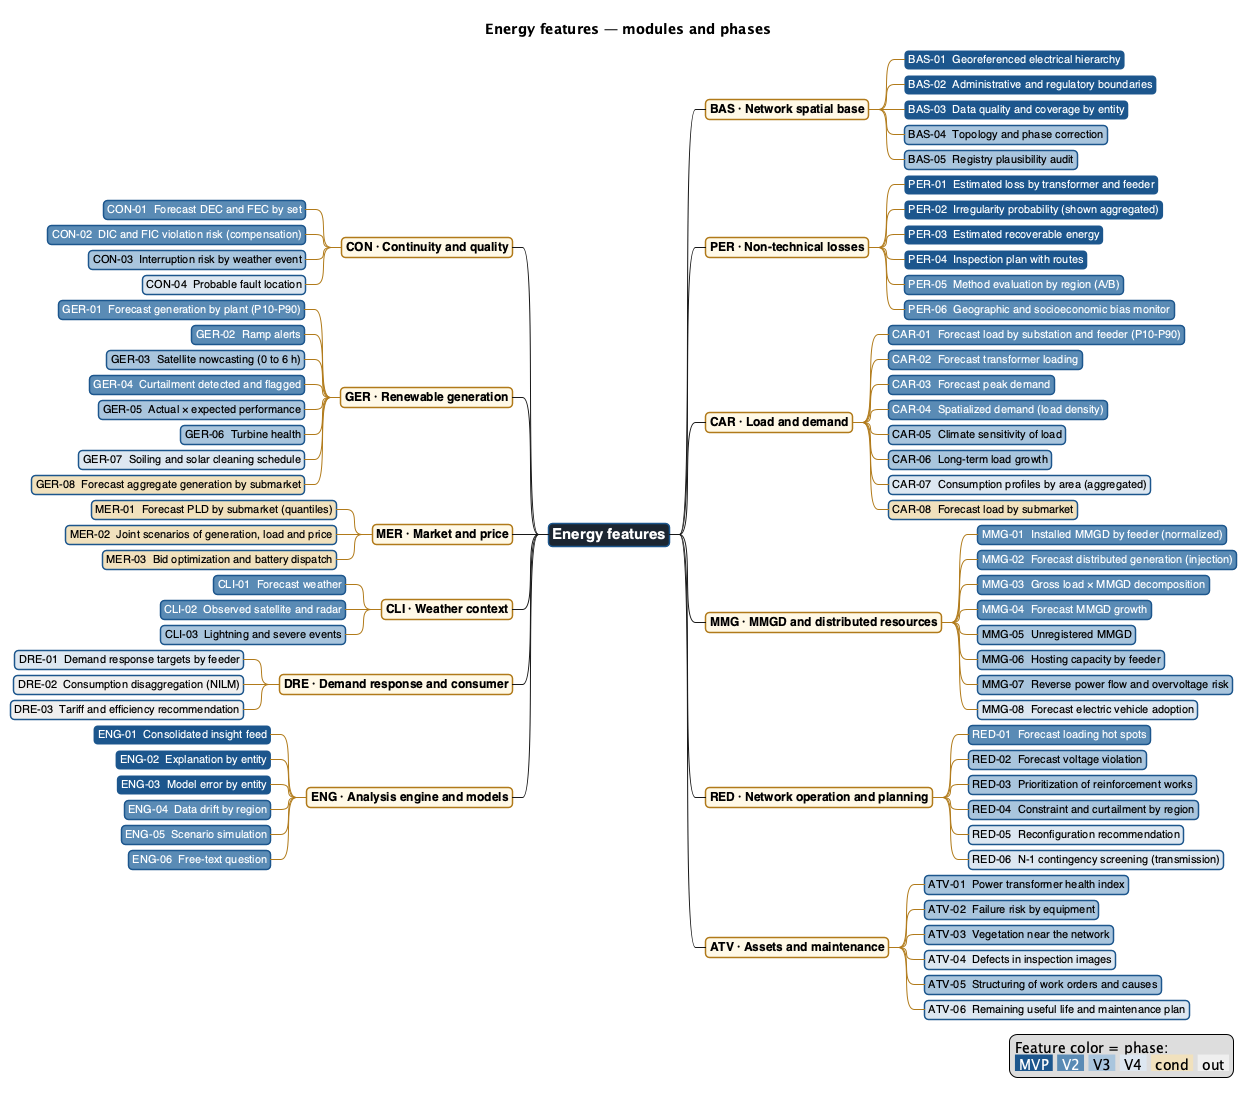
\includegraphics[width=\textwidth]{features-en.png}
\caption{Modules and features, colored by phase.}
\label{fig:mindmap}
\end{figure}

% Generated by features/gerar.py from features/catalogo-en.csv. Do not edit.
\begin{table}[H]\small
\caption{Features by module and phase.}\label{tab:fases}
\begin{tabelalarga}
\begin{tabular}{lccccccc}
\toprule
\textbf{Module} & \textbf{MVP} & \textbf{V2} & \textbf{V3} & \textbf{V4} & \textbf{cond} & \textbf{out} & \textbf{Total} \\
\midrule
BAS \textperiodcentered Network spatial base & 3 & -- & 2 & -- & -- & -- & 5 \\
PER \textperiodcentered Non-technical losses & 4 & 2 & -- & -- & -- & -- & 6 \\
CAR \textperiodcentered Load and demand & -- & 4 & 2 & 1 & 1 & -- & 8 \\
MMG \textperiodcentered MMGD and distributed resources & -- & 4 & 3 & 1 & -- & -- & 8 \\
RED \textperiodcentered Network operation and planning & -- & 1 & 3 & 2 & -- & -- & 6 \\
ATV \textperiodcentered Assets and maintenance & -- & -- & 4 & 2 & -- & -- & 6 \\
CON \textperiodcentered Continuity and quality & -- & 2 & 1 & 1 & -- & -- & 4 \\
GER \textperiodcentered Renewable generation & -- & 3 & 3 & 1 & 1 & -- & 8 \\
MER \textperiodcentered Market and price & -- & -- & -- & -- & 3 & -- & 3 \\
CLI \textperiodcentered Weather context & -- & 2 & 1 & -- & -- & -- & 3 \\
DRE \textperiodcentered Demand response and consumer & -- & -- & -- & 1 & -- & 2 & 3 \\
ENG \textperiodcentered Analysis engine and models & 3 & 3 & -- & -- & -- & -- & 6 \\
\midrule
\textbf{Total} & \textbf{10} & \textbf{21} & \textbf{19} & \textbf{9} & \textbf{5} & \textbf{2} & \textbf{66} \\
\bottomrule
\end{tabular}
\end{tabelalarga}
\end{table}

\begin{table}[H]\footnotesize
\caption{How many features of each module serve each type of client.}\label{tab:clientes}
\begin{tabelalarga}
\begin{tabularx}{\linewidth}{Yccccc}
\toprule
\textbf{Module} & \textbf{Distribution utility} & \textbf{Transmission utility} & \textbf{Generator} & \textbf{Energy trader} & \textbf{Consumer} \\
\midrule
BAS \textperiodcentered Network spatial base & 5 & 2 & 2 & 1 & -- \\
PER \textperiodcentered Non-technical losses & 6 & -- & -- & -- & -- \\
CAR \textperiodcentered Load and demand & 7 & -- & 1 & 1 & -- \\
MMG \textperiodcentered MMGD and distributed resources & 8 & -- & 1 & -- & -- \\
RED \textperiodcentered Network operation and planning & 4 & 2 & 1 & -- & -- \\
ATV \textperiodcentered Assets and maintenance & 6 & 5 & 1 & -- & -- \\
CON \textperiodcentered Continuity and quality & 4 & 1 & -- & -- & -- \\
GER \textperiodcentered Renewable generation & -- & -- & 7 & 2 & -- \\
MER \textperiodcentered Market and price & -- & -- & 3 & 3 & -- \\
CLI \textperiodcentered Weather context & 3 & 3 & 2 & 1 & -- \\
DRE \textperiodcentered Demand response and consumer & 1 & -- & -- & -- & 2 \\
ENG \textperiodcentered Analysis engine and models & 6 & 5 & 5 & 5 & -- \\
\bottomrule
\end{tabularx}
\end{tabelalarga}
\end{table}



% Overall reading of the catalog and the research. Editable text (not generated).
% en-US version of `leitura.tex`: same items, same numbers, same order.

\subsection*{Catalog summary}

\begin{itemize}
  \item \textbf{66 features in 12 modules}: 10 in the MVP, 21 in V2, 19 in V3,
    9 in V4, 5 in the conditional track and 2 out (Table~\ref{tab:fases}).
    That is 59 committed features, 5 held as an option and 2 discarded. 47
    have high map fit, 12 medium and 7 low.
  \item \textbf{The distribution utility concentrates the spatial value}: 50
    of the 66 features serve it (Table~\ref{tab:clientes}). Renewable
    generation and market have medium or low fit, which is consistent with
    the client hypothesis of the specification.
  \item \textbf{CON-01 and CON-02 are in V2}: the BDGD carries monthly DIC and
    FIC per unit. CON-02 (DIC and FIC violation risk) is level 0, has high
    fit and measures the compensation, in reais, paid by the distribution
    utility. CON-01 is a prerequisite of CON-02.
  \item \textbf{The MVP closes the cycle}: base (BAS-01 to 03), losses
    (PER-01 to 04) and engine (ENG-01 to 03) cover feed $\rightarrow$
    diagnosis $\rightarrow$ plan $\rightarrow$ result.
\end{itemize}

\subsection*{Effects of the research on the catalog}

\paragraph{1. Data available at level 0.} With public data alone, there are:
\begin{itemize}
  \item in the BDGD: \textbf{monthly energy per feeder, technical and
    non-technical losses per feeder}, monthly energy, DIC and FIC per unit,
    and the electrical model that ANEEL runs in OpenDSS;
  \item at ANEEL: \textbf{every interruption since 2017 with the feeder and
    substation code}, cause and exclusion; DEC and FEC with limits;
  \item at ONS: generation by plant, half-hourly constrained-off by plant
    with reason and connection point, load with the MMGD share.
\end{itemize}
Therefore, 36 of the 66 features have a level 0 version, among them PER-01
(per feeder), CAR-02, RED-01, CON-01 to 03, GER-01 and GER-04; four of them
(MMG-06, RED-01, RED-02 and ATV-02) depend on a level 1 or level 2 feature.
\textbf{A shadow-mode pilot can be assembled before any client file is
received.}

\paragraph{2. Limits of level 0.}
\begin{itemize}
  \item \textbf{Lag of 8 to 20 months} in the BDGD (2025 edition): it serves
    to assemble the network and to demonstrate, not to operate month by month.
  \item \textbf{The consumer unit is anonymized} (hash) in the public BDGD.
    Linking client data per unit requires the utility's correspondence table;
    through the network (feeder, transformer) the link tends to work.
  \item \textbf{Inconsistent units across utilities} (kWh and MWh in the same
    field) and, in MMGD, injection in place of generation and kW mixed with
    W, observed in two 2025 BDGD files. Normalization per utility and the
    quality layer (BAS-03) are necessary.
  \item The non-technical loss in the two BDGD files is consistent with
    \textbf{accounting apportionment}, not with measurement.
\end{itemize}

\paragraph{3. Three validation rules run through the catalog.}
\begin{itemize}
  \item \textbf{Store what was known at each date}: ONS and CCEE revise data
    after publication, and the ECMWF weather forecast stays available for
    only 2 to 3 days. Archiving from the first day is a requirement.
  \item \textbf{Validate out of space and out of event}: in weather-related
    interruptions, random splits inflate the performance estimate; in Essus
    et al.\ (2026), with spatial and temporal validation, many models do not
    beat the baseline.
  \item \textbf{Control multiple testing} in the engine: entities × layers ×
    detectors require FDR and an alert budget.
\end{itemize}

\paragraph{4. Basis of the exploratory fraction.} Revelas et al.\ (2025) show
that selecting only the most probable targets leads to inconsistent learning;
randomized selection with recorded probabilities allows unbiased estimation
of prevalence, recall, calibration and the selection bias. The same fraction
feeds PER-02, PER-05 and PER-06.

\paragraph{5. Regulatory rules are changing.}
\begin{itemize}
  \item Non-technical loss computed over the measured market since 2025,
    which breaks the series.
  \item Bid-based price formation and two PLDs planned for 2028 (Meta II).
  \item REN 1.098/2024 on MMGD reverse power flow.
  \item Portaria MME 126/2026: 2\% of smart meters per year, prioritizing
    losses.
  \item Proposal for automatic Tarifa Branca.
\end{itemize}
Each one is a drift point to monitor (ENG-04).

\paragraph{6. Licenses to observe.} BDGD under ODbL (share-alike on public
derived databases: consult legal counsel); ECMWF under CC-BY with attribution
on the map; \emph{alibi-detect} under the Business Source License, with a
commercial restriction.

\subsection*{The conditional track}

Five features --- MER-01 to MER-03, CAR-08 and GER-08 --- left the phased
roadmap for the \textbf{cond} track. They are not discarded features: they
are an option on the target-client question that the specification leaves
open (distribution utility, or generator and energy trader). Until that
question is answered, they receive no phase.

Their removal does not affect the others: they form an isolated subtree
---~CAR-08 and GER-08 $\rightarrow$ MER-01 $\rightarrow$ MER-02 $\rightarrow$
MER-03~--- and \textbf{nothing outside it depends on any of the five}. The
external dependencies of the subtree are CLI-01 (of CAR-08) and GER-01 (of
GER-08 and MER-02), features that remain in the roadmap.

Three observations weighed on the decision:
\begin{itemize}
  \item \textbf{It is the part of the generator where the map does not help.}
    The five have low fit, and price by submarket occupies four polygons. If
    the generator track is taken, the spatial anchor is \textbf{RED-04}
    (constraint and curtailment by region): high fit, level 0, no
    dependencies, and already supported by the half-hourly constrained-off
    data from ONS.
  \item \textbf{The premise of MER-03 exists only from 2028.} Bidding only
    makes sense under the hybrid model of the Meta II project, and the first
    battery auction (Portaria MME 136/2026) pays for availability, not free
    arbitrage.
  \item \textbf{The continuity of the source is not guaranteed.} The CCEE
    open data portal has an application firewall; the CKAN endpoint worked on
    September 23, 2026.
\end{itemize}

\subsection*{Dependency chains}

The catalog dependencies define the build order. The main ones in the phased
roadmap:
\begin{itemize}
  \item BAS-01 $\rightarrow$ PER-01, PER-02 $\rightarrow$ PER-03 $\rightarrow$
    PER-04 $\rightarrow$ PER-05, PER-06 (the MVP and its evaluation);
  \item MMG-01 $\rightarrow$ MMG-02 $\rightarrow$ MMG-03, MMG-06, MMG-07;
  \item CAR-01, CAR-02 $\rightarrow$ RED-01 $\rightarrow$ RED-03, DRE-01;
  \item ATV-03 $\rightarrow$ CON-03, and ATV-01, ATV-02 $\rightarrow$ ATV-06.
\end{itemize}

\subsection*{Pending verification}

\begin{enumerate}
  \item BDGD Instruction Manual (not downloaded): official definition of
    energy and losses in CTMT, energy of generating units (injection or
    generation), unit of installed capacity.
  \item Whether the set code in the BDGD matches the one in the DEC and FEC
    indicators.
  \item Whether the distribution utility can reproduce the hash of the unit
    code.
  \item Unit of the value in the CTR typical curves.
  \item Existence of a regulatory obligation to publish hosting capacity.
  \item Legal consultation on the ODbL for derived layers.
\end{enumerate}


% ===========================================================================
% ===========================================================================

\begin{landscape}
\part{Catalog}
\section{Catalog by module}
% Generated by features/gerar.py from features/catalogo-en.csv. Do not edit.
\subsection*{BAS \textperiodcentered{} Network spatial base}
\addcontentsline{toc}{subsection}{BAS \textperiodcentered{} Network spatial base}
\label{cat:BAS}
{\footnotesize\setlength{\tabcolsep}{3pt}
\begin{longtable}{@{}P{1.35cm}P{4.1cm}P{1.3cm}P{3.1cm}P{3.7cm}C{0.6cm}P{3.6cm}P{3.3cm}P{1.1cm}P{0.9cm}P{1.1cm}@{}}
\toprule
\textbf{ID} & \textbf{Feature} & \textbf{Type} & \textbf{Entity} & \textbf{Data} & \textbf{Lvl} & \textbf{Model} & \textbf{Insight / decision} & \textbf{Client} & \textbf{Map} & \textbf{Phase} \\
\midrule\endhead
\textbf{BAS-01} & Georeferenced electrical hierarchy & base & concession, SS, feeder, transformer, CU & BDGD (annual geodatabase, ODbL, 8 to 20 months of lag) & 0 & ETL, graph by connection points, unit normalization per utility & navigate, select & D & \encaixe{3} & \colorbox{fMVP}{\scriptsize \textcolor{white}{\textbf{MVP}}} \\
\textbf{BAS-02} & Administrative and regulatory boundaries & base & state, municipality, census tract, electrical set & IBGE (meshes), ANEEL (sets) & 0 & ETL & cross-reference, filter & D T G & \encaixe{3} & \colorbox{fMVP}{\scriptsize \textcolor{white}{\textbf{MVP}}} \\
\textbf{BAS-03} & Data quality and coverage by entity\newline{\color{black!55}\scriptsize depends on: BAS-01} & layer & all & all ingested sources & 0 & completeness and validity rules & data gap / trigger source, flag layer & D T G C & \encaixe{3} & \colorbox{fMVP}{\scriptsize \textcolor{white}{\textbf{MVP}}} \\
\textbf{BAS-04} & Topology and phase correction\newline{\color{black!55}\scriptsize depends on: BAS-01} & layer & aggregated CU, transformer & smart metering (voltage), BDGD & 3 & voltage series correlation, clustering & registry $\times$ measurement divergence / correct registry & D & \encaixe{3} & \colorbox{fV3}{\scriptsize \textbf{V3}} \\
\textbf{BAS-05} & Registry plausibility audit\newline{\color{black!55}\scriptsize depends on: BAS-01} & insight & aggregated CU, plant & BDGD, ANEEL MMGD registry, reanalysis (NASA POWER) & 0 & physical ceiling (solar resource model), rules & model $\times$ registry divergence / correct registry, audit & D & \encaixe{3} & \colorbox{fV3}{\scriptsize \textbf{V3}} \\
\bottomrule
\end{longtable}}

\subsection*{PER \textperiodcentered{} Non-technical losses}
\addcontentsline{toc}{subsection}{PER \textperiodcentered{} Non-technical losses}
\label{cat:PER}
{\footnotesize\setlength{\tabcolsep}{3pt}
\begin{longtable}{@{}P{1.35cm}P{4.1cm}P{1.3cm}P{3.1cm}P{3.7cm}C{0.6cm}P{3.6cm}P{3.3cm}P{1.1cm}P{0.9cm}P{1.1cm}@{}}
\toprule
\textbf{ID} & \textbf{Feature} & \textbf{Type} & \textbf{Entity} & \textbf{Data} & \textbf{Lvl} & \textbf{Model} & \textbf{Insight / decision} & \textbf{Client} & \textbf{Map} & \textbf{Phase} \\
\midrule\endhead
\textbf{PER-01} & Estimated loss by transformer and feeder\newline{\color{black!55}\scriptsize depends on: BAS-01} & layer & transformer, feeder & BDGD (feeder energy, technical and non-technical losses, energy per unit), client billing, transformer metering where available & 0 & energy balance (feeder energy -- sum of units -- technical), technical loss in OpenDSS, Bayesian hierarchical apportionment among transformers & spatial anomaly, change between cycles / select targets & D & \encaixe{3} & \colorbox{fMVP}{\scriptsize \textcolor{white}{\textbf{MVP}}} \\
\textbf{PER-02} & Irregularity probability (shown aggregated)\newline{\color{black!55}\scriptsize depends on: BAS-01} & layer & CU aggregated by transformer & billing, registry, inspection history & 1 & gradient boosting with neighborhood variables, inverse inspection-propensity weighting, PU learning with propensity (SAR) & concentration / compose plan targets & D & \encaixe{3} & \colorbox{fMVP}{\scriptsize \textcolor{white}{\textbf{MVP}}} \\
\textbf{PER-03} & Estimated recoverable energy\newline{\color{black!55}\scriptsize depends on: PER-01, PER-02} & layer & transformer, feeder, plan & PER-01, PER-02, consumption & 1 & probability $\times$ estimated diverted energy & ranking by value / prioritize & D & \encaixe{3} & \colorbox{fMVP}{\scriptsize \textcolor{white}{\textbf{MVP}}} \\
\textbf{PER-04} & Inspection plan with routes\newline{\color{black!55}\scriptsize depends on: PER-02, PER-03} & decision & selection & PER-02, PER-03, operating base, user constraint & 1 & team orienteering problem (OR-Tools) with randomly drawn exploratory fraction and recorded probabilities & approve and send to the field & D & \encaixe{3} & \colorbox{fMVP}{\scriptsize \textcolor{white}{\textbf{MVP}}} \\
\textbf{PER-05} & Method evaluation by region (A/B)\newline{\color{black!55}\scriptsize depends on: PER-04} & insight & region, batch & inspection results & 1 & A/B test, precision at top-k & method performance / adjust inspection policy & D & \encaixe{2} & \colorbox{fV2}{\scriptsize \textcolor{white}{\textbf{V2}}} \\
\textbf{PER-06} & Geographic and socioeconomic bias monitor\newline{\color{black!55}\scriptsize depends on: PER-04} & insight & census tract, municipality & inspections, IBGE & 1 & flagging rate $\times$ confirmed rate by boundary & unjustified concentration / review criteria & D & \encaixe{3} & \colorbox{fV2}{\scriptsize \textcolor{white}{\textbf{V2}}} \\
\bottomrule
\end{longtable}}

\subsection*{CAR \textperiodcentered{} Load and demand}
\addcontentsline{toc}{subsection}{CAR \textperiodcentered{} Load and demand}
\label{cat:CAR}
{\footnotesize\setlength{\tabcolsep}{3pt}
\begin{longtable}{@{}P{1.35cm}P{4.1cm}P{1.3cm}P{3.1cm}P{3.7cm}C{0.6cm}P{3.6cm}P{3.3cm}P{1.1cm}P{0.9cm}P{1.1cm}@{}}
\toprule
\textbf{ID} & \textbf{Feature} & \textbf{Type} & \textbf{Entity} & \textbf{Data} & \textbf{Lvl} & \textbf{Model} & \textbf{Insight / decision} & \textbf{Client} & \textbf{Map} & \textbf{Phase} \\
\midrule\endhead
\textbf{CAR-01} & Forecast load by substation and feeder (P10--P90)\newline{\color{black!55}\scriptsize depends on: BAS-01, CLI-01} & layer & SS, feeder & SS and feeder metering, weather forecast, calendar & 2 & quantile gradient boosting or TFT, hierarchical reconciliation (MinT) & trend and threshold / schedule operation & D & \encaixe{3} & \colorbox{fV2}{\scriptsize \textcolor{white}{\textbf{V2}}} \\
\textbf{CAR-02} & Forecast transformer loading\newline{\color{black!55}\scriptsize depends on: BAS-01} & layer & transformer & BDGD (monthly energy and curve typology per unit), CTR typical curves (ANEEL), transformer metering where available & 0 & regulatory method (energy $\times$ typical curve in OpenDSS) calibrated on metered transformers & threshold (overload) / transfer load, replace transformer & D & \encaixe{3} & \colorbox{fV2}{\scriptsize \textcolor{white}{\textbf{V2}}} \\
\textbf{CAR-03} & Forecast peak demand\newline{\color{black!55}\scriptsize depends on: CAR-01} & layer & feeder, transformer & measured series & 2 & probabilistic peak forecast by simulation with resampled weather, extreme values & trend and threshold / reinforcement, peak management & D & \encaixe{3} & \colorbox{fV2}{\scriptsize \textcolor{white}{\textbf{V2}}} \\
\textbf{CAR-04} & Spatialized demand (load density)\newline{\color{black!55}\scriptsize depends on: BAS-02} & layer & census tract, grid & BDGD, IBGE, Open Buildings 2.5D, night lights (NASA) & 0 & dasymetric: consumption $\times$ buildings, population and night lights & concentration, change / plan expansion & D & \encaixe{3} & \colorbox{fV2}{\scriptsize \textcolor{white}{\textbf{V2}}} \\
\textbf{CAR-05} & Climate sensitivity of load\newline{\color{black!55}\scriptsize depends on: CAR-01} & layer & feeder, SS & metering, reanalysis, weather forecast & 2 & piecewise regression with degree days, GAM & threshold in heat wave / prepare operation & D & \encaixe{2} & \colorbox{fV3}{\scriptsize \textbf{V3}} \\
\textbf{CAR-06} & Long-term load growth\newline{\color{black!55}\scriptsize depends on: CAR-04} & layer & municipality, feeder & historical consumption, IBGE, EPE (PDE) & 0 & structural models with scenarios & trend / expansion plan & D & \encaixe{3} & \colorbox{fV3}{\scriptsize \textbf{V3}} \\
\textbf{CAR-07} & Consumption profiles by area (aggregated)\newline{\color{black!55}\scriptsize depends on: BAS-01} & layer & transformer, census tract & smart metering or billing & 3 & load curve clustering & profile change / tariffs, campaigns & D & \encaixe{2} & \colorbox{fV4}{\scriptsize \textbf{V4}} \\
\textbf{CAR-08} & Forecast load by submarket\newline{\color{black!55}\scriptsize depends on: CLI-01} & layer & submarket & ONS (verified and scheduled load), weather forecast & 0 & gradient boosting or TFT & trend / contracting & C G & \encaixe{1} & \colorbox{fCond}{\scriptsize \textbf{cond}} \\
\bottomrule
\end{longtable}}

\subsection*{MMG \textperiodcentered{} MMGD and distributed resources}
\addcontentsline{toc}{subsection}{MMG \textperiodcentered{} MMGD and distributed resources}
\label{cat:MMG}
{\footnotesize\setlength{\tabcolsep}{3pt}
\begin{longtable}{@{}P{1.35cm}P{4.1cm}P{1.3cm}P{3.1cm}P{3.7cm}C{0.6cm}P{3.6cm}P{3.3cm}P{1.1cm}P{0.9cm}P{1.1cm}@{}}
\toprule
\textbf{ID} & \textbf{Feature} & \textbf{Type} & \textbf{Entity} & \textbf{Data} & \textbf{Lvl} & \textbf{Model} & \textbf{Insight / decision} & \textbf{Client} & \textbf{Map} & \textbf{Phase} \\
\midrule\endhead
\textbf{MMG-01} & Installed MMGD by feeder (normalized)\newline{\color{black!55}\scriptsize depends on: BAS-01} & context & feeder, transformer & ANEEL MMGD registry (monthly), BDGD & 0 & registry $\times$ BDGD join, unit normalization, module (DC) to inverter (AC) conversion & concentration & D & \encaixe{3} & \colorbox{fV2}{\scriptsize \textcolor{white}{\textbf{V2}}} \\
\textbf{MMG-02} & Forecast distributed generation (injection)\newline{\color{black!55}\scriptsize depends on: MMG-01, CLI-01} & layer & feeder, SS & MMG-01, weather forecast, satellite, metering where available & 0 & forecast irradiance $\times$ installed capacity, calibrated & ramp, reverse power flow threshold / operate the network & D & \encaixe{3} & \colorbox{fV2}{\scriptsize \textcolor{white}{\textbf{V2}}} \\
\textbf{MMG-03} & Gross load $\times$ MMGD decomposition\newline{\color{black!55}\scriptsize depends on: CAR-01, MMG-02} & layer & feeder, SS & CAR-01, MMG-02 & 2 & net load = gross -- MMGD, separate models & steeper duck curve / plan operation & D & \encaixe{3} & \colorbox{fV2}{\scriptsize \textcolor{white}{\textbf{V2}}} \\
\textbf{MMG-04} & Forecast MMGD growth\newline{\color{black!55}\scriptsize depends on: MMG-01} & layer & feeder, municipality & ANEEL MMGD registry, IBGE, PDE 2035 & 0 & hierarchical Bass with spatial covariates, EPE 4MD reference (epe4md) & trend / plan reinforcement & D & \encaixe{3} & \colorbox{fV2}{\scriptsize \textcolor{white}{\textbf{V2}}} \\
\textbf{MMG-05} & Unregistered MMGD\newline{\color{black!55}\scriptsize depends on: MMG-01} & insight & transformer, aggregated CU & billing or smart metering, images & 1 & consumption profile anomaly, rooftop image detection & model $\times$ registry divergence / regularize & D & \encaixe{3} & \colorbox{fV3}{\scriptsize \textbf{V3}} \\
\textbf{MMG-06} & Hosting capacity by feeder\newline{\color{black!55}\scriptsize depends on: MMG-02, CAR-01} & layer & feeder & BDGD electrical model, MMG-02, CAR-01 & 0 & distribution power flow surrogate over scenarios & threshold (no headroom) / approve or deny connections, reinforce & D G & \encaixe{3} & \colorbox{fV3}{\scriptsize \textbf{V3}} \\
\textbf{MMG-07} & Reverse power flow and overvoltage risk\newline{\color{black!55}\scriptsize depends on: MMG-02, CAR-02} & insight & feeder, transformer & MMG-02, CAR-02 & 0 & threshold of forecast injection over minimum load & threshold / adjust tap, reinforce & D & \encaixe{3} & \colorbox{fV3}{\scriptsize \textbf{V3}} \\
\textbf{MMG-08} & Forecast electric vehicle adoption\newline{\color{black!55}\scriptsize depends on: CAR-06} & layer & municipality, feeder & fleet by municipality (Senatran), IBGE & 0 & diffusion model with income and fleet & trend / plan reinforcement & D & \encaixe{3} & \colorbox{fV4}{\scriptsize \textbf{V4}} \\
\bottomrule
\end{longtable}}

\subsection*{RED \textperiodcentered{} Network operation and planning}
\addcontentsline{toc}{subsection}{RED \textperiodcentered{} Network operation and planning}
\label{cat:RED}
{\footnotesize\setlength{\tabcolsep}{3pt}
\begin{longtable}{@{}P{1.35cm}P{4.1cm}P{1.3cm}P{3.1cm}P{3.7cm}C{0.6cm}P{3.6cm}P{3.3cm}P{1.1cm}P{0.9cm}P{1.1cm}@{}}
\toprule
\textbf{ID} & \textbf{Feature} & \textbf{Type} & \textbf{Entity} & \textbf{Data} & \textbf{Lvl} & \textbf{Model} & \textbf{Insight / decision} & \textbf{Client} & \textbf{Map} & \textbf{Phase} \\
\midrule\endhead
\textbf{RED-01} & Forecast loading hot spots\newline{\color{black!55}\scriptsize depends on: CAR-01, CAR-02} & layer & feeder, transformer, SS & BDGD converted to OpenDSS, CAR-01, CAR-02 & 0 & peak quantiles aggregated by topology, flow confirmed in OpenDSS & threshold / transfer load & D & \encaixe{3} & \colorbox{fV2}{\scriptsize \textcolor{white}{\textbf{V2}}} \\
\textbf{RED-02} & Forecast voltage violation\newline{\color{black!55}\scriptsize depends on: CAR-01, MMG-02} & layer & feeder, bus & BDGD electrical model (bdgd2opendss), forecast load and MMGD & 0 & power flow surrogate (GNN), verified by solver & threshold / adjust regulation & D & \encaixe{3} & \colorbox{fV3}{\scriptsize \textbf{V3}} \\
\textbf{RED-03} & Prioritization of reinforcement works\newline{\color{black!55}\scriptsize depends on: RED-01, CAR-06, MMG-06, CON-01, CON-02} & decision & feeder, SS & RED-01, CAR-06, MMG-06 & 1 & optimization under budget: risk $\times$ cost & investment plan & D & \encaixe{3} & \colorbox{fV3}{\scriptsize \textbf{V3}} \\
\textbf{RED-04} & Constraint and curtailment by region & layer & SS, bus & ONS constrained-off by plant (half-hourly, with reason and connection point) & 0 & constraint probability model by region & concentration / site new generation & G T & \encaixe{3} & \colorbox{fV3}{\scriptsize \textbf{V3}} \\
\textbf{RED-05} & Reconfiguration recommendation\newline{\color{black!55}\scriptsize depends on: RED-02} & decision & feeder & electrical model, forecast load & 2 & GNN and optimization, verified by solver & switching & D & \encaixe{2} & \colorbox{fV4}{\scriptsize \textbf{V4}} \\
\textbf{RED-06} & N-1 contingency screening (transmission)\newline{\color{black!55}\scriptsize depends on: RED-02} & layer & line, SS & client network model, forecasts & 2 & GNN surrogate with confirmation by full power flow & threshold / corrective actions & T & \encaixe{2} & \colorbox{fV4}{\scriptsize \textbf{V4}} \\
\bottomrule
\end{longtable}}

\subsection*{ATV \textperiodcentered{} Assets and maintenance}
\addcontentsline{toc}{subsection}{ATV \textperiodcentered{} Assets and maintenance}
\label{cat:ATV}
{\footnotesize\setlength{\tabcolsep}{3pt}
\begin{longtable}{@{}P{1.35cm}P{4.1cm}P{1.3cm}P{3.1cm}P{3.7cm}C{0.6cm}P{3.6cm}P{3.3cm}P{1.1cm}P{0.9cm}P{1.1cm}@{}}
\toprule
\textbf{ID} & \textbf{Feature} & \textbf{Type} & \textbf{Entity} & \textbf{Data} & \textbf{Lvl} & \textbf{Model} & \textbf{Insight / decision} & \textbf{Client} & \textbf{Map} & \textbf{Phase} \\
\midrule\endhead
\textbf{ATV-01} & Power transformer health index\newline{\color{black!55}\scriptsize depends on: BAS-01} & layer & power transformer (SS) & oil reports (DGA), tests, loading & 1 & gradient boosting on dissolved gases, loading and age & change, threshold / inspect, maintain & D T & \encaixe{3} & \colorbox{fV3}{\scriptsize \textbf{V3}} \\
\textbf{ATV-02} & Failure risk by equipment\newline{\color{black!55}\scriptsize depends on: ATV-05} & layer & equipment, feeder & BDGD, interruptions by event (ANEEL), client work orders, weather & 0 & random survival forest, count per km & concentration / preventive maintenance & D & \encaixe{3} & \colorbox{fV3}{\scriptsize \textbf{V3}} \\
\textbf{ATV-03} & Vegetation near the network\newline{\color{black!55}\scriptsize depends on: BAS-01} & layer & feeder section, line & canopy height (Lang 10 m, Meta 1 m), Sentinel-2, client LiDAR & 0 & global canopy height maps, segmentation and height regression & concentration / tree trimming program & D T & \encaixe{3} & \colorbox{fV3}{\scriptsize \textbf{V3}} \\
\textbf{ATV-04} & Defects in inspection images & layer & structure, equipment & drone images & 1 & object detection (YOLO, DETR) & concentration / work order & D T G & \encaixe{3} & \colorbox{fV4}{\scriptsize \textbf{V4}} \\
\textbf{ATV-05} & Structuring of work orders and causes & base & equipment, feeder & free-text work orders & 1 & extraction with a language model & cause concentration & D T & \encaixe{2} & \colorbox{fV3}{\scriptsize \textbf{V3}} \\
\textbf{ATV-06} & Remaining useful life and maintenance plan\newline{\color{black!55}\scriptsize depends on: ATV-01, ATV-02} & decision & equipment & ATV-01, ATV-02 & 1 & survival and optimization under budget and crews & maintenance plan & D T & \encaixe{3} & \colorbox{fV4}{\scriptsize \textbf{V4}} \\
\bottomrule
\end{longtable}}

\subsection*{CON \textperiodcentered{} Continuity and quality}
\addcontentsline{toc}{subsection}{CON \textperiodcentered{} Continuity and quality}
\label{cat:CON}
{\footnotesize\setlength{\tabcolsep}{3pt}
\begin{longtable}{@{}P{1.35cm}P{4.1cm}P{1.3cm}P{3.1cm}P{3.7cm}C{0.6cm}P{3.6cm}P{3.3cm}P{1.1cm}P{0.9cm}P{1.1cm}@{}}
\toprule
\textbf{ID} & \textbf{Feature} & \textbf{Type} & \textbf{Entity} & \textbf{Data} & \textbf{Lvl} & \textbf{Model} & \textbf{Insight / decision} & \textbf{Client} & \textbf{Map} & \textbf{Phase} \\
\midrule\endhead
\textbf{CON-01} & Forecast DEC and FEC by set\newline{\color{black!55}\scriptsize depends on: BAS-02} & layer & electrical set & DEC and FEC by set (ANEEL), interruptions by event with feeder code (ANEEL, since 2017), weather & 0 & time series with weather & threshold against regulatory target / improvement actions & D & \encaixe{3} & \colorbox{fV2}{\scriptsize \textcolor{white}{\textbf{V2}}} \\
\textbf{CON-02} & DIC and FIC violation risk (compensation)\newline{\color{black!55}\scriptsize depends on: CON-01} & layer & feeder, transformer (aggregated) & monthly DIC and FIC per unit in the BDGD, interruptions by event (ANEEL), TUSD & 0 & simulation of DIC, FIC and DMIC per unit and PRODIST compensation rules & ranking by value / prioritize actions & D & \encaixe{3} & \colorbox{fV2}{\scriptsize \textcolor{white}{\textbf{V2}}} \\
\textbf{CON-03} & Interruption risk by weather event\newline{\color{black!55}\scriptsize depends on: CLI-01, CLI-03, ATV-03} & layer & feeder section, line & interruptions by event with cause (ANEEL), weather forecast, lightning (open GLM or BrasilDAT), ATV-03 & 0 & forecast weather $\times$ vulnerability (vegetation, age) & threshold / pre-position crews & D T & \encaixe{3} & \colorbox{fV3}{\scriptsize \textbf{V3}} \\
\textbf{CON-04} & Probable fault location\newline{\color{black!55}\scriptsize depends on: BAS-01} & layer & feeder section & recloser events, smart metering, calls & 3 & classification over reclosers, metering and calls & dispatch crew & D & \encaixe{3} & \colorbox{fV4}{\scriptsize \textbf{V4}} \\
\bottomrule
\end{longtable}}

\subsection*{GER \textperiodcentered{} Renewable generation}
\addcontentsline{toc}{subsection}{GER \textperiodcentered{} Renewable generation}
\label{cat:GER}
{\footnotesize\setlength{\tabcolsep}{3pt}
\begin{longtable}{@{}P{1.35cm}P{4.1cm}P{1.3cm}P{3.1cm}P{3.7cm}C{0.6cm}P{3.6cm}P{3.3cm}P{1.1cm}P{0.9cm}P{1.1cm}@{}}
\toprule
\textbf{ID} & \textbf{Feature} & \textbf{Type} & \textbf{Entity} & \textbf{Data} & \textbf{Lvl} & \textbf{Model} & \textbf{Insight / decision} & \textbf{Client} & \textbf{Map} & \textbf{Phase} \\
\midrule\endhead
\textbf{GER-01} & Forecast generation by plant (P10--P90)\newline{\color{black!55}\scriptsize depends on: CLI-01} & layer & plant & generation by plant from ONS (public), plant SCADA, weather forecast & 0 & gradient boosting or TFT on weather forecast, zero-shot at onboarding & trend / scheduling and declaration & G C & \encaixe{2} & \colorbox{fV2}{\scriptsize \textcolor{white}{\textbf{V2}}} \\
\textbf{GER-02} & Ramp alerts\newline{\color{black!55}\scriptsize depends on: GER-01} & insight & plant, region & GER-01 & 1 & threshold on forecast trajectory & trend and threshold / adjust bid & G & \encaixe{2} & \colorbox{fV2}{\scriptsize \textcolor{white}{\textbf{V2}}} \\
\textbf{GER-03} & Satellite nowcasting (0 to 6 h)\newline{\color{black!55}\scriptsize depends on: CLI-02} & layer & plant, region & GOES-19 & 0 & U-Net on cloud index, latent diffusion (SHADECast) & change / intraday adjustment & G & \encaixe{3} & \colorbox{fV3}{\scriptsize \textbf{V3}} \\
\textbf{GER-04} & Curtailment detected and flagged\newline{\color{black!55}\scriptsize depends on: GER-01} & layer & plant & ONS constrained-off by plant, SCADA & 0 & rules and available power model & concentration / dispute, clean training data & G & \encaixe{2} & \colorbox{fV2}{\scriptsize \textcolor{white}{\textbf{V2}}} \\
\textbf{GER-05} & Actual $\times$ expected performance\newline{\color{black!55}\scriptsize depends on: GER-01} & insight & plant, turbine, solar block & SCADA, resource & 1 & normal behavior model & model $\times$ registry divergence / inspect & G & \encaixe{2} & \colorbox{fV3}{\scriptsize \textbf{V3}} \\
\textbf{GER-06} & Turbine health & layer & turbine & turbine SCADA & 1 & normal behavior model on temperatures and vibration & change / maintenance & G & \encaixe{3} & \colorbox{fV3}{\scriptsize \textbf{V3}} \\
\textbf{GER-07} & Soiling and solar cleaning schedule\newline{\color{black!55}\scriptsize depends on: GER-05} & decision & plant, solar block & SCADA, rain & 1 & estimated soiling loss $\times$ cleaning cost & threshold / schedule cleaning & G & \encaixe{2} & \colorbox{fV4}{\scriptsize \textbf{V4}} \\
\textbf{GER-08} & Forecast aggregate generation by submarket\newline{\color{black!55}\scriptsize depends on: GER-01} & layer & submarket & GER-01, ONS & 0 & aggregation of forecasts & trend / commercial position & C & \encaixe{1} & \colorbox{fCond}{\scriptsize \textbf{cond}} \\
\bottomrule
\end{longtable}}

\subsection*{MER \textperiodcentered{} Market and price}
\addcontentsline{toc}{subsection}{MER \textperiodcentered{} Market and price}
\label{cat:MER}
{\footnotesize\setlength{\tabcolsep}{3pt}
\begin{longtable}{@{}P{1.35cm}P{4.1cm}P{1.3cm}P{3.1cm}P{3.7cm}C{0.6cm}P{3.6cm}P{3.3cm}P{1.1cm}P{0.9cm}P{1.1cm}@{}}
\toprule
\textbf{ID} & \textbf{Feature} & \textbf{Type} & \textbf{Entity} & \textbf{Data} & \textbf{Lvl} & \textbf{Model} & \textbf{Insight / decision} & \textbf{Client} & \textbf{Map} & \textbf{Phase} \\
\midrule\endhead
\textbf{MER-01} & Forecast PLD by submarket (quantiles)\newline{\color{black!55}\scriptsize depends on: CAR-08, GER-08} & layer & submarket & CCEE hourly PLD (annual CSV, CC-BY), NEWAVE/DECOMP/DESSEM decks, ONS & 0 & gradient boosting or DESSEM emulation & trend / commercial position & C G & \encaixe{1} & \colorbox{fCond}{\scriptsize \textbf{cond}} \\
\textbf{MER-02} & Joint scenarios of generation, load and price\newline{\color{black!55}\scriptsize depends on: MER-01, CAR-08, GER-01} & layer & submarket, plant & GER-01, CAR-08, MER-01 & 0 & copulas over marginal forecasts & risk analysis & C G & \encaixe{1} & \colorbox{fCond}{\scriptsize \textbf{cond}} \\
\textbf{MER-03} & Bid optimization and battery dispatch\newline{\color{black!55}\scriptsize depends on: MER-02} & decision & plant, battery & MER-02 & 1 & stochastic optimization over scenarios & bid, dispatch & G C & \encaixe{1} & \colorbox{fCond}{\scriptsize \textbf{cond}} \\
\bottomrule
\end{longtable}}

\subsection*{CLI \textperiodcentered{} Weather context}
\addcontentsline{toc}{subsection}{CLI \textperiodcentered{} Weather context}
\label{cat:CLI}
{\footnotesize\setlength{\tabcolsep}{3pt}
\begin{longtable}{@{}P{1.35cm}P{4.1cm}P{1.3cm}P{3.1cm}P{3.7cm}C{0.6cm}P{3.6cm}P{3.3cm}P{1.1cm}P{0.9cm}P{1.1cm}@{}}
\toprule
\textbf{ID} & \textbf{Feature} & \textbf{Type} & \textbf{Entity} & \textbf{Data} & \textbf{Lvl} & \textbf{Model} & \textbf{Insight / decision} & \textbf{Client} & \textbf{Map} & \textbf{Phase} \\
\midrule\endhead
\textbf{CLI-01} & Forecast weather & context & grid & ECMWF Open Data (CC-BY), GFS, CPTEC/INPE, INMET & 0 & numerical weather prediction with post-processing per entity & -- & D T G C & \encaixe{3} & \colorbox{fV2}{\scriptsize \textcolor{white}{\textbf{V2}}} \\
\textbf{CLI-02} & Observed satellite and radar & context & grid & GOES-19 (ABI), REDEMET and CEMADEN radar & 0 & precipitation nowcasting (pysteps) & -- & D T G & \encaixe{3} & \colorbox{fV2}{\scriptsize \textcolor{white}{\textbf{V2}}} \\
\textbf{CLI-03} & Lightning and severe events & context & grid & BrasilDAT (ELAT/INPE, under contract) or GOES-19 GLM (open) & 0 & -- & -- & D T & \encaixe{3} & \colorbox{fV3}{\scriptsize \textbf{V3}} \\
\bottomrule
\end{longtable}}

\subsection*{DRE \textperiodcentered{} Demand response and consumer}
\addcontentsline{toc}{subsection}{DRE \textperiodcentered{} Demand response and consumer}
\label{cat:DRE}
{\footnotesize\setlength{\tabcolsep}{3pt}
\begin{longtable}{@{}P{1.35cm}P{4.1cm}P{1.3cm}P{3.1cm}P{3.7cm}C{0.6cm}P{3.6cm}P{3.3cm}P{1.1cm}P{0.9cm}P{1.1cm}@{}}
\toprule
\textbf{ID} & \textbf{Feature} & \textbf{Type} & \textbf{Entity} & \textbf{Data} & \textbf{Lvl} & \textbf{Model} & \textbf{Insight / decision} & \textbf{Client} & \textbf{Map} & \textbf{Phase} \\
\midrule\endhead
\textbf{DRE-01} & Demand response targets by feeder\newline{\color{black!55}\scriptsize depends on: CAR-01, RED-01} & decision & feeder & smart metering, program contracts & 3 & counterfactual baseline and load forecast & loading threshold / trigger program & D & \encaixe{3} & \colorbox{fV4}{\scriptsize \textbf{V4}} \\
\textbf{DRE-02} & Consumption disaggregation (NILM) & out & CU & high-frequency metering & 3 & seq2point & -- & I & \encaixe{1} & \colorbox{fFora}{\scriptsize \textbf{out}} \\
\textbf{DRE-03} & Tariff and efficiency recommendation & out & CU & metering, tariffs & 3 & forecast and recommendation & -- & I & \encaixe{1} & \colorbox{fFora}{\scriptsize \textbf{out}} \\
\bottomrule
\end{longtable}}

\subsection*{ENG \textperiodcentered{} Analysis engine and models}
\addcontentsline{toc}{subsection}{ENG \textperiodcentered{} Analysis engine and models}
\label{cat:ENG}
{\footnotesize\setlength{\tabcolsep}{3pt}
\begin{longtable}{@{}P{1.35cm}P{4.1cm}P{1.3cm}P{3.1cm}P{3.7cm}C{0.6cm}P{3.6cm}P{3.3cm}P{1.1cm}P{0.9cm}P{1.1cm}@{}}
\toprule
\textbf{ID} & \textbf{Feature} & \textbf{Type} & \textbf{Entity} & \textbf{Data} & \textbf{Lvl} & \textbf{Model} & \textbf{Insight / decision} & \textbf{Client} & \textbf{Map} & \textbf{Phase} \\
\midrule\endhead
\textbf{ENG-01} & Consolidated insight feed & insight & whole hierarchy & all layers & 0 & LISA and Getis-Ord with FDR, change points, impact $\times$ significance score, consolidation & all detectors / follow insight & D T G C & \encaixe{3} & \colorbox{fMVP}{\scriptsize \textcolor{white}{\textbf{MVP}}} \\
\textbf{ENG-02} & Explanation by entity & layer & all & models & 0 & variable importance (SHAP) & -- & D T G C & \encaixe{3} & \colorbox{fMVP}{\scriptsize \textcolor{white}{\textbf{MVP}}} \\
\textbf{ENG-03} & Model error by entity & layer & all & actuals & 1 & forecast $\times$ actual (nMAE, CRPS, precision at top-k) & model performance / recalibrate, distrust & D T G C & \encaixe{3} & \colorbox{fMVP}{\scriptsize \textcolor{white}{\textbf{MVP}}} \\
\textbf{ENG-04} & Data drift by region & insight & all & model inputs & 1 & two-sample tests (KS, PSI, MMD) with effect size and FDR & change / retrain & D T G C & \encaixe{2} & \colorbox{fV2}{\scriptsize \textcolor{white}{\textbf{V2}}} \\
\textbf{ENG-05} & Scenario simulation & decision & selection & layers & 0 & models with altered inputs & compare alternatives & D & \encaixe{3} & \colorbox{fV2}{\scriptsize \textcolor{white}{\textbf{V2}}} \\
\textbf{ENG-06} & Free-text question\newline{\color{black!55}\scriptsize depends on: ENG-01} & decision & selection & layers and insights & 0 & language model orchestrating queries, numbers come from the engine & -- & D T G C & \encaixe{3} & \colorbox{fV2}{\scriptsize \textcolor{white}{\textbf{V2}}} \\
\bottomrule
\end{longtable}}


\end{landscape}

% ===========================================================================
\part{Research by module}
% ===========================================================================

% Research cards: BAS, PER
% Checked on the web on September 23, 2026, with two 2025 BDGD (V11) actually opened.
% "(to be confirmed)" marks what was not verified in a source or in data.

\section{Network spatial base and non-technical losses}

\subsection*{Inside the BDGD}

Two 2025 BDGD (version V11) were downloaded and opened for this research
[2]. The Instruction Manual could not be downloaded (the item on the portal
responds with an error), so the semantics of some fields were inferred from the
order of magnitude of the values, and this is indicated.

\paragraph{Access.} ANEEL Open Data, ODbL license, annual update
[1]. One geodatabase per distribution utility on the ANEEL ArcGIS Hub, listable
through a search API and downloadable \textbf{without authentication} [2]. 2025
sizes: from about 1~MB (cooperatives) to 4~GB (Cemig-D). The ODbL has a
share-alike clause for derived databases used publicly:
validate with legal counsel whether the product layers fall under it (to be confirmed).

\paragraph{Lag.} In a 2025 BDGD, the period runs from January to
December 2025, with extraction in May and publication in August 2026: in that
edition, publication occurred \textbf{8 to 20 months} after the reference
month. The public data serve to
build the network and the pilot, not for monthly operation.

\begin{table}[H]
\centering\small
\caption{BDGD entities relevant to the catalog.}
\begin{tabularx}{\textwidth}{P{3.2cm} L}
\toprule
\textbf{Entity} & \textbf{What it carries (verified in the files)} \\
\midrule
CTMT (feeder) & substation, voltages, HV transformer; \textbf{monthly circuit energy} (ENE\_01 to 12, compatible with injected energy, to be confirmed); \textbf{technical losses} by segment and transformation (PERD\_*); \textbf{monthly non-technical losses} at medium and low voltage (PNTMT, PNTBT) \\
UNTRMT (transformer) & rated power, iron and total losses, feeder, substation, electrical set, municipality, phases, connection date \\
UCBT, UCMT (units) & no geometry of their own; link to the point (PONNOT) and to the transformer with 100\% fill rate in the sample; class, CNAE, load-curve typology, installed load, DG code, \textbf{monthly energy, DIC and FIC}; MV also with demand. \textbf{The unit code is a 64-character hash} \\
BE, EP, PT, PNT & energy balance, pass-through energy, monthly technical and non-technical losses of the distribution utility \\
CONJ, ARAT, SUB & polygons of electrical set, service area and substation (the latter came empty in one of the files) \\
SSDMT, SSDBT & network segments, with connection points to build the graph \\
\bottomrule
\end{tabularx}
\end{table}

\paragraph{Pitfalls verified in the data.}
\begin{itemize}
  \item \textbf{Different units across distribution utilities}: feeder
    energy appears in kWh in one and in MWh in the other, and within a single
    table there are fields on different scales. Every loss/energy ratio must
    be normalized by distribution utility and by field, or the naive calculation gives
    ``technical loss of 250\%''.
  \item \textbf{The BDGD non-technical loss appears to be apportionment}: round values
    that match the aggregate table indicate accounting allocation, not
    measurement (to be confirmed in the Manual).
  \item \textbf{Implausible MMGD}: in a distribution utility in SC, annual energy
    over installed power reaches 4,470~kWh/kW/year, incompatible with
    photovoltaic generation (median 900), which is compatible with the
    injection and unit problems.
  \item \textbf{Codes}: feeder, transformer and connection points
    appear to be operational codes, but the consumer unit is anonymized.
    Linking client data \emph{by unit} requires the distribution utility to
    provide the mapping; linking \emph{through the network} tends to work (to be
    confirmed with a client).
\end{itemize}

\paragraph{ANEEL loss indicators [5--8].} In 2024, total loss was
about 14\% of injected energy: technical 7.4\% (44.6~TWh) and non-technical
6.6\% (40.2~TWh). The ten largest distribution utilities account for 74\% of the
non-technical loss; Light and Amazonas Energia, 34\%. The cost of the actual non-technical loss was
estimated by ANEEL at R\$~10.3 billion. The regulatory limit comes from PRORET Submódulo
2.6 through benchmarking of socioeconomic complexity [9]. \textbf{Since 2025,
non-technical loss has been calculated on the measured market, no longer the
billed one} (Despacho 1.220/2025), which breaks the historical series. The regulatory
technical loss is calculated by ANEEL by building the BDGD in OpenDSS [12].

% ---------------------------------------------------------------------------
\subsection{BAS \textperiodcentered{} Network spatial base}

\begin{ficha}{BAS-01 \textperiodcentered{} Georeferenced electrical hierarchy}{MVP}
\campo{Data} BDGD: substation, feeder (CTMT), transformer (UNTRMT),
units (UCBT, UCMT) and their points (PONNOT); segments (SSDMT, SSDBT) for
connectivity. Converters to OpenDSS: \emph{bdgd-tools} and
\emph{bdgd2dss} [11].
\campo{Approaches} Baseline: ETL with GDAL to GeoParquet or PostGIS.
Recommended: graph from the connection points with validation of radiality and
reachability from the feeder head; unit normalization
by distribution utility; composite key (distribution utility, code); versioning by
base year.
\campo{Metrics} Percentage of units linked to transformer, point and
feeder; reachable segments; loops per circuit; divergence between
years.
\campo{Pitfalls} Substation polygon may come empty; files of several
GB; resubmissions with different dates; the BDGD is a simplified model of the network
[1].
\end{ficha}

\begin{ficha}{BAS-02 \textperiodcentered{} Administrative and regulatory boundaries}{MVP}
\campo{Data} IBGE, 2022 tract mesh and aggregates [13]; the municipality in the
BDGD uses the 7-digit IBGE code; electrical sets in the CONJ polygon of the
BDGD and in the continuity indicators [14].
\campo{Approaches} Bridge table unit, tract, municipality, set,
computed once by spatial join.
\campo{Pitfalls} 2010 and 2022 tracts incompatible; sets change
between years; matching the BDGD set code with that of the indicators (to be
confirmed).
\end{ficha}

\begin{ficha}{BAS-03 \textperiodcentered{} Data quality and coverage by entity}{MVP}
\campo{Typical BDGD problems} Disconnected sections, inconsistent
buses, wrong links, incorrect phase, inadequate impedances,
misallocated load; a single parameterization error changed the calculated technical
loss by up to 1.45\% [12].
\campo{Approaches} Completeness and validity rules by field (Great
Expectations, pandera) and a \textbf{score by entity} with physical rules
(total loss greater than iron loss; yield below the cap; loss
smaller than energy), consistency rules (sum of the units smaller than the feeder
energy), unit detection by order of magnitude and missing links.
The score becomes a layer and qualifies the others.
\campo{Pitfalls} Rules calibrated on one distribution utility fail on another because
of the units; the quality layer can be read as an accusation against the
client.
\end{ficha}

\begin{ficha}{BAS-04 \textperiodcentered{} Topology and phase correction}{V3}
\campo{Data} Voltage series from smart meters (level 3) and the BDGD.
Portaria Normativa MME 126/2026 mandates additional deployment in 2\% of
units per year for 24 months starting in March 2026, prioritizing reduction
of non-technical loss [17].
\campo{Approaches} Baseline: correlation of the voltage series.
Recommended: clustering on voltage correlation with a transformer capacity
constraint, generating candidates for field validation
(Short 2013 [19]; Hoogsteyn et al.\ 2022: voltage series outperform
power series [20]).
\campo{Pitfalls} Sparse coverage per transformer; synchronization between
meters; MMGD alters the voltage profile.
\end{ficha}

\begin{ficha}{BAS-05 \textperiodcentered{} Registry plausibility audit}{V3}
\campo{Data} BDGD generating units (power, energy, DG code);
ANEEL MMGD registry [15]; NASA POWER [16].
\campo{Approaches} Baseline: annual yield cap by municipality
from irradiation. Recommended: expected monthly range from a physical model
(pvlib), compared with the recorded injection, which is a lower bound on generation;
cross-check the BDGD power against the registry to detect W and kW. Real example:
4,470~kWh/kW/year in SC.
\campo{Pitfalls} Injection depends on self-consumption: the test works as a cap,
not as a floor; remote compensation; missing DG code.
\end{ficha}

% ---------------------------------------------------------------------------
\subsection{PER \textperiodcentered{} Non-technical losses}

\begin{ficha}{PER-01 \textperiodcentered{} Estimated loss by transformer and feeder}{MVP}
\campo{Data} Public: feeder energy, technical and non-technical losses
from CTMT, energy by unit, iron and total losses of the transformers.
Client: monthly billing (the BDGD is annual and lagged) and transformer
metering when available.
\campo{Approaches} \textbf{Baseline by feeder, with public data
only}: feeder energy minus the sum of the units (LV, MV,
public lighting) minus injected generation, compared with the BDGD
losses. By transformer without metering: technical loss from iron plus
copper proportional to the square of the load; the non-technical loss is left as the residual.
Recommended: power flow in OpenDSS for the technical loss (as ANEEL does)
and balance for the total, with a Bayesian hierarchical model that splits the
feeder residual among the transformers using the attributes from
PER-02. Recent literature: technical loss without power flow from
sparse voltage [41]; estimation of rates by region in a Brazilian city
[43].
\campo{Metrics} Error against metered transformers; stability between
cycles; agreement with the regulatory total.
\campo{Pitfalls} Mixed units; BDGD non-technical loss appears to be apportionment;
billing cycle different from the calendar month; estimated public lighting;
energy injected by DG enters the balance.
\end{ficha}

\begin{ficha}{PER-02 \textperiodcentered{} Irregularity probability}{MVP}
\campo{Data} Client: inspections with outcome (positive and negative),
billing, meter replacements, disconnections. BDGD: class, CNAE, installed load,
DIC and FIC, DG code. Context: census tract, transformer loss
(PER-01), neighborhood.
\campo{Approaches} Baseline: rules and gradient boosting on the
inspections. Recommended: boosting with \textbf{neighborhood variables} [23],
selection bias correction by inverse inspection propensity weighting,
calibration on the exploratory fraction and PU learning.
\campo{What the literature says} Glauner et al.\ showed covariate shift in a
Brazilian dataset of 3.6 million clients and 820 thousand inspections: inspections
concentrated in neighborhoods and classes make the models biased [22,24].
Coma-Puig and Carmona propose measuring recovered energy and explaining [25,26].
Revelas, Boldea and Werker (2025) show that selecting only the most probable
leads to inconsistent learning and that randomized selection allows
updating the model as if the sample were random [35]: this is the basis
adopted for the exploratory fraction. In PU learning [31--33], the assumption that the
labeled positives were chosen at random \textbf{does not hold} in losses,
because inspections are targeted: use variants with propensity dependent
on the variables (SAR-PU) [34].
\campo{Brazilian cases} Light: satellite and BDGD for illegal connections
[37], ANEEL R\&D with GESEL/UFRJ on areas with severe operating
restrictions [39]; Optimum-Path Forest (UNESP, Unicamp) [28]; survey of
28 experts [36]; irrigators in RS [44].
\campo{Metrics} Precision at top-k with $k$ equal to the inspection capacity;
energy-weighted recall; calibration \textbf{measured on the exploratory
fraction}; AUC only as a diagnostic.
\campo{Pitfalls} Metrics inflated by oversampling and leakage; inspection
negative is noisy; drift after meter replacement; LGPD.
\end{ficha}

\begin{ficha}{PER-03 \textperiodcentered{} Estimated recoverable energy}{MVP}
\campo{Approaches} Baseline: probability × estimated diverted energy
(consumption before the drop or median of the peers). Recommended: two stages,
probability × severity, with severity regressed on the confirmed
positives, optimizing net return (recovered minus inspection
cost), as in Massaferro, Di Martino and Fernández (UTE, Uruguay) [27].
\campo{Pitfalls} Severity is observed only in the positives (another bias);
accounting recovery is not sustained recovery; double counting with the
transformer balance.
\end{ficha}

\begin{ficha}{PER-04 \textperiodcentered{} Inspection plan with routes}{MVP}
\campo{Approaches} Baseline: top by expected value and nearest-neighbor
route. Recommended: \textbf{team orienteering problem} (routing with
prizes) maximizing expected value under each team's work shift, solved
with OR-Tools; \textbf{exploratory fraction drawn at random by stratum with
recorded probabilities} (5 to 15\%) [35], used later as weights in
PER-02, PER-05 and PER-06. No specific literature on
routing for losses was found.
\campo{Metrics} Value captured over the optimum; inspections per team and day;
cost per productive inspection; percentage of the plan executed.
\campo{Pitfalls} Safety criteria take precedence over the random draw;
teams that do not follow the random draw; grouping targets by route reintroduces geographic bias.
\end{ficha}

\begin{ficha}{PER-05 \textperiodcentered{} Method evaluation by region (A/B)}{V2}
\campo{Approaches} Randomization \textbf{by cluster} (transformer, neighborhood
or team) to avoid contamination; random arm as the prevalence
reference; Horvitz--Thompson estimators; effect measured in recovered
energy and in feeder loss over time (difference in
differences).
\campo{Pitfalls} Low statistical power with low prevalence; deterrence
effect among neighbors; change of the regulatory metric in 2025.
\end{ficha}

\begin{ficha}{PER-06 \textperiodcentered{} Geographic and socioeconomic bias monitor}{V2}
\campo{Approaches} Compare, by breakdown, the flagging rate with the
confirmation rate \textbf{estimated on the random fraction}; calibration and true
positive rate by group; proportion tests with correction for
multiple comparisons; Bayesian smoothing in small tracts. No
specific work on fairness in losses in Brazil was found.
Regulation recognizes socioeconomic complexity as a determinant, so
different prevalences are expected [6].
\campo{Pitfalls} Without a random arm, bias cannot be separated from real
prevalence; re-identification in fine breakdowns; using income as a variable and auditing
the same variable.
\end{ficha}

\subsection*{References for this section}
{\small
\begin{enumerate}[label={[\arabic*]},leftmargin=2.2em,itemsep=1pt]
\item ANEEL, BDGD: \url{https://dadosabertos.aneel.gov.br/dataset/base-de-dados-geografica-da-distribuidora-bdgd}
\item ANEEL ArcGIS Hub, search API: \url{https://dadosabertos-aneel.opendata.arcgis.com/}
\item BDGD Instruction Manual (not downloaded)
\item ANEEL, PRODIST Módulos 7 and 10
\item ANEEL, Perdas de Energia: \url{https://www.gov.br/aneel/pt-br/assuntos/distribuicao/perdas-de-energia}
\item ANEEL/STR, Perdas de Energia Elétrica na Distribuição (2025, base year 2024)
\item ANEEL, Luz na Tarifa dashboard, losses: \url{https://portalrelatorios.aneel.gov.br/luznatarifa/perdasenergias}
\item ANEEL, tariffs and economic and financial information
\item ANEEL, PRORET Submódulo 2.6
\item ANEEL, losses report (2026)
\item bdgd-tools: \url{https://github.com/eniocc/bdgd-tools}; bdgd2dss: \url{https://github.com/ArthurGS97/bdgd2dss}
\item Norven, BDGD quality and technical loss calculation
\item IBGE, census tract mesh
\item ANEEL, collective continuity indicators
\item ANEEL, MMGD installations
\item NASA POWER, daily API: \url{https://power.larc.nasa.gov/docs/services/api/temporal/daily/}
\item Portaria Normativa MME 126/2026
\item Enel SP, smart meters (to be confirmed)
\item Short (2013), \emph{IEEE Trans.\ Smart Grid} 4(2):651--658
\item Hoogsteyn et al.\ (2022): \url{https://arxiv.org/abs/2204.06372}
\item Glauner et al.\ (2017), survey, \emph{IJCIS}: \url{https://arxiv.org/abs/1606.00626}
\item Glauner et al.\ (2017), ISAP: \url{https://arxiv.org/abs/1702.03767}
\item Glauner et al.\ (2016), neighborhood, BDCAT: \url{https://arxiv.org/abs/1607.00872}
\item Glauner, Valtchev and State (2018), ESANN
\item Coma-Puig and Carmona (2019), \emph{Energies} 12(9):1748
\item Coma-Puig and Carmona (2022), \emph{Machine Learning}, doi:10.1007/s10994-021-06051-1
\item Massaferro, Di Martino and Fernández, \emph{IEEE TPWRS}, doi:10.1109/TPWRS.2019.2928276
\item Ramos, Souza, Papa and Falcão, OPF; Passos Júnior et al.\ (2016), \emph{EPSR} 140
\item Messinis and Hatziargyriou (2018), \emph{EPSR} 158
\item Zheng et al.\ (2018), \emph{IEEE TII} 14(4)
\item Elkan and Noto (2008), KDD
\item Kiryo et al.\ (2017), nnPU: \url{https://arxiv.org/abs/1703.00593}
\item Bekker and Davis (2020), \emph{Machine Learning} 109: \url{https://arxiv.org/abs/1811.04820}
\item SAR-PU (KU Leuven): \url{https://github.com/ML-KULeuven/SAR-PU}
\item Revelas, Boldea and Werker (2025): \url{https://arxiv.org/abs/2509.18739}
\item Savian et al.\ (2022), \emph{IJEEP} 12(3)
\item Gremes et al.\ (2024), NTL-Unet, \emph{Sensors} 24:4924
\item Assignment of buildings to units, SEGAN (2024)
\item GESEL/UFRJ and Light, ANEEL R\&D
\item Cenário Energia, Light (August 2026)
\item Bariya and Flaspohler (2025): \url{https://arxiv.org/abs/2506.21311}
\item Nguyen et al.\ (2023), \emph{Big Data}
\item Non-technical loss rates by region, \emph{EPSR} (2023)
\item Losses among irrigators, \emph{Energies} 16:6832 (2023)
\end{enumerate}}

% Research cards: CAR, MMG
% Checked on the web on September 23, 2026. "(to be confirmed)" marks what was not verified in a source.

\section{Load, demand and MMGD}

\subsection*{Shared sources}

\begin{table}[H]
\centering\small
\caption{Sources shared by the CAR and MMG modules.}
\begin{tabularx}{\textwidth}{P{3.2cm} L P{4.2cm}}
\toprule
\textbf{Source} & \textbf{What it provides} & \textbf{Pitfalls} \\
\midrule
BDGD (ANEEL) [1,2] & annual geodatabase by distribution utility, reference date December 31, published about 8 months after the reference date in the 2025 edition. In the unit tables: feeder, transformer, substation, municipality, class, CNAE, curve typology, monthly energy and demand, \textbf{monthly DIC and FIC}, DG code and coordinates & the open CSVs only carry \textbf{legal entities}; residential requires the full geodatabase. DG energy as injection and power in kW and W mixed: observed empirically in a subset, not confirmed in the specification \\
MMGD registry (ANEEL) [4,5] & monthly; municipality, substation and approximate coordinates, modality (local, remote, shared), class, source, power in kW & power is the sum of the \textbf{modules} (DC), not of the inverter; there is no feeder, only substation \\
CTR typical curves (ANEEL) [6] & typical consumer and typical network from the measurement campaigns of the tariff reviews, by day type, in 15-minute intervals & unit of the value not stated; each distribution utility has one campaign year; curves predate the MMGD expansion \\
ONS, verified and scheduled load [7,8] & half-hourly by load area, with components, including the \textbf{share served by MMGD} & breaks in 2021 (global load) and 2023 (estimated MMGD enters the load) [9]; ONS advises not using years before 2022 [10] \\
IBGE, 2022 Census [11,12] & aggregates and census tract mesh & 2010 and 2022 tracts are not comparable without harmonization \\
Nighttime lights (NASA Black Marble) [13,14] & 500~m, daily, monthly and annual & public lighting is not consumption; urban saturation \\
Google Open Buildings 2.5D Temporal [15] & building presence, count and height, annual from 2016 to 2023, covers Brazil & raster, no polygon; ends in 2023 \\
Senatran, fleet [16,17] & monthly by municipality and fuel since 2003 & fleet registered at the owner's domicile; rental companies concentrate registrations \\
EPE [18--21] & PDE 2035 (MMGD, electromobility, demand); the 4MD model and the R package \emph{epe4md} & national or by distribution utility; the disaggregation is the user's \\
\bottomrule
\end{tabularx}
\end{table}

% ---------------------------------------------------------------------------
\subsection{CAR \textperiodcentered{} Load and demand}

\begin{ficha}{CAR-01 \textperiodcentered{} Forecast load by substation and feeder}{V2}
\campo{Data} Substation and feeder metering at 15 minutes (client);
weather forecast and reanalysis; calendar; BDGD topology; MMGD by
feeder (MMG-01).
\campo{Approaches} Baseline: similar profile and regression with
temperature and calendar (Tao Vanilla style) [22]. Recommended: one
global quantile boosting model for all feeders (P10, P50, P90),
followed by hierarchical reconciliation transformer, feeder,
substation, area with MinT [23]; probabilistic version as in Ben Taieb et
al.\ with smart meters [24]. Recent literature: TFT [26] and foundation
models [27--30]; \textbf{Chronos-2} accepts native covariates,
needed for weather [28]; use as challenger and for feeders with
little history [31,32].
\campo{Metrics} Pinball and CRPS [33]; P10--P90 coverage (expected 80\%);
WAPE of the P50 by horizon; zero-sum residual after reconciling.
\campo{Pitfalls} Switching operations and transfers create false steps (requires
a switching log); what is metered is net load; MinT with thousands of series needs
covariance with shrinkage.
\end{ficha}

\begin{ficha}{CAR-02 \textperiodcentered{} Forecast transformer loading}{V2}
\campo{Data} BDGD: monthly energy and curve typology by unit, link
to the transformer and rated power [1]; CTR curves [6]; weather; sample
metering of the client's transformers, when available.
\campo{Approaches} Baseline: the \textbf{regulatory method} for technical
losses, which ANEEL has run in OpenDSS since 2014 from the BDGD, with
monthly energy × typical curves in 24 levels [34,35]. Recommended: the
baseline plus a calibration factor learned on metered transformers
(boosting with class composition, number of units, weather and MMGD), to
reduce the underestimation of diversity; output as peak distribution and
probability of exceeding 100\% or 120\%. Conversion to OpenDSS:
\emph{bdgd2dss} [36].
\campo{Metrics} Peak error on metered transformers; AUC-PR of
overload; Brier.
\campo{Pitfalls} CTR curves old and without MMGD [3]; wrong unit to
transformer link in the BDGD; rated power is not thermal capacity.
\end{ficha}

\begin{ficha}{CAR-03 \textperiodcentered{} Forecast peak demand}{V2}
\campo{Approaches} Baseline: historical maximum × growth.
Recommended: peak density forecast by simulation, feeding the
hourly model with many years of resampled weather and extracting the
10, 50 and 90\% exceedance probabilities (Hyndman and Fan [37]; Hong, Wilson
and Xie [38]). Recent literature: extreme values (GEV, GPD) on residuals.
\campo{Metrics} Pinball at the high quantiles; error of the peak value and
time; hit rate of ``peak day''.
\campo{Pitfalls} With MMGD the net peak shifts to the early evening;
few extremes in the history.
\end{ficha}

\begin{ficha}{CAR-04 \textperiodcentered{} Spatialized demand}{V2}
\campo{Data} Consumption by unit with coordinates (full BDGD or
client); 2022 Census tracts; Open Buildings 2.5D; Black Marble.
\campo{Approaches} Baseline: direct aggregation of units into a hexagonal
grid or tract, where there are coordinates. Recommended: dasymetric in
WorldPop style, with a random forest that predicts consumption density from built
area and volume, population, nighttime light and land use, redistributing the
known total with a sum constraint [39,40]. Recent literature:
downscaling with deep learning at about 130~m [41].
\campo{Metrics} Spatial cross-validation (municipality left out)
against the actual aggregation; exact mass conservation.
\campo{Pitfalls} Nighttime light measures lighting; \textbf{LGPD}: aggregate with
a minimum number of units per cell.
\end{ficha}

\begin{ficha}{CAR-05 \textperiodcentered{} Climate sensitivity of load}{V3}
\campo{Approaches} Baseline: piecewise regression with degree days; the
slope above the balance point (MW/°C) is the indicator. Recommended:
GAM with temperature spline, hour × temperature interaction, lagged
effects from 24 to 72~h and Bayesian hierarchy across feeders. State of the
art: distributional regression [42]. Context: the IEA estimates +3.6~GW of demand
per +1~°C in Brazil [43,44].
\campo{Pitfalls} Estimate on gross load (a hot, sunny day reduces
the net load); air-conditioning penetration changes the sensitivity over the years.
\end{ficha}

\begin{ficha}{CAR-06 \textperiodcentered{} Long-term load growth}{V3}
\campo{Approaches} Baseline: PDE rate applied top-down
[45]. Recommended: structural model by class with scenarios, reconciled with
the PDE at the top, and spatial allocation by built-area growth;
large point loads (data centers, industry) as events.
\campo{Metrics} Rolling-origin backtest over 3 to 10 years; spatial
allocation error; scenario coverage.
\end{ficha}

\begin{ficha}{CAR-07 \textperiodcentered{} Consumption profiles by area}{V4}
\campo{Approaches} Without smart metering, synthetic profile from the class
composition and CTR curves; with metering, clustering (k-medoids with DTW, GMM)
evaluated by Chicco's indices [46].
\campo{Pitfalls} A synthetic profile only reproduces the existing typologies;
LGPD in small aggregations.
\end{ficha}

\begin{ficha}{CAR-08 \textperiodcentered{} Forecast load by submarket}{cond}
\campo{Approaches} Baseline: the ONS scheduled load [8].
Recommended: boosting or TFT by subsystem with load-weighted weather and the
MMGD component modeled separately [7]; reconciliation area, subsystem, SIN.
\campo{Pitfalls} Breaks of 2021 and 2023 [9]; retroactive revisions.
\end{ficha}

% ---------------------------------------------------------------------------
\subsection{MMG \textperiodcentered{} MMGD and distributed resources}

\begin{ficha}{MMG-01 \textperiodcentered{} Installed MMGD by feeder}{V2}
\campo{Approach} (1) Join registry and BDGD by the DG code; on failure,
spatial join within the same substation. (2) Normalize units by
comparing with the registry power (a ratio close to 1,000 indicates W). (3)
For the network what counts is the plant location, not the unit that receives the credit
(remote, shared). (4) Convert modules (DC) to inverter (AC) with the
sizing factor used by EPE [20].
\campo{Metrics} Join rate; power divergence between sources by
feeder.
\campo{Pitfalls} BDGD with 8 to 20 months of lag and monthly registry: use the
registry for counts and the BDGD for topology; approximate coordinates lead
to the wrong feeder in dense areas.
\end{ficha}

\begin{ficha}{MMG-02 \textperiodcentered{} Forecast distributed generation}{V2}
\campo{Approaches} Baseline: installed power × irradiance × PR (0.75
local and 0.80 remote, 4MD assumptions) [20]. Recommended: physical model with
pvlib and upscaling by reference systems, with quantile
post-processing calibrated on the feeder metering. ONS estimates MMGD with
the ANEEL capacity, INPE irradiation and its own capacity factor [9].
\campo{Generation and injection} Generation is not injection: injection is generation minus
simultaneous self-consumption, which requires a model of the unit's load.
\campo{Pitfalls} Unknown orientation; unregistered capacity;
inverter limiting.
\end{ficha}

\begin{ficha}{MMG-03 \textperiodcentered{} Gross load × MMGD decomposition}{V2}
\campo{Approaches} Baseline: add the estimated generation to the net load.
Recommended: joint estimation, net = load(weather, calendar) $-\,k$ ×
PV proxy(irradiance), with $k$ (effective power) by regression or Kalman
filter; the estimated $k$ audits the registry and feeds MMG-05. References:
SunDance [48], unsupervised disaggregation [49], PNNL [50], game
theory [51], solar exemplars [52].
\campo{Pitfalls} Collinearity between irradiance, temperature and
air conditioning; $k$ changes over time.
\end{ficha}

\begin{ficha}{MMG-04 \textperiodcentered{} Forecast MMGD growth}{V2}
\campo{Reference model} EPE's 4MD: Bass with dynamic potential
market, 52 distribution utilities, segments residential local, other LV, HV and
remote; potential market by income; adopting fraction dependent on payback;
available as the R package \emph{epe4md} [20,21]. PDE 2035: 61.4 to 97.8~GW of
MMGD in 2035 [18].
\campo{Approaches} Baseline: \emph{epe4md} by distribution utility, allocated
by current share. Recommended: hierarchical Bass (distribution utility,
municipality, feeder) with spatial covariates; in Minas Gerais, wage,
higher education and urbanization have the largest effects and there is spatial spillover [53,54].
Recent literature: agents and system dynamics [55]; DeepSolar [56].
\campo{Pitfalls} Regulatory shocks (Lei 14.300/2022, REN 1.098/2024) that
the classic Bass does not capture, as EPE acknowledges [20].
\end{ficha}

\begin{ficha}{MMG-05 \textperiodcentered{} Unregistered MMGD}{V3}
\campo{Approaches} Baseline: persistent drop in consumption without a DG
code and inverted seasonality, with change point and correlation with
irradiance (Zhang and Grijalva 2016) [57]. Recommended: this screening plus
confirmation by computer vision on the candidates, with Brazilian
precedents [58,59]; at the feeder, the MMG-03 residual. Recent literature: Bayesian
fusion of registry and remote sensing [60]; attention to the low
reliability of detectors outside the training scale and region [61].
\campo{Pitfalls} Consumption drop from other causes; an indication is not proof;
aggregated display.
\end{ficha}

\begin{ficha}{MMG-06 \textperiodcentered{} Hosting capacity by feeder}{V3}
\campo{Context} REN 1.098/2024 created cases of exemption from the reverse
power flow analysis and an order of solutions before denying access (power
reduction, time restriction, change of connection point, works) [63,64].
\campo{Approaches} Deterministic: increase PV in the worst case until a violation.
Stochastic: Monte Carlo over location and size; Torquato et al.\ (Unicamp,
2018), on 50,000 real low-voltage networks, identified overvoltage as
the most restrictive limit and approximately lognormal hosting [65]. Time
series over 8,760~h [66]. \textbf{Recommended for scale}: OpenDSS on a
stratified sample of feeders and a surrogate that predicts hosting from
feeder attributes [67]. Recent literature: PINN [68].
\campo{Metrics} Surrogate error against OpenDSS and hit rate of the limiting
factor; agreement with access assessments.
\campo{Pitfalls} Inconsistent phases and impedances in the BDGD; unknown
primary tap; publishing ``headroom'' has regulatory and commercial effect.
\end{ficha}

\begin{ficha}{MMG-07 \textperiodcentered{} Reverse power flow and overvoltage risk}{V3}
\campo{Approaches} Baseline: P90 of injection over P10 of daytime load,
by transformer and feeder. Recommended: joint sampling of load and
PV with a copula and voltage sensitivity from the MMG-06 surrogate, calibrated
with the client's complaints and measurements.
\campo{Pitfalls} Minimum load of an unmetered transformer comes from outdated
curves; underreported events.
\end{ficha}

\begin{ficha}{MMG-08 \textperiodcentered{} Forecast electric vehicle adoption}{V4}
\campo{Data} Senatran fleet [16]; PDE 2035: electric vehicles at 23\% of
light-vehicle registrations in 2035 and demand of 0.6 to 7.8~TWh between 2025 and 2035
[19].
\campo{Approaches} Hierarchical Bass by municipality constrained to the PDE total,
separating plug-in electric vehicles from hybrids; load by vehicles × km × kWh/km ×
charging profile, allocated by CAR-04.
\campo{Pitfalls} Fleet at the owner's domicile; little measured charging
data in Brazil.
\end{ficha}

\subsection*{References for this section}
{\small
\begin{enumerate}[label={[\arabic*]},leftmargin=2.2em,itemsep=1pt]
\item ANEEL, BDGD: \url{https://dadosabertos.aneel.gov.br/dataset/base-de-dados-geografica-da-distribuidora-bdgd}
\item ANEEL, PRODIST Module 10 (REN 956/2021)
\item SBSE, impact of DG on load typologies
\item ANEEL, MMGD projects: \url{https://dadosabertos.aneel.gov.br/dataset/relacao-de-empreendimentos-de-geracao-distribuida}
\item ANEEL, DG data dictionary v2.3 (November 2025)
\item ANEEL, CTR Curva de Carga: \url{https://dadosabertos.aneel.gov.br/dataset/ctr-curva-de-carga}
\item ONS, verified load: \url{https://dados.ons.org.br/dataset/carga-energia-verificada}
\item ONS, scheduled load: \url{https://dados.ons.org.br/dataset/carga-energia-programada}
\item ONS, PMO starts to incorporate the MMGD load (2023)
\item ONS, MMGD forecasting roadmap (2024--2028)
\item IBGE, 2022 Census, aggregates by tract
\item IBGE, census tract mesh
\item NASA, Black Marble User Guide v1.2
\item NASA LAADS, VNP46A2
\item Google, Open Buildings 2.5D Temporal: \url{https://sites.research.google/gr/open-buildings/temporal/}
\item Senatran, vehicle fleet: \url{https://www.gov.br/transportes/pt-br/assuntos/transito/conteudo-Senatran/frota-de-veiculos-2025}
\item Base dos Dados, traffic statistics
\item EPE, PDE 2035, MMGD and batteries volume
\item MME and EPE, PDE 2035, electromobility volume
\item EPE, NT DEA-SEE 010/2020, 4MD model
\item EPE, R package epe4md: \url{https://epe-gov-br.github.io/epe4md/}
\item Hong et al.\ (2016), GEFCom2014, \emph{IJF} 32(3)
\item Wickramasuriya, Athanasopoulos and Hyndman (2019), MinT, \emph{JASA} 114(526)
\item Ben Taieb, Taylor and Hyndman (2021), \emph{JASA} 116(533)
\item Hong and Fan (2016), tutorial on probabilistic load forecasting, \emph{IJF}
\item Lim et al.\ (2021), TFT, \emph{IJF} 37(4)
\item Ansari et al.\ (2024), Chronos: \url{https://arxiv.org/abs/2403.07815}
\item Chronos-2 (2025): \url{https://arxiv.org/abs/2510.15821}
\item Das et al.\ (2024), TimesFM: \url{https://arxiv.org/abs/2310.10688}
\item Woo et al.\ (2024), Moirai: \url{https://arxiv.org/abs/2402.02592}
\item Emami, Sahu and Graf (2023), BuildingsBench: \url{https://arxiv.org/abs/2307.00142}
\item Foundation models on residential load (2024): \url{https://arxiv.org/abs/2410.09487}
\item Gneiting and Raftery (2007), \emph{JASA} 102(477)
\item Freitas (Unicamp), technical losses at ANEEL
\item Norven, load curves in the calculation of technical losses
\item bdgd2dss: \url{https://pypi.org/project/bdgd2dss/}
\item Hyndman and Fan (2010), \emph{IEEE TPWRS} 25(2)
\item Hong, Wilson and Xie (2014), \emph{IEEE TSG} 5(1)
\item Stevens et al.\ (2015), \emph{PLoS ONE} 10(2)
\item Consumption on a 1~km grid in 280 Chinese cities
\item Downscaling by nighttime lights, \emph{J.\ Cleaner Production} (2026)
\item Nonlinear sensitivity to temperature: \url{https://arxiv.org/abs/2503.07213}
\item IEA, Cooling a hotter world
\item Residential cooling in Brazil, \emph{Energy \& Buildings}
\item EPE, PDE 2035, electricity demand volume
\item Chicco (2012), \emph{Energy} 42(1)
\item ONS, daily energy load
\item Chen and Irwin (2017), SunDance, e-Energy
\item Unsupervised PV disaggregation, \emph{Applied Energy} (2024)
\item PNNL, net load with disaggregated PV
\item Disaggregation by game theory: \url{https://arxiv.org/abs/1907.06747}
\item Solar exemplars: \url{https://arxiv.org/abs/2009.00734}
\item DG in Minas Gerais, \emph{Energy Economics} (2025)
\item Solar adoption in Brazil, \emph{ERSS} 89 (2022)
\item System dynamics of residential solar in Brazil, \emph{RSER} (2025)
\item Yu et al.\ (2018), DeepSolar, \emph{Joule} 2(12)
\item Zhang and Grijalva (2016), \emph{IEEE TSG} 7(5)
\item PV plants in Brazil by semantic segmentation, \emph{Energies} 14(10)
\item UFMG, photovoltaic panels in orthophotos
\item Bayesian audit of PV registries: \url{https://arxiv.org/abs/2609.16294}
\item Reliability of PV detectors: \url{https://arxiv.org/abs/2408.07828}
\item SENDI, hosting capacity on a real BDGD feeder
\item eixos, reverse power flow and connection denial
\item ANEEL, simplification of microgeneration connection (2024)
\item Torquato et al.\ (2018), \emph{IEEE TPWRD} 33(2)
\item Mulenga, Bollen and Etherden (2020), \emph{IJEPES} 115
\item Qammar et al.\ (2024), \emph{IET GTD}, doi:10.1049/gtd2.12933
\item PINN for AC power flow in distribution: \url{https://arxiv.org/abs/2409.09466}
\end{enumerate}}

% Research cards: RED, CON
% Checked on the web on September 23, 2026. "(to be confirmed)" marks what was not verified in a source.

\section{Network operation and continuity}

\subsection*{Shared sources}

\begin{table}[H]
\centering\small
\caption{Sources shared by the RED and CON modules.}
\begin{tabularx}{\textwidth}{P{3.6cm} L P{3.6cm}}
\toprule
\textbf{Source} & \textbf{What it provides} & \textbf{Pitfalls} \\
\midrule
ANEEL, Indicadores Coletivos de Continuidade [1] & measured DEC and FEC and limits by set and month, components, compensation paid, set attributes; since 2000 & limits change at each tariff review; sets are reconfigured \\
ANEEL, Interrupções nas Redes de Distribuição [2] & every interruption since 2017, with \textbf{BDGD feeder and substation code}, set, start and end, cause, reason for exclusion (expurgo), consumers affected; ODbL & cause reported by the distribution utility; does not include permit-holder utilities \\
ANEEL, BDGD [6] and conversion to OpenDSS [7,8] & ANEEL computes technical losses by building the BDGD network in OpenDSS; \emph{bdgd2opendss} (MIT) replicates the methodology; alternatives validated in an undergraduate thesis (4.1\% error in total active power) & static model; \textbf{does not model the consumer's net generation}, which limits reverse power flow studies \\
ONS, constrained-off of wind and photovoltaic plants by plant [10] & half-hourly since 2021, with generation, limited generation, reference, reason for the constraint (REL, CNF, ENE, PAR), origin (local or systemic), connection point; CC-BY & reference generation is an estimate; data are reprocessed \\
ONS, transmission lines and availability [12] & registry of lines above 230 kV; availability of transmission functions by month & registry without history \\
EPE, power flow cases [13] & ANAREDE cases from the PDE and the PAR/PEL & CEPEL format; laborious conversion \\
Lightning [16,17] & RINDAT and BrasilDAT (access by agreement or contract); GLM from GOES, free & GLM does not separate cloud-to-ground from intracloud \\
\bottomrule
\end{tabularx}
\end{table}

\paragraph{PRODIST Module 8 rules (REN 956/2021) used as parameters [4].}
\begin{itemize}
  \item Voltage from 2.3 to 69~kV: adequate between 0.93 and 1.05~pu; precarious
    between 0.90 and 0.93; critical below 0.90 or above 1.05. Low voltage
    220/127~V: adequate from 202 to 231~V and from 117 to 133~V.
  \item DRP and DRC over 1,008 10-minute readings, limits of 3\% and 0.5\%,
    with compensation proportional to the excess.
  \item Compensation for DIC, FIC and DMIC computed with the VRC (TUSD fio B)
    and factors by voltage level; cap of 18 times the VRC; in a simultaneous
    violation only the largest is paid; DICRI separately.
  \item Exclusions from DEC and FEC include interruptions in an emergency
    situation and Critical Day, defined as the day on which the set's
    emergency occurrences exceed the mean plus three standard deviations of
    the previous 24 months [5].
\end{itemize}
Check the version of the module in force before coding the rules [4].

% ---------------------------------------------------------------------------
\subsection{RED \textperiodcentered{} Network operation and planning}

\begin{ficha}{RED-01 \textperiodcentered{} Forecast loading hot spots}{V2}
\campo{Data} Level 0: transformer and substation power rating, monthly
energy by unit and typical curves from the BDGD, converted to OpenDSS [6,7].
Level 1: client billing; level 3: transformer metering.
Admissible overload by the hot-spot thermal model (IEEE C57.91) [42].
\campo{Approaches} Baseline: peak estimated by energy × typical curve
over rated power, projected with load growth. Recommended:
peak quantiles by transformer and feeder, aggregated by the topology,
with output as probability of exceeding the limit and flow confirmed in
OpenDSS. Recent literature: overload alarm classifiers with smart
metering [38].
\campo{Metrics} Precision and recall at top-k against replacements due to
burnout or metering; Brier and calibration of the overload probability; pinball
of the peak.
\campo{Pitfalls} Monthly energy × typical curve smooths the peak; the
overload label only exists where there has already been a problem; outdated
nameplate; load transfers outside the static model.
\end{ficha}

\begin{ficha}{RED-02 \textperiodcentered{} Forecast voltage violation}{V3}
\campo{Data} BDGD electrical model through \emph{bdgd2opendss} [7,8]; forecast
load and MMGD; Module 8 limits [4]; labels generated by time-series
simulation in OpenDSS over scenarios; validation with complaints and sampled
DRP and DRC measurements from the client.
\campo{Approaches} Baseline: full OpenDSS by feeder in the
peak scenario and the maximum-MMGD with minimum-load scenario, feasible in batch.
Recommended: GNN surrogate trained on the simulations of the client's network,
ranking buses and sections, with \textbf{every alert confirmed by OpenDSS}.
Recent literature: PowerFlowNet [26]; PowerFlowMultiNet for unbalanced
three-phase networks, about 100 times faster [27]; physical biases for
voltage in distribution [28]; PF$\Delta$ generalization benchmark [29].
\campo{Metrics} Voltage error in pu; \textbf{recall of violations} above
precision; fraction of alerts confirmed; performance on feeders not
seen in training.
\campo{Pitfalls} Without modeling of net generation, overvoltage from MMGD
needs its own model [7]; regulator and capacitor settings may be
missing; GNN degrades outside the training topologies [29].
\end{ficha}

\begin{ficha}{RED-03 \textperiodcentered{} Prioritization of reinforcement works}{V3}
\campo{Data} Risks from RED-01, CAR-06 and MMG-06; the client's work costs;
taxonomy of the Plano de Desenvolvimento da Distribuição (expansion, improvement,
renewal) [15]; continuity benefits in reais (CON-01, CON-02).
\campo{Approaches} Baseline: greedy ranking by risk avoided per real.
Recommended: multi-year integer programming (knapsack) with dependencies,
mutually exclusive alternatives, annual limit and load and MMGD scenarios, with
the benefit of each work evaluated in OpenDSS. Recent literature: two-stage
stochastic or robust planning [39].
\campo{Metrics} Risk reduced per real; regret in backtest; stability of the
ranking across runs.
\campo{Pitfalls} Benefit depends on uncertain forecasts (MMGD);
regulatory recognition of the investment not modeled (to be confirmed).
\end{ficha}

\begin{ficha}{RED-04 \textperiodcentered{} Constraint and curtailment by region}{V3}
\campo{Data} Constrained-off by plant from the ONS, half-hourly, with reason,
origin and connection point [10], measured by routine RO-AO.BR.13 [11]. For the
map, georeference the connection point through the registry of lines and
substations [12].
\campo{Approaches} Baseline: aggregation of unrealized generation by
connection point, reason and origin, with monthly trend. Recommended: model
of constraint probability and expected energy by region, separating the
energy constraint (systemic) from the electrical ones (local). Recent literature:
reduced network (PTDF) over the EPE cases, calibrated with the history, to
estimate the marginal curtailment of new generation (to be confirmed).
\campo{Pitfalls} Reference generation is an ONS estimate; only the REL reason
goes on to reimbursement at the CCEE; does not cover MMGD.
\end{ficha}

\begin{ficha}{RED-05 \textperiodcentered{} Reconfiguration recommendation}{V4}
\campo{Data} OpenDSS model of the BDGD with switches and normal state; the
client's remote-controlled switches; forecast load; radiality, voltage,
thermal limit and protection constraints.
\campo{Approaches} Baseline: branch exchange of Baran and Wu (1989) [33].
Recommended: mixed-integer conic optimization over DistFlow generates a few
configurations, each one verified in OpenDSS and presented as a suggestion.
Recent literature: reinforcement learning over graphs for restoration in
real time, tested on IEEE networks [34].
\campo{Pitfalls} Protection coordination outside the model; switch state
in the BDGD may not reflect operation; gap between test and real networks.
Shadow mode only.
\end{ficha}

\begin{ficha}{RED-06 \textperiodcentered{} N-1 contingency screening (transmission)}{V4}
\campo{Data} Model of the client's network or ANAREDE cases from the EPE [13];
unavailability of transmission functions [12]; financial impact through the
Parcela Variável por Indisponibilidade (REN 729/2016) [14].
\campo{Approaches} Baseline: distribution factors (PTDF, LODF) and full
AC on the most severe ones. Recommended: GNN calibrated for recall close to
100\%, with full AC on everything above a low threshold. Recent literature: PINN
with GNN for N-1 to N-3, about 400 times faster, tested up to 118 buses
[31]; input-convex networks with a reliability guarantee [32].
\campo{Pitfalls} Since a false negative is unacceptable, the model only orders
the cases for the full AC. The
literature goes up to 118 buses, much smaller than the SIN; the official
security assessment belongs to the ONS.
\end{ficha}

% ---------------------------------------------------------------------------
\subsection{CON \textperiodcentered{} Continuity and quality}

\begin{ficha}{CON-01 \textperiodcentered{} Forecast DEC and FEC by set}{V2}
\campo{Data} DEC and FEC with limits [1]; interruptions by event linked to the
feeder since 2017 [2]; emergency occurrences [3]; weather (INMET,
reanalysis) and lightning.
\campo{Approaches} Baseline: seasonal naive and ETS by set.
Recommended: monthly global model by set over the regulated components,
with the exclusions modeled separately; output as quantiles and probability of
exceeding the annual limit. Recent literature: frequency × duration by feeder
in Monte Carlo over weather scenarios, reconciled up to the set (to be
confirmed). In Brazil: neural networks for indicators [41] and ML in the
definition of set limits [40].
\campo{Metrics} MAE and pinball of DEC and FEC; Brier of the violation
probability; hit rate of the ranking of sets at risk.
\campo{Pitfalls} The Critical Day uses a 24-month moving threshold and makes
the exclusion dependent on the weather [5]; reconfiguration of sets breaks
series.
\end{ficha}

\begin{ficha}{CON-02 \textperiodcentered{} DIC and FIC violation risk (compensation)}{V2}
\campo{Data} Module 8 formulas and factors [4]; compensation aggregated by
set in the open data [1]. \textbf{Monthly DIC and FIC by unit are
in the BDGD}, in the UCBT and UCMT tables, verified in the files: sizing the
exposure is \textbf{level 0}. Caveat: the BDGD has a lag of 8 to 20 months and
the unit is anonymized by hash, so the public data serve to size
and validate the method, not to track the current quarter --- that is
level 1, with the distribution utility's code mapping.
\campo{Approaches} Baseline: historical violation rate and mean
compensation by feeder. Recommended: simulate DIC, FIC and DMIC by unit
from an event model by section, apply the compensation rules
(maximum, cap) and aggregate the expected value by feeder or transformer.
\campo{Metrics} Compensation error in reais by feeder and quarter;
precision at top-k of the ranking.
\campo{Pitfalls} Monthly, quarterly and annual limits at the same time;
nonlinear rules; LGPD on the data by unit.
\end{ficha}

\begin{ficha}{CON-03 \textperiodcentered{} Interruption risk by weather event}{V3}
\campo{Data} Labels: interruptions with cause and exclusion, and emergency
events [2]. Weather forecast (CLI-01), stroke density from
CLI-03 [16,17], vulnerability (vegetation from ATV-03, network age and type from
the BDGD).
\campo{Approaches} Baseline: count regression (Poisson or negative
binomial) by cell and day over gust, rain and lightning. Recommended: the
pattern of the UConn model, in operation since 2015: tree ensemble by
event on a 2~km grid, with weather, vegetation and
infrastructure variables and modules by weather type [19--21]. Recent literature:
storms as tracked objects [20]; two stages with open data
[24]; GNN with tree risk from LiDAR [25].
\campo{Metrics} Error of the total interruptions by event; spatial POD, FAR
and CSI; skill by lead time. \textbf{Leave-one-event-out and
leave-one-region-out validation.}
\campo{Pitfalls} Random splits inflate the performance estimate: with spatial
and temporal validation, many models do not beat the baseline [23]. Weather
forecast error propagates. Transfer of models from temperate climates
to tropical convection is not proven.
\end{ficha}

\begin{ficha}{CON-04 \textperiodcentered{} Probable fault location}{V4}
\campo{Data} Recloser and relay events (sequence of events, current,
oscillography), last signal from the smart meters, customer calls,
OpenDSS topology. Requires level 3 for real-time use.
\campo{Approaches} Baseline: topological inference (common ancestor of the
units without power, downstream of the device that operated) combined with the
impedance method in OpenDSS. Recommended: physical candidates ranked
by a classifier with cause priors (vegetation, lightning, history).
Recent literature: spatio-temporal GNN on partially observed networks [36];
digital twin with low-voltage meters [37].
\campo{Metrics} Section hit rate at top-1 and top-3; error in km; reduction in
kilometers patrolled.
\campo{Pitfalls} Scarce real labels; multiple faults in a storm; DG
distorts the impedance method.
\end{ficha}

\subsection*{CON module diagrams}
\addcontentsline{toc}{subsection}{CON module diagrams}

The module has two rhythms: the \textbf{regulatory} one, monthly, over sets and
feeders (CON-01, CON-02), and the \textbf{event} one, from hours to days,
triggered by each weather forecast run (CON-03). The diagrams show
on which entities each layer is drawn, who uses what, the states of the two
central objects (the weather event and the set in the regulatory year) and the
flow that links data, models and decisions.

\begin{figure}[H]
\centering
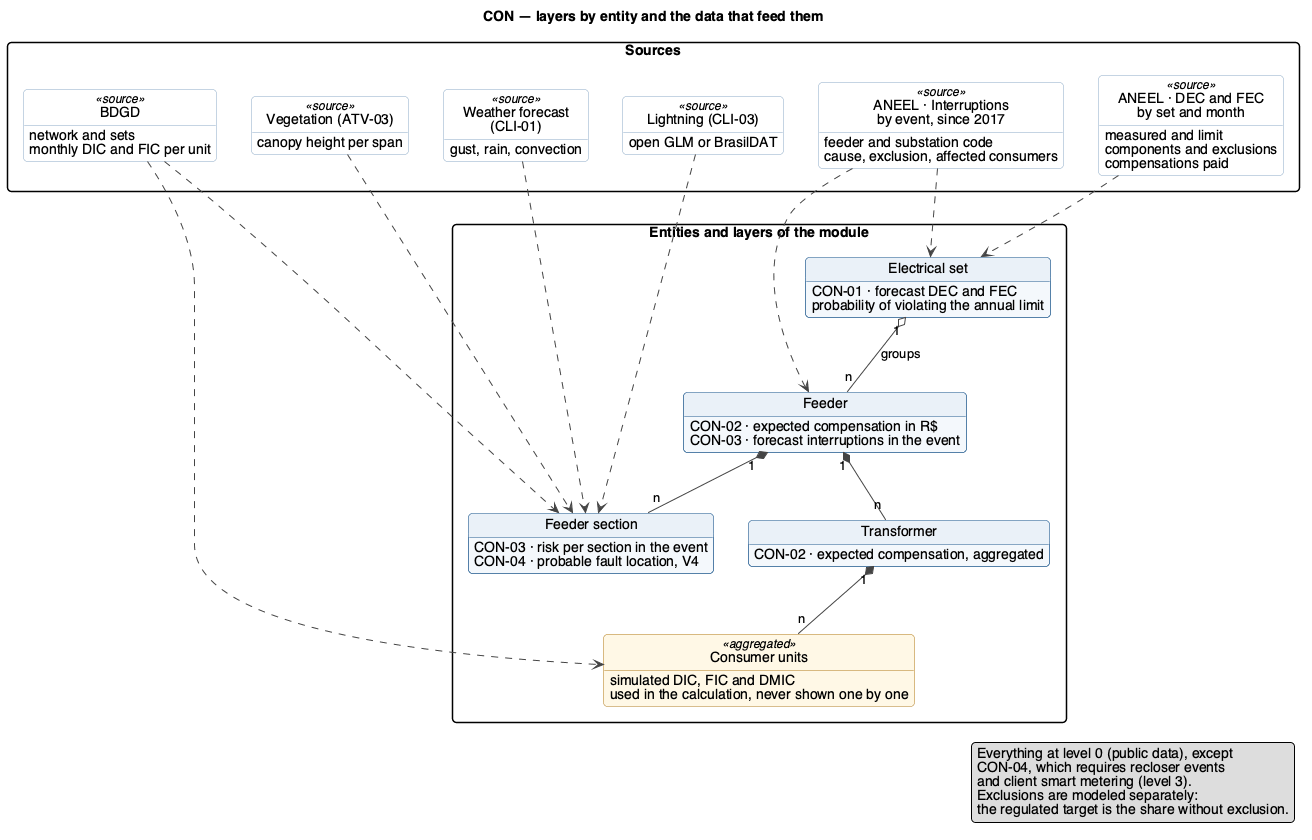
\includegraphics[width=\textwidth]{con-camadas-en.png}
\caption{CON: layers by entity and the data that feed them. Level 0, except
CON-04; CON-02 requires level 1 for the current quarter.}
\end{figure}

\begin{figure}[H]
\centering
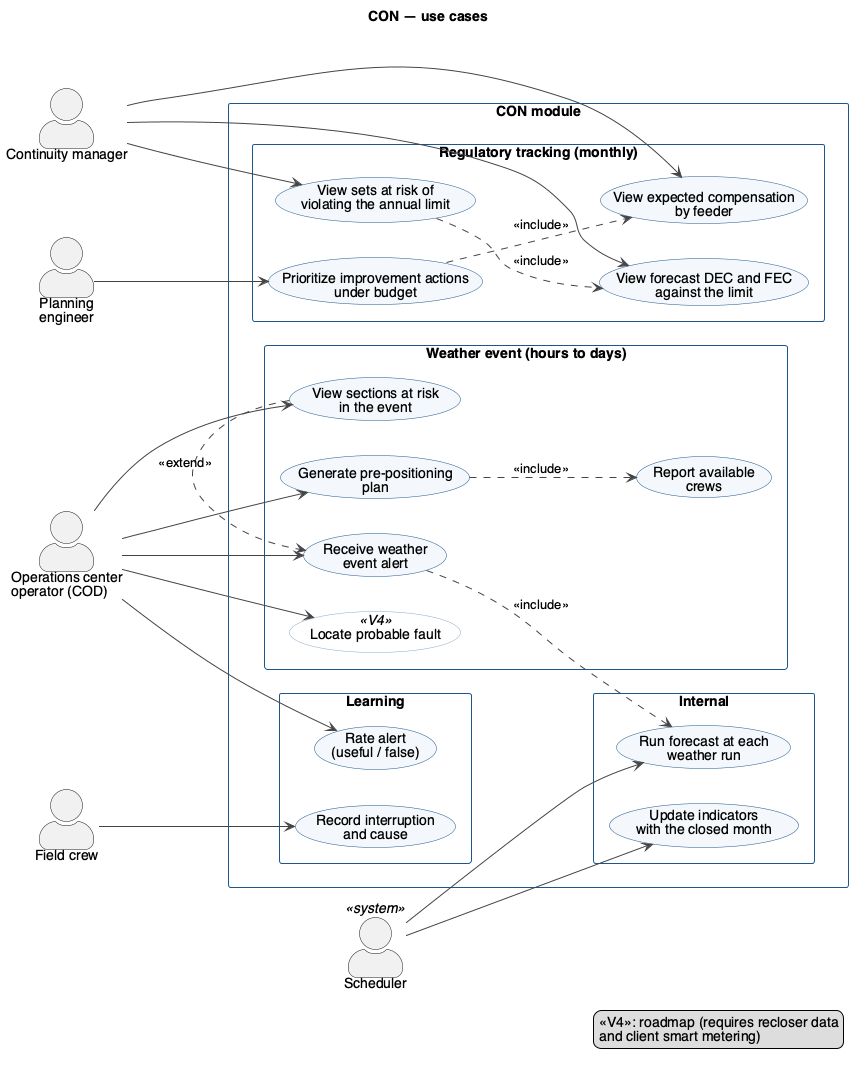
\includegraphics[width=0.78\textwidth]{con-casos-de-uso-en.png}
\caption{CON: use cases, separated by the module's two rhythms.}
\end{figure}

\begin{figure}[H]
\centering
\begin{minipage}[t]{0.40\textwidth}\centering
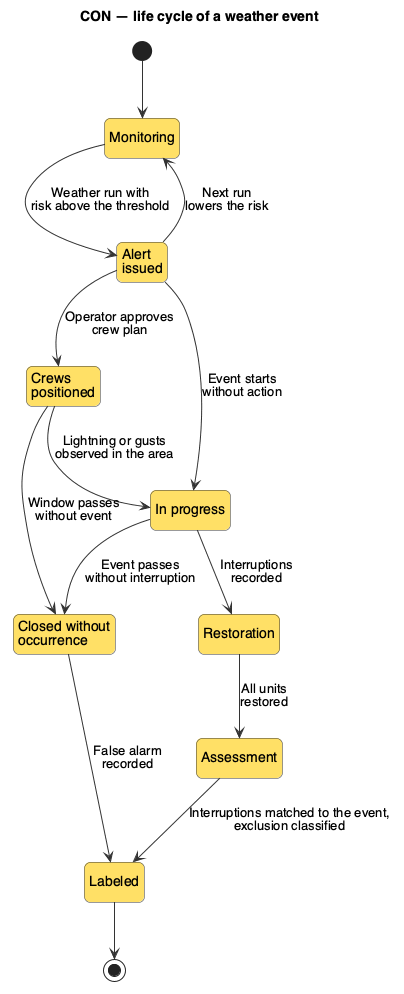
\includegraphics[width=\linewidth]{con-estados-evento-en.png}
\end{minipage}\hfill
\begin{minipage}[t]{0.56\textwidth}\centering
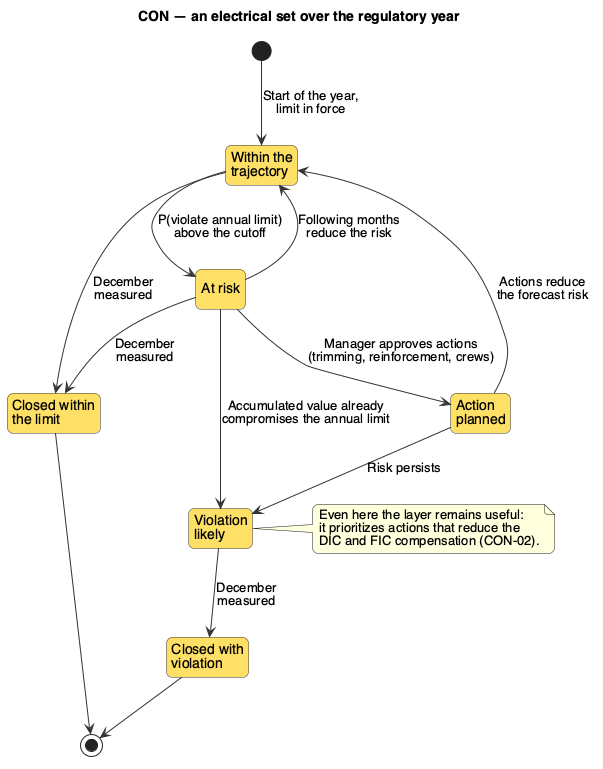
\includegraphics[width=\linewidth]{con-estados-conjunto-en.png}
\end{minipage}
\caption{CON: state machines of the weather event (left) and of the electrical
set in the regulatory year (right). Labeled events, including false
alarms, return as training labels.}
\end{figure}

\begin{figure}[H]
\centering
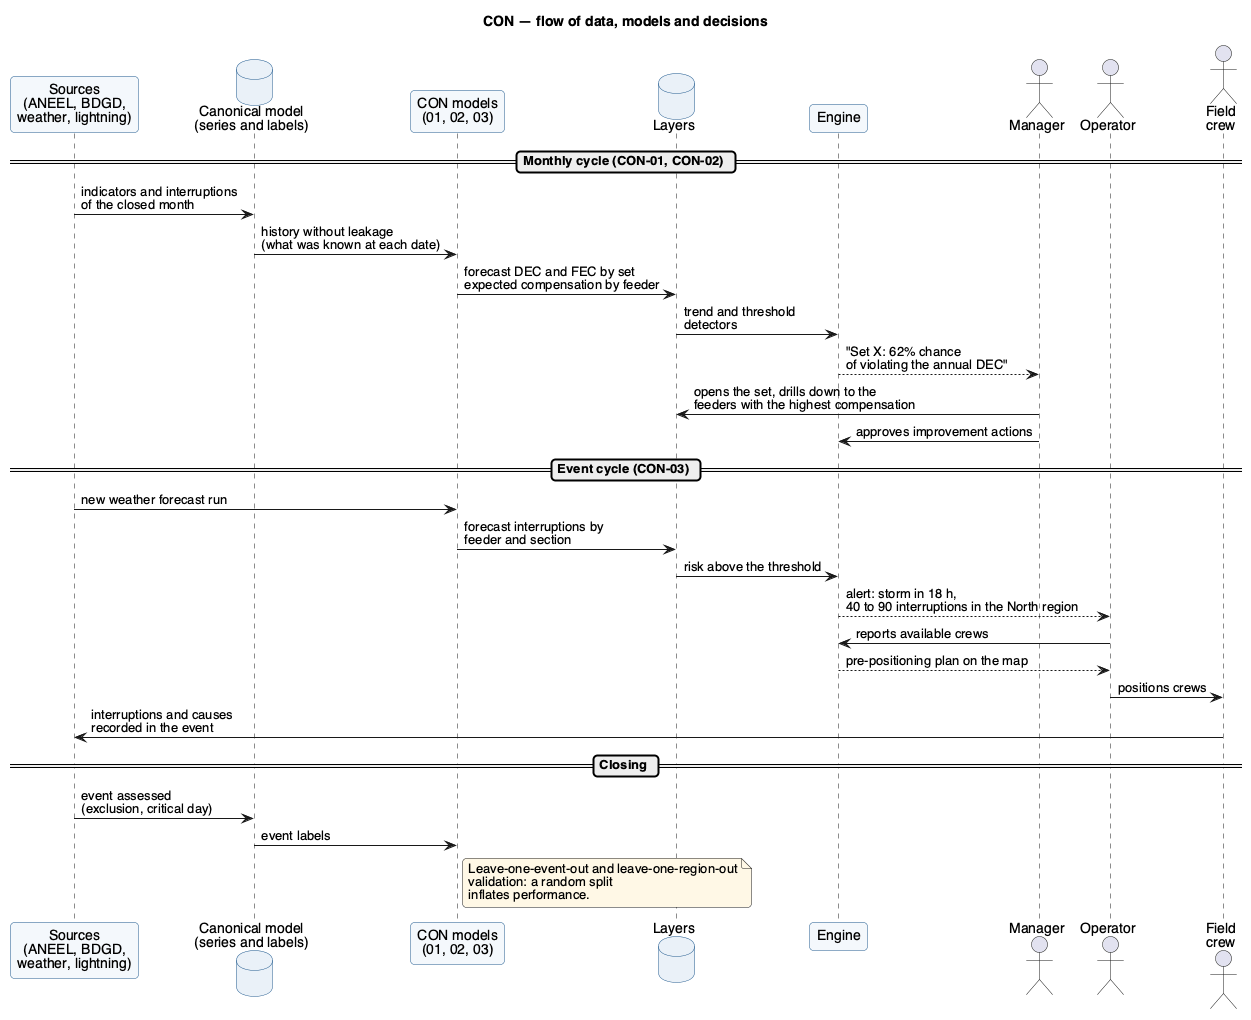
\includegraphics[width=\textwidth]{con-fluxo-en.png}
\caption{CON: flow of the monthly cycle, the event cycle and the closing, with
leave-one-event-out and leave-one-region-out validation.}
\end{figure}

\subsection*{References for this section}
{\small
\begin{enumerate}[label={[\arabic*]},leftmargin=2.2em,itemsep=1pt]
\item ANEEL, Indicadores Coletivos de Continuidade: \url{https://dadosabertos.aneel.gov.br/dataset/indicadores-coletivos-de-continuidade-dec-e-fec}
\item ANEEL, Interrupções nas Redes de Distribuição: \url{https://dadosabertos.aneel.gov.br/dataset/interrupcoes-de-energia-eletrica-nas-redes-de-distribuicao}
\item ANEEL, Ocorrências Emergenciais: \url{https://dadosabertos.aneel.gov.br/dataset/ocorrencias-emergenciais-nas-redes-de-distribuicao}
\item ANEEL, PRODIST Module 8 (REN 956/2021): \url{https://www.gov.br/aneel/pt-br/centrais-de-conteudos/procedimentos-regulatorios/prodist}
\item REN ANEEL 956/2021, PRODIST Module 1 (Critical Day)
\item ANEEL, BDGD: \url{https://dadosabertos.aneel.gov.br/dataset/base-de-dados-geografica-da-distribuidora-bdgd}
\item Radatz, bdgd2opendss: \url{https://github.com/PauloRadatz/bdgd2opendss}
\item Aderaldo (2023), BDGD-Tools, UFC: \url{https://repositorio.ufc.br/handle/riufc/75567}
\item[] \refstepcounter{enumi}
\item ONS, constrained-off by plant: \url{https://dados.ons.org.br/dataset/restricao_coff_eolica_detail}
\item ONS, RO-AO.BR.13, constrained-off measurement
\item ONS Dados Abertos, lines and availability: \url{https://dados.ons.org.br/dataset/linha-transmissao}
\item EPE, transmission databases: \url{https://www.epe.gov.br/pt/leiloes-de-energia/leiloes-de-transmissao/bases-de-dados}
\item ANEEL, REN 729/2016 (Parcela Variável)
\item ANEEL, Plano de Desenvolvimento da Distribuição: \url{https://www.gov.br/aneel/pt-br/assuntos/distribuicao/plano-de-desenvolvimento-da-distribuicao}
\item INPE/ELAT, RINDAT and BrasilDAT: \url{http://www.inpe.br/webelat/rindat/}
\item NASA Earthdata, GLM: \url{https://www.earthdata.nasa.gov/data/instruments/glm}
\item INMET, BDMEP: \url{https://bdmep.inmet.gov.br/}
\item Wanik et al.\ (2015), \emph{Natural Hazards} 79, doi:10.1007/s11069-015-1908-2
\item Cerrai et al.\ (2019), \emph{IEEE Access} 7
\item UConn Outage Prediction Model, AGU (2021)
\item Extratropical storms outages, \emph{NHESS} 21 (2021)
\item Essus, Vatsavai and Rachunok (2026), leakage in interruption models: \url{https://arxiv.org/abs/2608.24665}
\item Stanishevska and Guikema (2025): \url{https://arxiv.org/abs/2510.03959}
\item GNN and tree risk from LiDAR, \emph{RESS} (2025)
\item Lin et al.\ (2023), PowerFlowNet: \url{https://arxiv.org/abs/2311.03415}
\item Ghamizi et al.\ (2024), PowerFlowMultiNet: \url{https://arxiv.org/abs/2403.00892}
\item Okoyomon, Yaniv and Goebel (2025): \url{https://arxiv.org/abs/2509.25158}
\item PF$\Delta$ (2025): \url{https://arxiv.org/abs/2510.22048}
\item SafePowerGraph (2024): \url{https://arxiv.org/abs/2407.12421}
\item Nakiganda and Chatzivasileiadis, GNN for contingencies: \url{https://arxiv.org/abs/2310.04213}
\item N-k with input-convex networks (2024): \url{https://arxiv.org/abs/2410.00796}
\item Baran and Wu (1989), \emph{IEEE Trans.\ Power Delivery} 4(2)
\item Jacob et al.\ (2024), \emph{Nature Communications}
\item PI-GNN for reconfiguration (2023): \url{https://arxiv.org/abs/2310.00728}
\item Karabulut, Manna and Develder (2026): \url{https://arxiv.org/abs/2604.20403}
\item Fault location in LV with a digital twin, \emph{Energies} 16 (2023), doi:10.3390/en16237850
\item Overload alarm in distribution transformers (2024)
\item Investment in distribution networks with correlation between projects, \emph{Frontiers in Energy Research} (2021)
\item Interruption limits in Brazil with AI, \emph{Energies} 16 (2023), doi:10.3390/en16197012
\item Prediction of quality indicators with neural networks, SBSE
\item IEEE C57.91, loading guide
\end{enumerate}}

% Research cards: ATV, GER
% Checked on the web on September 23, 2026. "(to be confirmed)" marks what was not verified in a source.

\section{Assets and renewable generation}

\subsection*{Shared sources}
\begin{itemize}
  \item \textbf{ONS Dados Abertos} (CC-BY, also mirrored on AWS) [8]: generation
    by plant on an hourly basis [5], hourly capacity factor of wind and
    solar plants [6], half-hourly constrained-off by plant since 2021 [1--4],
    availability of lines and transformers [7]. ONS warns that the data
    are revised after publication.
  \item \textbf{ANEEL}: SIGA (plant registry by CEG) [9], SIGEL (plants and
    lines in shapefile, wind turbines in SIGEL-EOL) [10], BDGD [11],
    interruptions in the distribution networks [12].
  \item \textbf{Join key}: the constrained-off data carry \texttt{ceg} and
    \texttt{id\_ons} [4], which links ONS, SIGA and SIGEL through the CEG; plant
    groups appear without a CEG and require a dedicated correspondence table.
\end{itemize}

% ---------------------------------------------------------------------------
\subsection{ATV \textperiodcentered{} Assets and maintenance}

\begin{ficha}{ATV-01 \textperiodcentered{} Power transformer health index}{V3}
\campo{Data} From the client: dissolved gas chromatography (H$_2$, CH$_4$,
C$_2$H$_6$, C$_2$H$_4$, C$_2$H$_2$, CO, CO$_2$), oil physicochemical tests,
furans, loading, age, work order history. Standards: IEC
60599:2022 [28]; IEEE C57.104-2019, which replaced total gas thresholds with
percentiles by gas, deltas between samples and annual rates [27]; Duval
triangles and pentagons [30]; CIGRE TB 761 assessment indices [31]. Public
reference data: IEC TC10, with 117 labeled samples [29].
\campo{Approaches} Baseline: standard-based rules combined into a
CIGRE-style weighted index. Recommended: gradient boosting that uses the standards
as variables (ratios, Duval coordinates, deltas, rates, loss of life
by IEEE C57.91 [33]), with the later event (failure or
intervention) as the label and not the Duval class; with calibration and SHAP. Recent review:
Zahra et al.\ (2025) [32].
\campo{Metrics} F1 by fault class (diagnosis); AUC-PR for failure or
intervention within 12 months and hit rate at the top of the list (prognosis); agreement
with an expert.
\campo{Pitfalls} Validation on IEC TC10 alone (117 samples) does not support
generalization;
rates require three or more samples, rare in practice; a change of laboratory and
oil treatment create artificial jumps.
\end{ficha}

\begin{ficha}{ATV-02 \textperiodcentered{} Failure risk by equipment}{V3}
\campo{Data} Public: BDGD (segments, transformers, switches, installation
date) [11] and interruptions by event [12]; ONS for the basic grid [7].
From the client: registry with replacements, structured work orders (ATV-05).
\campo{Approaches} Baseline: Weibull by class and Cox. Recommended:
random survival forest or boosting with a survival loss and
time-varying covariates (weather, loading), handling censoring and left
truncation [34,35]. Recent literature: DeepSurv and discrete-time
neural models [36]. At the feeder level: failure count per km and year.
\campo{Metrics} C-index (including time-dependent), Integrated Brier
Score, calibration at 12 months, hit rate at the top of the list.
\campo{Pitfalls} Left truncation (survivor bias); replacements without
a record; external causes mixed with wear (competing risks).
\end{ficha}

\begin{ficha}{ATV-03 \textperiodcentered{} Vegetation near the network}{V3}
\campo{Data} Network geometry (BDGD [11], SIGEL [10]). Public canopy
height: global 10~m map for 2020 (Lang et al.\ 2023) [37] and 1~m map
(Meta and WRI, Tolan et al.\ 2024, images from 2017 to 2020) [38]. Sentinel-2
for updating. Client LiDAR when available.
\campo{Approaches} Baseline: canopy height and NDVI intersected with a
buffer of the span. Recommended: dense vegetation segmentation and height
regression with Sentinel-2 and GEDI; Brazilian case (SENAI and Cemig, 2025/2026) with
RMSE of 7.7~m and MAE of 5~m against LiDAR [39]. With LiDAR: direct distance
between conductor and vegetation. Recent literature: SAM adapted for transmission
corridors [40].
\campo{Metrics} IoU and F1 of the segmentation; height error against LiDAR; recall
of critical spans in the field; correlation with vegetation interruptions [12].
\campo{Pitfalls} An error of 5 to 8~m is of the order of the safety clearance zone: it serves
to prioritize, not to measure distance. Static maps age with
growth and tree trimming.
\end{ficha}

\begin{ficha}{ATV-04 \textperiodcentered{} Defects in inspection images}{V4}
\campo{Data} Client drone images. Public: CPLID (synthetic
defects) [21]; InsPLAD, with 10,607 images, 17 asset classes and 6 defect
types, but only 402 defect samples [22]; TTPLA (towers and cables) [23];
UPID [24].
\campo{Approaches} Baseline: YOLO fine-tuned for components [26].
Recommended: two stages, detect the component and classify the defect or
detect an anomaly in the crop [22]. Recent literature: RT-DETR (CVPR 2024) [25];
SAM for pre-annotation with a human in the loop.
\campo{Metrics} mAP by class; recall by critical defect; precision by
structure (what becomes a work order).
\campo{Pitfalls} Rare defects; models trained on synthetic defects
may not generalize; Brazilian
insulator types differ; each image has to be associated with the BDGD
structure.
\end{ficha}

\begin{ficha}{ATV-05 \textperiodcentered{} Structuring of work orders and causes}{V3}
\campo{Data} Free text of the client's work orders; causes from the interruptions
dataset as a weak label [12]. Schemas: MaintIE (224 entities, 6
relations) [41] and ISO 14224 for failure modes [42].
\campo{Approaches} In failure mode classification into 22 ISO 14224 codes,
a fine-tuned GPT-3.5 reached F1 0.80, against 0.60 for a text
classifier and 0.46 for the model without fine-tuning [42]. Recommended: language model with
JSON output constrained to a schema (component, failure mode, cause, action),
client examples, light fine-tuning and human review by sampling.
\campo{Metrics} F1 by field; valid JSON rate; C-index gain in ATV-02
with the extracted variables.
\campo{Pitfalls} The benchmarks are in English and the work order text is short,
abbreviated and regional; each extracted field has to keep the excerpt that
justifies it; LGPD.
\end{ficha}

\begin{ficha}{ATV-06 \textperiodcentered{} Remaining useful life and maintenance plan}{V4}
\campo{Data} ATV-01 and ATV-02; client costs, crews and budget;
consequence of failure by the affected customers (BDGD, interruptions).
\campo{Approaches} Baseline: risk × criticality matrix. Recommended:
monetized risk by asset and integer optimization under crews and regions (to
be confirmed as the standard). Recent literature: stochastic optimization under the
uncertainty of the survival curve.
\campo{Pitfalls} Few end-of-life cases to validate; the optimization amplifies
calibration errors.
\end{ficha}

% ---------------------------------------------------------------------------
\subsection{GER \textperiodcentered{} Renewable generation}

\begin{ficha}{GER-01 \textperiodcentered{} Forecast generation by plant (P10--P90)}{V2}
\campo{Data} Location and specifications: SIGA and SIGEL [9,10]. \textbf{Public observed
generation}: ONS by plant, hourly [5], and half-hourly verified
generation in the constrained-off data [4]; covers Type I, II-B and II-C plants (II-C
aggregated into groups). Weather forecast: ECMWF opened its whole real-time
catalog under CC-BY in October 2025 [53]. Client SCADA in 10-minute
averages.
\campo{Approaches} Baseline: persistence, climatology, power
curve applied to the forecast. Recommended: quantile gradient boosting on
numerical weather prediction variables, the winning method of GEFCom2014 [52], with
conformal recalibration. Onboarding without history: foundation models with the
weather forecast as a future covariate (Chronos-2 [46], TimesFM 2.5 [47],
Moirai 2.0 [48]); synthetic histories generated by a physical model reduced the
error by 1.7 to 2 times at 440 photovoltaic plants [50]. In [49], no
approach had the lowest error in all cases. In Brazil, ERA5 outperformed MERRA-2 for wind [54].
\campo{Metrics} nMAE and nRMSE by capacity; pinball and CRPS; P10--P90
coverage; skill against persistence; by horizon and without curtailment.
\campo{Pitfalls} \textbf{Train on the reference generation, not on the
delivered generation}, so as not to learn the curtailment [4]; ONS revisions; leakage
through observed weather; UTC versus local time.
\end{ficha}

\begin{ficha}{GER-02 \textperiodcentered{} Ramp alerts}{V2}
\campo{Approaches} There is no standard definition: a ramp is magnitude, duration
(typically 1 to 4~h), time and direction, with a threshold by plant size [55].
Baseline: variation threshold on the P50. Recommended: ramp
probability computed on \textbf{time-coherent scenarios}, not on marginal
quantiles, which create spurious ramps.
\campo{Metrics} POD, FAR and CSI with a phase tolerance of one hour; Brier;
lead time; alerts per week.
\end{ficha}

\begin{ficha}{GER-03 \textperiodcentered{} Satellite nowcasting (0 to 6 h)}{V3}
\campo{Data} GOES-19, operational GOES-East since April 4, 2025, on AWS without
an account [13,14]; ABI with visible at 0.5~km and full disk every 10 minutes [15];
surface irradiance (DSR) at 2~km and 10 minutes in the Enterprise algorithm
[16]; daily radiation from INPE [17].
\campo{Approaches} Baseline: persistence of the clear-sky index and
cloud motion vectors. Recommended: U-Net on cloud index
sequences, converted into power by plant [57,60]; Brazilian case with
GOES-16 in Petrolina [59]. Recent literature, probabilistic: SHADECast, which
extends the useful horizon by about 26 minutes [56]. Beyond 2 to 3~h,
combine with numerical weather prediction [53].
\campo{Metrics} RMSE of irradiance and power; skill against persistence
by lead time; CRPS.
\campo{Pitfalls} Parallax and resolution against small plants; latency;
discontinuity in the switch from GOES-16 to GOES-19.
\end{ficha}

\begin{ficha}{GER-04 \textperiodcentered{} Curtailment detected and flagged}{V2}
\campo{Data} ONS constrained-off, dictionary v1.5 (September 2026): generation,
limited generation, availability, reference, final reference (only for
REL, sent to CCEE), reason (REL, CNF, ENE, PAR), origin (LOC, SIS), unrealized
energy and minutes by reason [4]. Report of the ONS GT Curtailment
[62]. SCADA with setpoints.
\campo{Approaches} Baseline: rules on the limited generation and the
constraint minutes; in SCADA, setpoint below rated power. Recommended:
\textbf{available power} model (normal behavior, GER-05);
curtailment is available minus delivered when there is a limit, which detects
unreported cuts and contests the ONS reference; power curve
cleaning by anomaly detection [64].
\campo{Pitfalls} The 30-minute resolution hides short cuts; reimbursement
rules change by resolution (to be confirmed).
\end{ficha}

\begin{ficha}{GER-05 \textperiodcentered{} Actual × expected performance}{V3}
\campo{Data} SCADA, resource, curtailment from GER-04. Public, for
development: Kelmarsh and Penmanshiel (10-minute SCADA, CC-BY) [18,19];
PVDAQ from NREL [68].
\campo{Approaches} Baseline: power curve by bins and
performance ratio. Recommended: normal behavior model (boosting or
GAM) trained on a healthy period; for photovoltaic, fitted pvlib.
Tools: OpenOA (NREL) [65] and RdTools for degradation [71].
\campo{Pitfalls} Training the expected value on data that already contain the loss; the
cleaning may retain only about 31\% of the data [64].
\end{ficha}

\begin{ficha}{GER-06 \textperiodcentered{} Turbine health}{V3}
\campo{Data} SCADA with bearing, generator and gearbox
temperatures. Labeled: CARE to Compare (Fraunhofer, 2024), 95 datasets, 36
turbines, 44 labeled events, with the CARE metric (coverage, accuracy,
reliability, earliness) [20].
\campo{Approaches} Review: Tautz-Weinert and Watson (2017) [66]. Chesterman et
al.\ (2023), at 5 plants: Elastic Net competitive with LightGBM and neural networks;
normalize by the fleet median; exclude the 4 months before the failure from training;
no family dominates [67]. Recommended: normal behavior with
fleet normalization and alarm with persistence.
\campo{Metrics} CARE score; days of lead time; false alarms per turbine
per year.
\campo{Pitfalls} Few failures; pre-failure data contaminate the normal; climate
of the Northeast different from that of the European datasets.
\end{ficha}

\begin{ficha}{GER-07 \textperiodcentered{} Soiling and solar cleaning schedule}{V4}
\campo{Approaches} Kimber (linear accumulation until rain above a threshold) and HSU
(by particulate mass), both in pvlib [69,70]; from production, SRR
(Deceglie et al.\ 2018) in RdTools [71]; report IEA PVPS T13-21:2022 [72].
Thresholds of rain that cleans range from 0.3 to 20~mm/day [73]. Decision: clean
when the expected loss until the next forecast rain exceeds the cost.
\campo{Pitfalls} Confusing soiling with degradation or shading;
unrecorded cleanings break the SRR.
\end{ficha}

\begin{ficha}{GER-08 \textperiodcentered{} Forecast aggregate generation by submarket}{cond}
\campo{Approaches} Sum of the forecasts by plant with upscaling for those without
a forecast; hierarchical reconciliation (plant, state, submarket) [74] and a
value-oriented version [75]. Aggregate quantiles require joint scenarios: the sum of
quantiles is not the quantile of the sum.
\campo{Pitfalls} Entry of new plants (update through SIGA); stating whether the
forecast is of available or delivered power; invisible DG.
\end{ficha}

\subsection*{References for this section}
{\small
\begin{enumerate}[label={[\arabic*]},leftmargin=2.2em,itemsep=1pt]
\item ONS, wind constrained-off: \url{https://dados.ons.org.br/dataset/restricao_coff_eolica_usi}
\item ONS, wind constrained-off by plant: \url{https://dados.ons.org.br/dataset/restricao_coff_eolica_detail}
\item ONS, photovoltaic constrained-off: \url{https://dados.ons.org.br/dataset/restricao_coff_fotovoltaica_detail}
\item ONS, constrained-off dictionary v1.5 (September 2026)
\item ONS, hourly generation by plant: \url{https://dados.ons.org.br/dataset/geracao-usina-2}
\item ONS, capacity factor: \url{https://dados.ons.org.br/dataset/fator-capacidade-2}
\item ONS, transmission function availability: \url{https://dados.ons.org.br/dataset/ind_disponibilidade_ft_trlt}
\item ONS on AWS: \url{https://registry.opendata.aws/ons-opendata-portal/}
\item ANEEL, SIGA: \url{https://dadosabertos.aneel.gov.br/dataset/siga-sistema-de-informacoes-de-geracao-da-aneel}
\item ANEEL, SIGEL: \url{https://sigel.aneel.gov.br/portal/home/}
\item ANEEL, BDGD: \url{https://dadosabertos.aneel.gov.br/dataset/base-de-dados-geografica-da-distribuidora-bdgd}
\item ANEEL, interruptions: \url{https://dadosabertos.aneel.gov.br/dataset/interrupcoes-de-energia-eletrica-nas-redes-de-distribuicao}
\item NOAA GOES on AWS: \url{https://registry.opendata.aws/noaa-goes/}
\item NOAA, GOES-19 on NODD
\item GOES-R ABI: \url{https://www.goes-r.gov/spacesegment/abi.html}
\item NCEI, ABI L2 DSR
\item INPE, daily mean solar radiation (GOES-16)
\item Kelmarsh: \url{https://zenodo.org/records/5841834}
\item Penmanshiel: \url{https://zenodo.org/records/5946808}
\item Gück, Roelofs and Faulstich (2024), CARE to Compare: \url{https://arxiv.org/abs/2404.10320}
\item CPLID: \url{https://github.com/InsulatorData/InsulatorDataSet}
\item Vieira e Silva et al.\ (2023), InsPLAD, \emph{IJRS} 44(23): \url{https://arxiv.org/abs/2311.01619}
\item Abdelfattah et al.\ (2020), TTPLA: \url{https://arxiv.org/abs/2010.10032}
\item UPID: \url{https://github.com/heitorcfelix/public-insulator-datasets}
\item Zhao et al.\ (2024), RT-DETR, CVPR: \url{https://arxiv.org/abs/2304.08069}
\item MAP-YOLOv8, \emph{Scientific Reports} (2025)
\item IEEE C57.104-2019
\item IEC 60599:2022
\item IEC TC10 in \emph{IET GTD} (2021); IEEE DataPort DGA dataset
\item Duval, triangles and pentagons
\item CIGRE TB 761 (2019)
\item Zahra et al.\ (2025): \url{https://arxiv.org/abs/2504.15310}
\item IEEE C57.91, loading guide
\item Survival models in power networks, \emph{Sensors} (2026), doi:10.3390/s26061915
\item Ishwaran et al.\ (2008), Random Survival Forests, \emph{Ann.\ Appl.\ Stat.}
\item Katzman et al., DeepSurv: \url{https://arxiv.org/abs/1606.00931}
\item Lang et al.\ (2023), \emph{Nature Ecology \& Evolution} 7:1778--1789
\item Tolan et al.\ (2024), \emph{RSE} 300:113888: \url{https://registry.opendata.aws/dataforgood-fb-forests/}
\item HVAS (SENAI and Cemig), ISPRS Annals X-3-W4-2025
\item SAM for transmission corridors: \url{https://arxiv.org/abs/2505.22105}
\item Bikaun et al.\ (2024), MaintIE, LREC-COLING
\item Stewart et al., LLMs for failure modes: \url{https://arxiv.org/abs/2309.08181}
\item LLM benchmark on turbine logs: \url{https://arxiv.org/abs/2509.06813}
\item KPI extraction from work orders: \url{https://arxiv.org/abs/2311.04064}
\item Brundage et al., Technical Language Processing, \emph{Manufacturing Letters} 27
\item Ansari et al., Chronos-2: \url{https://arxiv.org/abs/2510.15821}
\item TimesFM 2.5: \url{https://huggingface.co/google/timesfm-2.5-200m-pytorch}
\item Moirai 2.0: \url{https://arxiv.org/abs/2511.11698}
\item Za'ter and Hodge (2026): \url{https://arxiv.org/abs/2604.22077}
\item Longarini et al.\ (2026), synthetic histories: \url{https://arxiv.org/abs/2606.07457}
\item Chronos, TimesFM and Moirai, original versions
\item Hong et al.\ (2016), GEFCom2014, \emph{IJF}; Landry et al., GBM
\item ECMWF, open real-time catalog (2025)
\item Gruber et al., reanalyses in Brazil: \url{https://arxiv.org/abs/1904.13083}
\item Gallego-Castillo et al.\ (2015), ramps, \emph{RSER} 52
\item Carpentieri et al., SHADECast: \url{https://arxiv.org/abs/2312.11966}
\item Straub et al.\ (2024), \emph{Solar RRL}
\item SunCast: \url{https://arxiv.org/abs/2201.06173}
\item GHI and DNI with GOES-16 in Petrolina, \emph{Int.\ J.\ Energy Environ.\ Eng.}
\item Satellite nowcasting with deep learning, \emph{Solar Energy} (2024)
\item Shi et al., ConvLSTM: \url{https://arxiv.org/abs/1506.04214}
\item ONS, RT DGL-ONS 0189-2025, GT Curtailment
\item Canal Solar, cuts in 2026 (secondary source)
\item Power curve cleaning in SCADA, \emph{Renewable Energy} (2022)
\item NREL OpenOA: \url{https://github.com/NREL/OpenOA}
\item Tautz-Weinert and Watson (2017), \emph{IET RPG} 11, doi:10.1049/iet-rpg.2016.0248
\item Chesterman et al.\ (2023), \emph{Wind Energy Science} 8:893
\item NREL PVDAQ: \url{https://data.openei.org/submissions/4568}
\item Kimber soiling model in pvlib
\item HSU soiling model
\item RdTools SRR; Deceglie et al.\ (2018), \emph{IEEE JPV} 8(2)
\item IEA PVPS T13-21:2022, soiling losses
\item Cleaning by rain, \emph{Solar RRL} (2024)
\item Hansen et al.\ (2023), spatial reconciliation of wind forecasts, \emph{Wind Energy}
\item Value-oriented reconciliation: \url{https://arxiv.org/abs/2501.16086}
\end{enumerate}}

% Research cards: MER, CLI, DRE, ENG
% Checked on the web on September 23, 2026. "(to be confirmed)" marks what was not verified in a source.

\section{Market, weather, demand response and engine}

% ---------------------------------------------------------------------------
\subsection{MER \textperiodcentered{} Market and price}

\begin{nota}
\textbf{Conditional track.} The three features in this module, with CAR-08 and
GER-08, are outside the phased roadmap: they enter only if the target client
question is settled in favor of generator and energy trader. The research
is recorded so that the decision, when it comes, does not start from zero.
\end{nota}

\begin{nota}
\textbf{Access to CCEE data.} The CCEE Dados Abertos portal has a security
block (application firewall) that stops clients outside the access policy
and directs them to open a ticket with the error code and the IP [1,2]. The
CCEE publishes tutorials on automation by API, and the download from a CKAN
endpoint (\texttt{/datastore/dump/<id>}) worked without a block on September 23, 2026.
Automated collection was possible with few requests, an identifiable
user-agent, a local cache and download of the yearly CSVs instead of scraping.
\end{nota}

\begin{ficha}{MER-01 \textperiodcentered{} Forecast PLD by submarket (quantiles)}{cond}
\campo{Data} \emph{PLD\_HORARIO} from the CCEE: one CSV per year, hourly from 2021 to
2026 and weekly from 2001 to 2020, CC-BY 4.0 license, daily update [3].
Regulatory limits for 2026: floor R\$~57.31/MWh, structural cap
R\$~785.27/MWh and hourly cap R\$~1,611.04/MWh (Despacho ANEEL 3.850/2025)
[5]. NEWAVE/DECOMP/DESSEM decks in the Acervo CCEE, including shadow decks [6];
DESSEM decks also at the ONS [7]. ONS Dados Abertos: half-hourly load,
generation by plant and half-hourly CMO [8].
\campo{Approaches} Baseline: seasonal naive and LEAR (autoregressive
with LASSO), used as a reference and implemented in \emph{epftoolbox} [10].
Recommended: gradient boosting with quantile loss on CMO, forecast load and
renewables, reservoir storage and the deck in force, with
conformal calibration (to be confirmed). Recent literature: emulation of DESSEM by
a surrogate model and networks that forecast parametric distributions [10].
\campo{Metrics} Pinball and CRPS, coverage and width of the intervals, MAE
relative to the naive, Diebold--Mariano test.
\campo{Pitfalls} Structural break on January 1, 2021 (the PLD became hourly,
computed by DESSEM) [4]; new future cost function on October 12, 2025 [6];
distribution censored at the floor and at the cap; ONS series revised after
publication, which requires storing what was known at each date [8]. The
Projeto Meta II proposes bid-based pricing and two PLDs (ex-ante and ex-post), with
rollout planned for June 2028 [9], which will break the series if rolled out.
\end{ficha}

\begin{ficha}{MER-02 \textperiodcentered{} Joint scenarios of generation, load and price}{cond}
\campo{Data} Probabilistic outputs of GER-01, CAR-08 and MER-01; joint
history from the ONS and the CCEE [3,8].
\campo{Approaches} Baseline: independent scenarios or bootstrap of
historical blocks. Recommended: Gaussian copula on the predictive
marginals (Pinson et al.\ 2009) [11]; alternative with the order of the members of the
weather ensemble (ECC and dual-ECC) [12]. Recent literature: vine copulas and
deep generators (to be confirmed).
\campo{Metrics} Energy score and variogram score, multivariate rank
histograms, CRPS by marginal (\emph{scoringrules} library) [13].
\campo{Pitfalls} The dependence changes with the hydrological regime, and a
stationary copula underestimates extreme joint events (drought with peak load).
\end{ficha}

\begin{ficha}{MER-03 \textperiodcentered{} Bid optimization and battery dispatch}{cond}
\campo{Data} Scenarios from MER-02, hourly PLD and technical parameters of the
battery. Context: Portaria MME 136/2026 defines the first capacity reserve
auction for batteries (December 2026, 15-year contracts starting
in August 2028), with availability revenue and not free arbitrage
[14].
\campo{Approaches} Baseline: deterministic optimization on the point
forecast. Recommended: two-stage stochastic programming or CVaR,
on a rolling window. Recent literature: decision-focused learning; minimizing the
CRPS does not guarantee the best bid [15].
\campo{Metrics} Revenue against the optimum with perfect information (regret),
CVaR of revenue, degradation cost.
\campo{Pitfalls} Today the PLD comes from a cost model, not from bids; ``bid''
only makes sense with the hybrid model (2028 onward) [9]. Simplified
degradation overestimates revenue. Low map fit.
\end{ficha}

% ---------------------------------------------------------------------------
\subsection{CLI \textperiodcentered{} Weather context}

\begin{ficha}{CLI-01 \textperiodcentered{} Forecast weather}{V2}
\campo{Data} ECMWF Open Data: IFS and AIFS (deterministic and ensemble), 0.25°
grid, four runs per day, CC-BY 4.0 license with commercial use
allowed and attribution required; the portal keeps only the runs of the
last 2 to 3 days, with cloud mirrors [16,17]. NOAA GFS 0.25° on AWS,
open, with long history at NCAR [18]. CPTEC/INPE: BAM, WRF, Eta and BRAMS,
with citation required [19]. INMET: hourly automatic stations (portal with
90 days) and BDMEP for the history, with a lag of 1 to 3 months [20].
\campo{Approaches} Baseline: raw forecast interpolated to the
entities. Recommended: statistical post-processing by entity (MOS,
EMOS, quantile regression) with downscaling. Recent literature: global ML
models (AIFS, GraphCast-GFS) [16,18]. Tools: \emph{herbie},
\emph{xarray}/\emph{cfgrib}, \emph{xskillscore} [17].
\campo{Metrics} RMSE and MAE by variable and horizon, CRPS of the ensemble,
reliability diagram, skill against climatology and persistence.
\campo{Pitfalls} \textbf{Archive every run from the first day}: without
that, there is no history of forecasts to train without leakage. Changes of
model version break the post-processing. The ECMWF attribution has to
appear on the map.
\end{ficha}

\begin{ficha}{CLI-02 \textperiodcentered{} Observed satellite and radar}{V2}
\campo{Data} GOES-East has been \textbf{GOES-19} since April 2025 (75.2°W),
with ABI and GLM on AWS Open Data in NetCDF4; there were outages (ABI restored
in July 2026) [21]. REDEMET/DECEA radar by API with a key, but as a PNG
image, useful to display and not to model [22]. CEMADEN: rain gauges and
dual-polarization radars, with volumetric data on request (to be confirmed)
[23].
\campo{Approaches} Baseline: display mosaics. Recommended: precipitation
nowcasting from 0 to 6 h with \emph{pysteps} (optical flow and stochastic
ensembles) [24]. Recent literature: deep nowcasting (ConvGRU, diffusion).
\campo{Metrics} CSI, POD and FAR by threshold; FSS; CRPS [24].
\campo{Pitfalls} Uneven radar coverage across the territory; gaps and
latency of GOES.
\end{ficha}

\begin{ficha}{CLI-03 \textperiodcentered{} Lightning and severe events}{V3}
\campo{Data} BrasilDAT (ELAT/INPE): detects cloud-to-ground and
intracloud strokes; access by contacting ELAT, \textbf{it is not open} [25].
Open alternative: GLM on GOES-19, optical detection of total lightning with
uniform efficiency over Brazil [21,26].
\campo{Approaches} Stroke density by cell and window; space-time
join of lightning with feeder outages (feeds
CON-03).
\campo{Metrics} POD and FAR of the alerts against outages; lead time.
\campo{Pitfalls} The GLM records optical flashes, not strike points, with
location on the order of kilometers (to be confirmed): it does not serve to associate
a stroke with a line span.
\end{ficha}

% ---------------------------------------------------------------------------
\subsection{DRE \textperiodcentered{} Demand response and consumer}

\begin{ficha}{DRE-01 \textperiodcentered{} Demand response targets by feeder}{V4}
\campo{Data} Regulation: REN ANEEL 1.040/2022 (structural program) and the ONS
sandbox for the availability product, with the first competitive mechanism in
October 2024 (up to 4 monthly activations of 4 h, between 6 p.m. and 10 p.m.)
[27,28]. Results at the CCEE [28]. The ONS program targets large consumers
of the SIN; demand response by feeder is a distribution utility case and depends
on its own metering (to be confirmed).
\campo{Approaches} Measurement baseline: ``X of Y days'' rules (to be
confirmed). Recommended: counterfactual baseline by ML, evaluated as a
counterfactual because it defines payment; recent literature: generalized
synthetic control and probabilistic baselines [29]. Targets: feeders with
forecast loading above the limit (CAR-01, RED-01), ranked by expected
relief per cost.
\campo{Metrics} Bias of the baseline on days without an event; precision at top-k of the
chosen feeders; MW reduced against contracted.
\campo{Pitfalls} A biased baseline pays unduly or gives an incentive to inflate
the load before the event; rebound effect; few events to validate.
\end{ficha}

\begin{ficha}{DRE-02 \textperiodcentered{} Consumption disaggregation (NILM)}{out}
\campo{Data} High-frequency aggregate metering by unit; public datasets
REDD and UK-DALE; no Brazilian dataset found [30].
\campo{Approaches} FHMM (NILMTK) as baseline; seq2point (Zhang et
al.\ 2018) as recommended [30].
\campo{Why it is out} It requires high-frequency individual data that does not
exist at scale, the Brazilian appliance stock (electric shower) differs
from the training datasets, and the output is by consumer unit, not spatial.
\end{ficha}

\begin{ficha}{DRE-03 \textperiodcentered{} Tariff and efficiency recommendation}{out}
\campo{Data} Tarifa Branca since 2018, uptake of about 69 thousand units out of
75 million eligible [31,32]; proposal by ANEEL's technical staff (November 2025)
of automatic Tarifa Branca for consumption above 1 MWh/month, taken to public
consultation, outcome not verified [32]. Approved tariffs by distribution utility
in ANEEL's open data [33].
\campo{Why it is out} Without a measured hourly curve the recommendation is
speculative, and the decision belongs to the consumer unit, not to an entity on the
map. If the automatic Tarifa Branca is approved, the aggregated version (how many
units of a feeder would be affected) can return as an insight.
\end{ficha}

% ---------------------------------------------------------------------------
\subsection{ENG \textperiodcentered{} Analysis engine and models}

\begin{ficha}{ENG-01 \textperiodcentered{} Consolidated insight feed}{MVP}
\campo{Data} All layers with the hierarchy, a neighborhood matrix
(geographic or by electrical topology) and the history by cycle.
\campo{Approaches} \emph{Scoring}: adopt the scheme of Top-K Insights
(SIGMOD 2017) and QuickInsights (SIGMOD 2019, basis of the Power BI feature):
insight type, subspace and score by impact × significance [34].
\emph{Spatial anomaly}: local Moran (LISA) and Getis--Ord $G_i^*$ in
PySAL/\emph{esda}, with pseudo-p by permutation [35], always with FDR
control for multiple and dependent tests [36]. \emph{Change and trend}:
offline change points with \emph{ruptures} and online with BOCPD [37];
exceedance of a forecast quantile for thresholds. \emph{Consolidation}: the
parent's insight absorbs those of the children when it explains most of the effect;
MinT reconciliation guarantees coherent numbers across levels [38].
\campo{Metrics} Precision at top-k of the feed (insights marked useful or
acted on), false positive rate under shuffled data, insights per
real event.
\campo{Pitfalls} Explosion of tests (entities × layers × detectors);
MAUP (the result changes with the aggregation scale); geographic neighborhood is
not electrical connectivity; alert fatigue.
\end{ficha}

\begin{ficha}{ENG-02 \textperiodcentered{} Explanation by entity}{MVP}
\campo{Approaches} TreeSHAP for tree models [39]; TimeSHAP for
time series models [40]; GeoShapley for spatial models, which treats
location as a joint player [41].
\campo{Metrics} Fidelity (deletion and insertion), stability across
runs, consistency with the physics (expected sign of temperature on
load).
\campo{Pitfalls} Correlated weather variables give different
attributions depending on the SHAP variant [39]; explanation is not cause and
must not feed the scenario simulation as if it were effect.
\end{ficha}

\begin{ficha}{ENG-03 \textperiodcentered{} Model error by entity}{MVP}
\campo{Data} Forecast × actual pairs, versioned by issue date,
horizon and model version; actuals revised by the ONS and the CCEE
require storing the version known at each date [8].
\campo{Metrics} nMAE with explicit normalization; CRPS (strictly
proper rule) [42]; pinball; calibration (PIT, coverage, reliability) and
sharpness; precision at top-k for rankings. Libraries: \emph{scoringrules}
(active, univariate and multivariate) and \emph{xskillscore};
\emph{properscoring} is poorly maintained [42].
\campo{Pitfalls} nMAE blows up in low-load entities; aggregate
metrics hide the tail; few samples per entity call for a bootstrap
interval before issuing the performance insight.
\end{ficha}

\begin{ficha}{ENG-04 \textperiodcentered{} Data drift by region}{V2}
\campo{Approaches} Univariate tests (KS, PSI, Wasserstein) as in
\emph{Evidently} [43]; MMD for multivariate drift; performance estimation
without labels with NannyML [45]; two-sample tests on reduced
representations work better according to Rabanser et al.\ (2019) [46]. Apply the
test by region and look for drift clusters with LISA (proposal, to be
confirmed as practice).
\campo{Pitfalls} \textbf{License}: \emph{alibi-detect} changed from Apache 2.0
to Business Source License 1.1 in January 2024, with a restriction on commercial
use in production [44]. With large samples, small differences become statistically
significant: use
effect size and FDR; compare with the same season of the year.
\end{ficha}

\begin{ficha}{ENG-05 \textperiodcentered{} Scenario simulation}{V2}
\campo{Approaches} Perturb inputs and rerun the models, changing
correlated variables coherently and flagging extrapolation outside the
training domain. Where there are joint scenarios (MER-02, on the conditional
track), propagate the uncertainty over them; without them, perturb the
marginals and state that the dependence is not modeled.
Recent literature: structural causal models (to be confirmed: DoWhy, EconML).
\campo{Metrics} Backtest on known historical shocks; coverage of the
intervals.
\campo{Pitfalls} Predictive models are not causal; the user may read the
scenario as a forecast.
\end{ficha}

\begin{ficha}{ENG-06 \textperiodcentered{} Free-text question}{V2}
\campo{State of practice} In text-to-SQL on real databases (BIRD), the best
system reported in 2025 reaches about 82\% execution accuracy against 93\% for humans
[47]. In geospatial tasks, agents frequently ``hallucinate'' spatial
relations instead of computing them [48]. In DataGemma, even with data
retrieval, a relevant share of the statistics cited came out wrong [49]: the language
model cannot be a source of numbers.
\campo{Recommended architecture} (1) the model chooses tools from a restricted
semantic API (metrics, entities, filters); free SQL only as an exception
resource, read-only and with limits; (2) the engine executes and returns numbers
with identifiers; (3) the text is written with placeholders filled by the
engine; (4) a verifier rejects the answer if any number does not come from the
result; (5) the answer cites the insights and queries and admits ``I don't know''.
\campo{Metrics} Execution accuracy on an in-house set of questions from the
sector; rate of numbers without a source (target: zero); correct refusal rate.
\campo{Pitfalls} Wrong unit (MW and MWh); repeated substation names;
instruction injection coming from text in the data; access to data of consumer
units (role-based control in the tool layer).
\end{ficha}

\subsection*{References for this section}
{\small
\begin{enumerate}[label={[\arabic*]},leftmargin=2.2em,itemsep=1pt]
\item CCEE Dados Abertos, block message: \url{https://dadosabertos.ccee.org.br/}
\item CCEE Dados Abertos, about and contacts: \url{https://dadosabertos.ccee.org.br/about}
\item CCEE, PLD\_HORARIO: \url{https://dadosabertos.ccee.org.br/dataset/pld_horario}
\item CCEE, price concepts: \url{https://www.ccee.org.br/precos/conceitos-precos}
\item ANEEL, PLD 2026: \url{https://www.gov.br/aneel/pt-br/assuntos/noticias/2025/aneel-define-tarifas-de-energia-de-otimizacao-de-servicos-ancilares-e-pld-para-2026}
\item CCEE, Acervo and new future cost functions: \url{https://www.ccee.org.br/acervo-ccee}
\item ONS, DESSEM decks: \url{https://www.ons.org.br/}
\item ONS Dados Abertos: \url{https://dados.ons.org.br/}
\item CCEE, Projeto Meta II: \url{https://www.ccee.org.br/en/web/guest/-/ccee-apresenta-primeiros-resultados-do-projeto-meta-ii-sobre-formacao-de-preco-no-brasil}
\item Lago et al.\ (2021), \emph{Applied Energy} 293:116983; \url{https://github.com/jeslago/epftoolbox}
\item Pinson et al.\ (2009), \emph{Wind Energy} 12:51--62, doi:10.1002/we.284
\item Ben Bouallègue et al.\ (2016), dual-ECC, \emph{Monthly Weather Review} 144(12)
\item scoringrules: \url{https://scoringrules.readthedocs.io/}
\item MME, battery auction guidelines: \url{https://www.gov.br/mme/}
\item Decision-focused predict-then-bid: \url{https://arxiv.org/abs/2505.01551}; CRPS and decision: \url{https://arxiv.org/abs/2308.15443}
\item ECMWF Open Data: \url{https://www.ecmwf.int/en/forecasts/datasets/open-data}
\item Herbie: \url{https://herbie.readthedocs.io/}
\item GFS on AWS: \url{https://registry.opendata.aws/noaa-gfs-pds/}; NCAR d084001
\item CPTEC/INPE: \url{https://previsaonumerica.cptec.inpe.br/}
\item INMET BDMEP: \url{https://bdmep.inmet.gov.br/}
\item GOES on AWS: \url{https://registry.opendata.aws/noaa-goes/}; NCEI ABI/GLM
\item REDEMET API, radar: \url{https://ajuda.decea.mil.br/base-de-conhecimento/api-redemet-produtos-radar/}
\item CEMADEN, interactive map: \url{https://mapainterativo.cemaden.gov.br/}
\item Pulkkinen et al.\ (2019), pysteps, \emph{GMD} 12:4185
\item ELAT/INPE, BrasilDAT: \url{https://www.gov.br/inpe/}
\item GLM, detection efficiency: \url{https://ntrs.nasa.gov/citations/20180000609}
\item REN ANEEL 1.040/2022: \url{https://www2.aneel.gov.br/cedoc/ren20221040.html}
\item CCEE and ONS, demand response sandbox: \url{https://www.ccee.org.br/resposta-demanda}
\item Synthetic control for DR baseline: \url{https://arxiv.org/abs/2604.18469}
\item Zhang et al.\ (2018), seq2point, AAAI-18; \url{https://github.com/nilmtk/nilmtk-contrib}
\item ANEEL, Tarifa Branca: \url{https://www.gov.br/aneel/pt-br/assuntos/tarifas/tarifa-branca}
\item Agência iNFRA, automatic Tarifa Branca (2025)
\item ANEEL, approved tariffs: \url{https://dadosabertos.aneel.gov.br/dataset/tarifas-distribuidoras-energia-eletrica}
\item Tang et al.\ (2017), Top-K Insights, SIGMOD; Ding et al.\ (2019), QuickInsights, SIGMOD, doi:10.1145/3299869.3314037
\item PySAL esda: \url{https://pysal.org/esda/}
\item Caldas de Castro and Singer (2006), FDR in LISA, \emph{Geographical Analysis}
\item Truong et al.\ (2020), ruptures, \emph{Signal Processing}; Adams and MacKay (2007), BOCPD
\item Wickramasuriya, Athanasopoulos and Hyndman (2019), MinT, \emph{JASA} 114(526)
\item Lundberg et al.\ (2020), TreeSHAP, \emph{Nature Machine Intelligence} 2:56--67
\item Bento et al.\ (2021), TimeSHAP, KDD
\item Li (2024), GeoShapley, \emph{Annals of the AAG} 114(7)
\item Gneiting and Raftery (2007), \emph{JASA}; properscoring; xskillscore
\item Evidently: \url{https://github.com/evidentlyai/evidently}
\item alibi-detect, license: \url{https://github.com/SeldonIO/alibi-detect/blob/master/LICENSE}
\item NannyML: \url{https://nannyml.readthedocs.io/}
\item Rabanser, Günnemann and Lipton (2019), Failing Loudly, NeurIPS
\item BIRD and Agentar-Scale-SQL: \url{https://arxiv.org/abs/2509.24403}
\item GeoBenchX: \url{https://arxiv.org/abs/2503.18129}
\item DataGemma: \url{https://arxiv.org/abs/2409.13741}
\end{enumerate}}


\end{document}
